% !TEX TS-program = xelatex
% Command for running this example (needs latexmkrc file):
%    latexmk -bibtex -pdf main.tex

% این قالب با استفاده از کلاس kntu-thesis جهت نگارش گزارش پروژه، پایان‌نامه و رساله توسط محمدسینا اله‌کرم آماده سازی شده و از طریق لینک زیر در دسترس علاقه‌مندان قرار گرفته است.
%	https://github.com/msinamsina/kntu-thesis

%--------------------------------------------------------\right) \left( --------------------------------------
% اگر قصد نوشتن پروژه کارشناسی را دارید، در خط زیر به جای msc، کلمه bsc و اگر قصد نوشتن رساله دکترا را دارید، کلمه phd را قرار دهید. کلیه تنظیمات لازم، به طور خودکار، اعمال می‌شود.

% اگر مایلید پایان‌نامه شما دورو باشد به جای oneside در خط زیر از twoside استفاده کنید.

% برای حاشیه‌نویسی و کم کردن صفحات ابتدایی، گزینه draft را وارد و برای نسخه نهایی آن را حذف کنید.

% برای استفاده از قلم‌های سری IR Series گزینه irfonts را وارد و برای استفاده از قلم‌های X Series 2 آن را حذف کنید.



\documentclass[
twoside
% ,openany
,msc
,irfonts
% ,draft
]{./kntu-thesis}
\usepackage{placeins}
\usepackage{float}
\usepackage{matlab-prettifier}
\usepackage{pgfplots}
\usepackage{amsmath}
\usepackage{graphicx}
% فایل commands.tex را مطالعه کنید؛ چون دستورات مربوط به فراخوانی بسته‌ها، فونت و دستورات خاص در این فایل قرار دارد.
% در این فایل، دستورها و تنظیمات مورد نیاز، آورده شده است.
%-------------------------------------------------------------------------------------------------------------------
% دستوراتی که پوشه پیش‌فرض زیرفایل‌های tex را مشخص می‌کند.
%\makeatletter
%\def\input@path{{./tex/}}
%\makeatother
% در ورژن جدید زی‌پرشین برای تایپ متن‌های ریاضی، این سه بسته، حتماً باید فراخوانی شود
\usepackage{amsthm,amssymb,amsmath}
% بسته‌ای برای تنطیم حاشیه‌های بالا، پایین، چپ و راست صفحه
\usepackage[a4paper, top=40mm, bottom=40mm, outer=25mm, inner=35mm]{geometry}
% بسته‌‌ای برای ظاهر شدن شکل‌ها و تعیین آدرس تصاویر
\usepackage[final]{graphicx}
\graphicspath{{./img/}}



% بسته‌های مورد نیاز برای نوشتن کدها، رنگ‌آمیزی آنها و تعیین پوشهٔ کدها
%%man ezafe kardam
\usepackage{subfig}

\usepackage{diagbox}
\usepackage{multirow}
\usepackage{rotating}
\usepackage[final]{listings}
\usepackage[notransparent]{svg}
\usepackage[final]{pdfpages}
\usepackage{tabularray}
\usepackage{booktabs, makecell, multirow, tabularx}
% بسته‌ای برای رسم کادر
\usepackage{framed} 
% بسته‌‌ای برای چاپ شدن خودکار تعداد صفحات در صفحه «معرفی پایان‌نامه»
\usepackage{lastpage}
% بسته‌ٔ لازم برای: ۱. تغییر شماره‌گذاری صفحات پیوست. ۲. تصحیح باگ آدرس وب حاوی '%' در مراجع
\usepackage{etoolbox}

%%%%%%%%%%%%%%%%%%%%%%%%%%%%%%%%%%%%
%%% دستورات وابسته به استیل مراجع:
%% اگر از استیل‌های natbib (plainnat-fa، asa-fa، chicago-fa) استفاده می‌کنید، خط زیر را فعال و بعدی‌اش را غیرفعال کنید.
%\usepackage{natbib}
%\newcommand{\citelatin}[1]{\cite{#1}\LTRfootnote{\citeauthor*{#1}}}
%\newcommand{\citeplatin}[1]{\citep{#1}\LTRfootnote{\citeauthor*{#1}}}


%% اگر از سایر استیل‌ها استفاده می‌کنید، خط بالا را غیرفعال و خط‌های زیر را فعال کنید.
\let\citep\cite
\let\citelatin\cite
\let\citeplatin\cite
%%%%%%%%%%%%
%% بررسی حالت پیش نویس
\usepackage{ifdraft}
\ifdraft
{%
	% بسته‌ٔ ایجاد لینک‌های رنگی با امکان جهش
	\usepackage[unicode=true,pagebackref=true,
colorlinks,linkcolor=blue,citecolor=blue,final]{hyperref}
	%\usepackage{todonotes}
	\usepackage[firstpage]{draftwatermark}
	\SetWatermarkText{\ \ \ \rl{پیش‌نویس}}
	\SetWatermarkScale{1.2}
}
{ 
	\usepackage[pagebackref=false]{hyperref}
	%\usepackage[disable]{todonotes} % final without TODOs
}

\usepackage[obeyDraft]{todonotes}
\setlength{\marginparwidth}{2cm}

%%%%%%%%%%%%
%%% تصحیح باگ: اگر در مراجع، آدرس وب حاوی '%' بوده و pagebackref فعال باشد، دستورات زیر باید بیایند:
%% برای استیل‌های natbib مثل plainnat-fa، asa-fa، chicago-fa
\makeatletter
\let\ORIG@BR@@lbibitem\BR@@lbibitem
\apptocmd\ORIG@BR@@lbibitem{\endgroup}{}{}
\def\BR@@lbibitem{\begingroup\catcode`\%=12 \ORIG@BR@@lbibitem}
\makeatother
%% برای سایر استیل‌ها
\makeatletter
\let\ORIG@BR@@bibitem\BR@@bibitem
\apptocmd\ORIG@BR@@bibitem{\endgroup}{}{}
\def\BR@@bibitem{\begingroup\catcode`\%=12 \ORIG@BR@@bibitem}
\makeatother
%%%%%%%%%%%%%%%%%%%%%%%%%%%%%%%%%%%%

% بسته‌ لازم برای تنظیم سربرگ‌ها
\usepackage{fancyhdr}
%\usepackage{enumitem}
\usepackage{setspace}
% بسته‌های لازم برای نوشتن الگوریتم
\usepackage{algorithm}
\usepackage{algorithmic}
% بسته‌های لازم برای رسم بهتر جداول
\usepackage{tabulary}
\usepackage{tabularx}
\usepackage{rotating}
% بسته‌های لازم برای رسم تنظیم بهتر شکل‌ها و زیرشکل‌ها
\usepackage[export]{adjustbox}
\usepackage{subfig}
\usepackage[subfigure]{tocloft}
% بسته‌ای برای رسم نمودارها و نیز صفحه مالکیت اثر
\usepackage{tikz}
% بسته‌ای برای ظاهر شدن «مراجع» و «نمایه» در فهرست مطالب
\usepackage[nottoc]{tocbibind}
% دستورات مربوط به ایجاد نمایه
\usepackage{makeidx}
\makeindex


% بسته‌ای برای افزودن تورفتگی به ابتدای اولین پاراگراف هر بخش
\usepackage{indentfirst}

% بسته زیر باگ ناشی از فراخوانی بسته‌های زیاد را برطرف می‌کند.
\usepackage{morewrites}
%%%%%%%%%%%%%%%%%%%%%%%%%%
%khodam
\RequirePackage{zref-perpage}
\zmakeperpage{footnote}

%%% بسته ایجاد واژه‌نامه با xindy
\usepackage[xindy,toc,acronym,nonumberlist=true]{glossaries}

% فراخوانی بسته زی‌پرشین (باید آخرین بسته باشد)
\usepackage[extrafootnotefeatures, localise=on, displaymathdigits=persian]{xepersian}
\paragraphfootnotes

\makeatletter
% تعریف قلم فارسی و انگلیسی و مکان قلم‌ها
\if@irfonts
\settextfont[Path={./font/}, BoldFont={IRLotusICEE_Bold.ttf}, BoldItalicFont={IRLotusICEE_BoldIranic.ttf}, ItalicFont={IRLotusICEE_Iranic.ttf},Scale=1.2]{IRLotusICEE.ttf}
% LiberationSerif or FreeSerif as free equivalents of Times New Roman
\setlatintextfont[Path={./font/}, BoldFont={LiberationSerif-Bold.ttf}, BoldItalicFont={LiberationSerif-BoldItalic.ttf}, ItalicFont={LiberationSerif-Italic.ttf},Scale=1]{LiberationSerif-Regular.ttf}
% چنانچه می‌خواهید اعداد در فرمول‌ها، انگلیسی باشد، خط زیر را غیرفعال کنید
% و گزینهٔ displaymathdigits=persian را از خط ۱۰۹ حذف کنید.
\setdigitfont[Path={./font/}, Scale=1.2]{IRLotusICEE.ttf}
% تعریف قلم‌های فارسی و انگلیسی اضافی برای استفاده در بعضی از قسمت‌های متن
\setiranicfont[Path={./font/}, Scale=1.3]{IRLotusICEE_Iranic.ttf}				% ایرانیک، خوابیده به چپ
\setmathsfdigitfont[Path={./font/}]{IRTitr.ttf}
%\defpersianfont\titlefont[Path={./font/}, Scale=1]{IRTitr.ttf}
\defpersianfont\titlefont[Path={./font/}, Scale=1]{IRLotusICEE.ttf}
% برای تعریف یک قلم خاص عنوان لاتین، خط بعد را فعال و ویرایش کنید و خط بعد از آن را غیرفعال کنید.
% \deflatinfont\latintitlefont[Scale=1]{LiberationSerif}
\font\latintitlefont=cmssbx10 scaled 2300 %cmssbx10 scaled 2300
\else
\settextfont{XB Niloofar}
\setlatintextfont{Junicode}
% چنانچه می‌خواهید اعداد در فرمول‌ها، انگلیسی باشد، خط زیر را غیرفعال کنید
% و گزینهٔ displaymathdigits=persian را از خط ۱۰۹ حذف کنید.
\setdigitfont{XB Niloofar}
% تعریف قلم‌های فارسی و انگلیسی اضافی برای استفاده در بعضی از قسمت‌های متن
% \setmathsfdigitfont{XB Titre}
\defpersianfont\titlefont{XB Titre}
\deflatinfont\latintitlefont[Scale=1.1]{Junicode}
\fi
\makeatother

% برای استفاده از قلم نستعلیق خط بعد را فعال کنید.
\defpersianfont\nast[Path={./font/}, Scale=2]{IranNastaliq}
% فونت‌های جدید را در این جا وارد کنید.
%\defpersianfont\newfont[Path={./font/}, Scale=2]{newfont}

%%%%%%%%%%%%%%%%%%%%%%%%%%
% راستچین شدن todonotes
\presetkeys{todonotes}{align=right,textdirection=righttoleft}{}
\makeatletter
\providecommand\@dotsep{5}
\def\listtodoname{فهرست کارهای باقیمانده}
\def\listoftodos{\noindent{\Large\vspace{10mm}\textbf{\listtodoname}}\@starttoc{tdo}}
\renewcommand{\@todonotes@MissingFigureText}{شکل}
\renewcommand{\@todonotes@MissingFigureUp}{شکل}
\renewcommand{\@todonotes@MissingFigureDown}{جاافتاده}
\makeatother
% دستوری برای حذف کلمه «چکیده»
% \renewcommand{\abstractname}{}
% دستوری برای حذف کلمه «abstract»
%\renewcommand{\latinabstract}{}
% دستوری برای تغییر نام کلمه «اثبات» به «برهان»
\renewcommand\proofname{\textbf{برهان}}
% دستوری برای تغییر نام کلمه «کتاب‌نامه» به «مراجع»
\renewcommand{\bibname}{مراجع}
% دستوری برای تعریف واژه‌نامه انگلیسی به فارسی
\newcommand\persiangloss[2]{#1\dotfill\lr{#2}\\}
% دستوری برای تعریف واژه‌نامه فارسی به انگلیسی 
\newcommand\englishgloss[2]{#2\dotfill\lr{#1}\\}
% تعریف دستور جدید «\پ» برای خلاصه‌نویسی جهت نوشتن عبارت «پروژه/پایان‌نامه/رساله»
\newcommand{\پ}{پروژه/پایان‌نامه/رساله }

%\newcommand\BackSlash{\char`\\}

%%%%%%%%%%%%%%%%%%%%%%%%%%
% \SepMark{-}

% تعریف و نحوه ظاهر شدن عنوان قضیه‌ها، تعریف‌ها، مثال‌ها و ...
\theoremstyle{definition}
\newtheorem{definition}{تعریف}[section]
\theoremstyle{theorem}
\newtheorem{theorem}[definition]{قضیه}
\newtheorem{lemma}[definition]{لم}
\newtheorem{proposition}[definition]{گزاره}
\newtheorem{corollary}[definition]{نتیجه}
\newtheorem{remark}[definition]{ملاحظه}
\theoremstyle{definition}
\newtheorem{example}[definition]{مثال}

%\renewcommand{\theequation}{\thechapter-\arabic{equation}}
%\def\bibname{مراجع}
\numberwithin{algorithm}{chapter}
\def\listalgorithmname{فهرست الگوریتم‌ها}
\def\listfigurename{فهرست تصاویر}
\def\listtablename{فهرست جداول}

% دستور های لازم برای تعریف ترجمهٔ دستورات الگوریتم
\makeatletter
\renewcommand{\algorithmicrequire}{\if@RTL\textbf{ورودی:}\else\textbf{Require:}\fi}
\renewcommand{\algorithmicensure}{\if@RTL\textbf{خروجی:}\else\textbf{Ensure:}\fi}
\renewcommand{\algorithmicend}{\if@RTL\textbf{پایان}\else\textbf{end}\fi}
\renewcommand{\algorithmicif}{\if@RTL\textbf{اگر}\else\textbf{if}\fi}
\renewcommand{\algorithmicthen}{\if@RTL\textbf{آنگاه}\else\textbf{then}\fi}
\renewcommand{\algorithmicelse}{\if@RTL\textbf{وگرنه}\else\textbf{else}\fi}
\renewcommand{\algorithmicfor}{\if@RTL\textbf{برای}\else\textbf{for}\fi}
\renewcommand{\algorithmicforall}{\if@RTL\textbf{برای هر}\else\textbf{for all}\fi}
\renewcommand{\algorithmicdo}{\if@RTL\textbf{انجام بده}\else\textbf{do}\fi}
\renewcommand{\algorithmicwhile}{\if@RTL\textbf{تا زمانی که}\else\textbf{while}\fi}
\renewcommand{\algorithmicloop}{\if@RTL\textbf{تکرار کن}\else\textbf{loop}\fi}
\renewcommand{\algorithmicrepeat}{\if@RTL\textbf{تکرار کن}\else\textbf{repeat}\fi}
\renewcommand{\algorithmicuntil}{\if@RTL\textbf{تا زمانی که}\else\textbf{until}\fi}
\renewcommand{\algorithmicprint}{\if@RTL\textbf{چاپ کن}\else\textbf{print}\fi}
\renewcommand{\algorithmicreturn}{\if@RTL\textbf{بازگردان}\else\textbf{return}\fi}
\renewcommand{\algorithmicand}{\if@RTL\textbf{و}\else\textbf{and}\fi}
\renewcommand{\algorithmicor}{\if@RTL\textbf{و یا}\else\textbf{or}\fi} % TODO add better translate
\renewcommand{\algorithmicxor}{\if@RTL\textbf{یا}\else\textbf{xor}\fi} % TODO add better translate
\renewcommand{\algorithmicnot}{\if@RTL\textbf{نقیض}\else\textbf{not}\fi}
\renewcommand{\algorithmicto}{\if@RTL\textbf{تا}\else\textbf{to}\fi}
\renewcommand{\algorithmicinputs}{\if@RTL\textbf{ورودی‌ها}\else\textbf{inputs}\fi}
\renewcommand{\algorithmicoutputs}{\if@RTL\textbf{خروجی‌ها}\else\textbf{outputs}\fi}
\renewcommand{\algorithmicglobals}{\if@RTL\textbf{متغیرهای عمومی}\else\textbf{globals}\fi}
\renewcommand{\algorithmicbody}{\if@RTL\textbf{انجام بده}\else\textbf{do}\fi}
\renewcommand{\algorithmictrue}{\if@RTL\textbf{درست}\else\textbf{true}\fi}
\renewcommand{\algorithmicfalse}{\if@RTL\textbf{نادرست}\else\textbf{false}\fi}
\renewcommand{\algorithmicendif}{\algorithmicend\textbf{ شرط }\algorithmicif}
\renewcommand{\algorithmicendfor}{\algorithmicend\textbf{ حلقهٔ }\algorithmicfor}
\renewcommand{\algorithmicendwhile}{\algorithmicend\textbf{ حلقهٔ }\algorithmicwhile}
\renewcommand{\algorithmicendloop}{\algorithmicend\textbf{ حلقهٔ }\algorithmicloop}
\renewcommand{\algorithmiccomment}[1]{\{{\itshape #1}\}}
\makeatletter

%%%%%%%%%%%%%%%%%%%%%%%%%%%%
%%% دستورهایی برای سفارشی کردن سربرگ صفحات:
%\newcommand{\SetHeader}[1]{
% دستور زیر معادل با گزینه twoside است.
%\csname@twosidetrue\endcsname
\pagestyle{fancy}
%% دستورات زیر سبک صفحات fancy را تغییر می‌دهد:
% O=Odd, E=Even, L=Left, R=Right
% در صورت oneside بودن، عنوان فصل، سمت چپ ظاهر می‌شود.
\fancyhead{}
\fancyhead[OR]{\small\leftmark}
\fancyhead[ER]{\small\leftmark}
\fancyhead[OL,EL]{\thepage}
\fancyfoot{} % حذف محتوای پیش‌فرض پانویس
%\fancyhead[ER]{\small\rightmark}
%\fancyhead[OR]{\footnotesize}
%\fancyhead[EL]{\footnotesize\rightmark}
\renewcommand{\headrulewidth}{0.75pt}
% شکل‌دهی شماره و عنوان فصل در سربرگ
\renewcommand{\chaptermark}[1]{\markboth{\@chapapp~\thechapter:\ #1}{}}
\makeatletter
%\renewcommand{\rightmark}[1]{\@title}
%\makeatother
%}
% شکل‌دهی سربرگ در صفحات اولیه هر فصل
\patchcmd{\chapter}{\thispagestyle{plain}}{\thispagestyle{empty}}{}{}
%%%%%%%%%%%%%%%%%%%%%%%%%%%%
%\def\MATtextbaseline{1.5}
%\renewcommand{\baselinestretch}{\MATtextbaseline}
\doublespacing
%%%%%%%%%%%%%%%%%%%%%%%%%%%%%
% دستوراتی برای اضافه کردن کلمه «فصل» در فهرست مطالب

\newlength\mylenprt
\newlength\mylenchp
\newlength\mylenapp

\renewcommand\cftpartpresnum{\partname~}
\renewcommand\cftchappresnum{\chaptername~}
\renewcommand\cftchapaftersnum{:}

\settowidth\mylenprt{\cftpartfont\cftpartpresnum\cftpartaftersnum}
\settowidth\mylenchp{\cftchapfont\cftchappresnum\cftchapaftersnum}
\settowidth\mylenapp{\cftchapfont\appendixname~\cftchapaftersnum}
\addtolength\mylenprt{\cftpartnumwidth}
\addtolength\mylenchp{\cftchapnumwidth}
\addtolength\mylenapp{\cftchapnumwidth}

\setlength\cftpartnumwidth{\mylenprt}
\setlength\cftchapnumwidth{\mylenchp}	

\makeatletter
{\def\thebibliography#1{\chapter*{\refname\@mkboth
   {\uppercase{\refname}}{\uppercase{\refname}}}\list
   {[\arabic{enumi}]}{\settowidth\labelwidth{[#1]}
   \rightmargin\labelwidth
   \advance\rightmargin\labelsep
   \advance\rightmargin\bibindent
   \itemindent -\bibindent

   \listparindent \itemindent
   \parsep \z@
   \usecounter{enumi}}
   \def\newblock{}
   \sloppy
   \sfcode`\.=1000\relax}}
   
%اگر مایلید در شماره گذاری حرفی و ابجد به جای آ از الف استفاده شود دستورات زیر را فعال کنید.   
%\def\@Abjad#1{%
%  \ifcase#1\or الف\or ب\or ج\or د%
%           \or هـ\or و\or ز\or ح\or ط%
%           \or ی\or ک\or ل\or م\or ن%
%           \or س\or ع\or ف\or ص%
%           \or ق\or ر\or ش\or ت\or ث%
%            \or خ\or ذ\or ض\or ظ\or غ%
%            \else\@ctrerr\fi}
%
% \def\abj@num@i#1{%
%   \ifcase#1\or الف\or ب\or ج\or د%
%            \or هـ‍\or و\or ز\or ح\or ط\fi

%   \ifnum#1=\z@\abjad@zero\fi}   
%  
%   \def\@harfi#1{\ifcase#1\or الف\or ب\or پ\or ت\or ث\or

% ج\or چ\or ح\or خ\or د\or ذ\or ر\or ز\or ژ\or س\or ش\or ص\or ض\or ط\or ظ\or ع\or غ\or

% ف\or ق\or ک\or گ\or ل\or م\or ن\or و\or ه\or ی\else\@ctrerr\fi}

%
\makeatother

%%% امکان درج کد در سند
% در این قسمت رنگ، قلم و قالب‌بندی قسمت‌های مختلف یک کد تعیین می‌شود. 
\lstdefinestyle{myStyle}{
	basicstyle=\ttfamily, % whole listing /w verbatim font
	keywordstyle=\color{blue}\bfseries, % bold black keywords
	identifierstyle=, % nothing happens
	commentstyle=\color{LimeGreen}, % green comments
	stringstyle=\ttfamily\color{red}, % red typewriter font for strings
	showstringspaces=false % no special string spaces
	breaklines=true,
	breakatwhitespace=false,
	numbers=right, % line number formats
	numberstyle=\footnotesize\lr,
	numbersep=-10pt,
	frame=single,
	captionpos=b,
	captiondirection=RTL
}
\lstset{style=myStyle} % command to set default style
\def\lstlistingname{\rl{برنامهٔ}}
\def\lstlistlistingname{\rl{فهرست برنامه‌ها}}


% for numbering subsubsections
\setcounter{secnumdepth}{3}
%to include subsubsections in the table of contents
\setcounter{tocdepth}{3}

\makeatletter
\renewcommand{\p@subfigure}{\thefigure.}
\makeatother


% مشخصات پایان‌نامه را در فایلهای faTitle و enTitle وارد نمایید.
% !TeX root=../main.tex
% در این فایل، عنوان پایان‌نامه، مشخصات خود، متن تقدیمی‌، ستایش، سپاس‌گزاری و چکیده پایان‌نامه را به فارسی، وارد کنید.
% توجه داشته باشید که جدول حاوی مشخصات پروژه/پایان‌نامه/رساله و همچنین، مشخصات داخل آن، به طور خودکار، درج می‌شود.
%%%%%%%%%%%%%%%%%%%%%%%%%%%%%%%%%%%%
% دانشگاه خود را وارد کنید
\university{دانشگاه خواجه نصیرالدین طوسی}
% پردیس دانشگاهی خود را اگر نیاز است وارد کنید (مثال: فنی، علوم پایه، علوم انسانی و ...)
\college{...}
% دانشکده، آموزشکده و یا پژوهشکده  خود را وارد کنید
\faculty{دانشکده برق}
% گروه آموزشی خود را وارد کنید (در صورت نیاز)
\department{گروه مکاترونیک}
% رشته تحصیلی خود را وارد کنید
\subject{رشته مهندسی مکاترونیک}
% در صورت داشتن گرایش، خط زیر را از حالت کامت خارج نموده و گرایش خود را وارد کنید
% \field{گرابش}
% عنوان پایان‌نامه را وارد کنید
\title{ تمرین درس کنترل مبتنی بر پیش بینی مدل }
% نام استاد(ان) راهنما را وارد کنید
%\firstsupervisor{دکتر مهدی علیاری شوره دلی}
%\firstsupervisorrank{دانشیار}
%\secondsupervisor{دکتر اسماعیل نجفی}
%\secondsupervisorrank{استادیار}
% نام استاد(دان) مشاور را وارد کنید. چنانچه استاد مشاور ندارید، دستورات پایین را غیرفعال کنید.
%\firstadvisor{دکتر مشاور اول}
%\firstadvisorrank{استادیار}
%\secondadvisor{دکتر مشاور دوم}
% نام داوران داخلی و خارجی خود را وارد نمایید.
%\internaljudge{دکتر داور داخلی}
%\internaljudgerank{دانشیار}
%\externaljudge{دکتر داور خارجی}
%\externaljudgerank{دانشیار}
%\externaljudgeuniversity{دانشگاه داور خارجی}
% نام نماینده کمیته تحصیلات تکمیلی در دانشکده \ گروه
%\graduatedeputy{دکتر نماینده}
%\graduatedeputyrank{دانشیار}
% نام دانشجو را وارد کنید
\name{علیرضا}
% نام خانوادگی دانشجو را وارد کنید
\surname{امیری}
% شماره دانشجویی دانشجو را وارد کنید
\studentID{40202414}
% تاریخ پایان‌نامه را وارد کنید
\thesisdate{آبان 1403}
% به صورت پیش‌فرض برای پایان‌نامه‌های کارشناسی تا دکترا به ترتیب از عبارات «پروژه»، «پایان‌نامه» و «رساله» استفاده می‌شود؛ اگر  نمی‌پسندید هر عنوانی را که مایلید در دستور زیر قرار داده و آنرا از حالت توضیح خارج کنید.
\projectLabel{تمرین درس کنترل مبتنی بر پیش بینی مدل}

% به صورت پیش‌فرض برای عناوین مقاطع تحصیلی کارشناسی تا دکترا به ترتیب از عبارت «کارشناسی»، «کارشناسی ارشد» و «دکتری» استفاده می‌شود؛ اگر نمی‌پسندید هر عنوانی را که مایلید در دستور زیر قرار داده و آنرا از حالت توضیح خارج کنید.
%\degree{}
%%%%%%%%%%%%%%%%%%%%%%%%%%%%%%%%%%%%%%%%%%%%%%%%%%%%
%% پایان‌نامه خود را تقدیم کنید! %%
%\dedication
%{
%{\Large تقدیم به:}\\
%\begin{flushleft}{
%	\huge
%به آنان که با علم خود زندگی آزاد می‌سازند\\
%	\vspace{7mm}
%}
%\end{flushleft}
%}
%% متن قدردانی %%
%% این متن را به سلیقه‌ی خود تعییر دهید
%\acknowledgement{
%اکنون که به یاری پروردگار و یاری و راهنمایی اساتید بزرگ موفق به پایان این رساله شده‌ام وظیفه خود دانشته که نهایت سپاسگزاری را از تمامی عزیزانی که در این راه به من کمک کرده‌اند را به عمل آورم:
%در آغاز از استاد بزرگ و دانشمند جناب آقای/سرکار خانم …. که راهنمایی این پایانامه را به عهده داشته‌اند کمال تشکر را دارم.
%از جناب آقایان/ خانم‌ها …. که اساتید مشاور این پایانامه بوده‌اند نیز قدردانی می‌نمایم.
%از داوران گرامی … که زحمت داوری و تصحیح این پایانامه را به عهده داشتند کمال سپاس را دارم.
%خالصانه از تمامی اساتید و معلمان و مدرسانی که در مقاطع مختلف تحصیلی به من علم آموخته و مرا از سرچشمه دانایی سیراب کرده‌اند متشکرم.
%از کلیه هم دانشگاهیان و همراهان عزیز، دوستان خوبم خانم‌ها و آقایان …. نهایت سپاس را دارم.
%
%و در پایان این پایان‌نامه را تقدیم می‌کنم به …. که با حضورش و همراهی اش همیشه راه را به من نشان داده و مرا در این راه استوار و ثابت قدم نموده است.
%}
%%%%%%%%%%%%%%%%%%%%%%%%%%%%%%%%%%%%
%چکیده پایان‌نامه را وارد کنید
%\fa-abstract{

%}
% کلمات کلیدی پایان‌نامه را وارد کنید
%\keywords{شناوری مغناطیسی، آرایه هالباخ، کنترلر مبتنی بر پیش‌بینی مدل}




% انتهای وارد کردن فیلد‌ها
%%%%%%%%%%%%%%%%%%%%%%%%%%%%%%%%%%%%%%%%%%%%%%%%%%%%%%

% مشخصات انگلیسی پایان‌نامه
% !TeX root=../main.tex
% در این فایل، عنوان پایان‌نامه، مشخصات خود و چکیده پایان‌نامه را به انگلیسی، وارد کنید.

%%%%%%%%%%%%%%%%%%%%%%%%%%%%%%%%%%%%
\latinuniversity{K. N. Toosi University of Technology}
\latincollege{...}
\latinfaculty{Faculty of Electrical Engineering}
\latindepartment{Mechatronics Group}
\latinsubject{Mechatronics Engineering}
%\latinfield{field}
\latintitle{Analyzing Design and Implementation methods of Magnetically Levitated Planar Motors}
\firstlatinsupervisor{Mahdi Aliyari Shooredeli}
\secondlatinsupervisor{Esmaeil Najafi}
%\firstlatinadvisor{First Advisor}
%\secondlatinadvisor{Second Advisor}
\latinname{Alireza}
\latinsurname{Amiri}
\latinthesisdate{Summer 2024}
\latinkeywords{Magnetic levitation, Planar motors, Halbach array, Model Predicting Control, Contactless operation}
\en-abstract{
Magnetic levitation planar motors (MLPM) offer precise, contactless motion, making them ideal for applications requiring high-accuracy positioning, such as in manufacturing, automation, and robotics. However, designing and optimizing MLPM systems involves overcoming challenges related to system architecture, magnet configuration, control strategies, and modeling techniques, all of which significantly impact the performance and efficiency of these devices.
This study examines four key aspects of MLPM systems. First, the architecture of the system is analyzed, with a focus on the choice between moving-coil and fixed-coil designs. The findings suggest that fixed-coil designs, where the magnets are placed on the moving component, reduce physical constraints such as electrical connections and improve cooling efficiency, making them more suitable for real-world applications. Second, the design of permanent magnets is explored, specifically comparing disc magnets with Halbach arrays. Halbach arrays, especially in two-dimensional configurations, are found to provide stronger, more concentrated magnetic fields with greater control precision, outperforming traditional magnet designs.
In the third aspect, control strategies are evaluated, with classical PID controllers being compared to more advanced techniques like Model Predictive Control (MPC) and AI-based methods such as Gated Recurrent Units (GRU). While PID controllers are effective for basic applications, advanced control techniques leveraging system dynamics and machine learning demonstrate improved stability and reduced error in controlling MLPM systems.
Finally, the study explores modeling approaches, contrasting analytical methods with numerical techniques like finite element modeling (FEM). The analysis reveals that while analytical models provide a foundational understanding, numerical simulations, particularly FEM, offer greater accuracy and flexibility in designing and validating complex MLPM systems.
In conclusion, this research highlights the advantages of using fixed-coil architecture, Halbach magnet arrays, advanced control strategies, and numerical modeling techniques for optimizing MLPM performance, paving the way for their broader application in precision-driven industries.
}


% تنظیمات و تعاریف واژه‌نامه و اختصارات در صورتی که نمی‌خواهید واژه‌نامه‌ها و اختصارات نمایش داده شوند سه خط زیر را کامنت نمایید.
%%%% تنظیمات مربوط به بسته  glossaries
%%% تعریف استایل برای واژه‌نامه فارسی به انگلیسی، در این استایل واژه‌های فارسی در سمت راست و واژه‌های انگلیسی در سمت چپ خواهند آمد. از حالت گروه ‌بندی استفاده می‌کنیم، 
%%% یعنی واژه‌ها در گروه‌هایی به ترتیب حروف الفبا مرتب می‌شوند، مثلا:
%%% الف
%%% افتصاد ................................... Economy
%%% اشکال ........................................ Failure
%%% ش
%%% شبکه ...................................... Network
\newglossarystyle{myFaToEn}{%
	\renewenvironment{theglossary}{}{}
	\renewcommand*{\glsgroupskip}{\vskip 10mm}
	\renewcommand*{\glsgroupheading}[1]{\subsection*{\glsgetgrouptitle{##1}}}
	\renewcommand*{\glossentry}[2]{\noindent\glsentryname{##1}\dotfill\space \glsentrytext{##1}
		
	}
}

%% % تعریف استایل برای واژه‌نامه انگلیسی به فارسی، در این استایل واژه‌های فارسی در سمت راست و واژه‌های انگلیسی در سمت چپ خواهند آمد. از حالت گروه ‌بندی استفاده می‌کنیم، 
%% % یعنی واژه‌ها در گروه‌هایی به ترتیب حروف الفبا مرتب می‌شوند، مثلا:
%% % E
%%% Economy ............................... اقتصاد
%% % F
%% % Failure................................... اشکال
%% %N
%% % Network ................................. شبکه

\newglossarystyle{myEntoFa}{%
	%%% این دستور در حقیقت عملیات گروه‌بندی را انجام می‌دهد. بدین صورت که واژه‌ها در بخش‌های جداگانه گروه‌بندی می‌شوند، 
	%%% عنوان بخش همان نام حرفی است که هر واژه در آن گروه با آن شروع شده است. 
	\renewenvironment{theglossary}{}{}
	\renewcommand*{\glsgroupskip}{\vskip 10mm}
	\renewcommand*{\glsgroupheading}[1]{\begin{LTR} \subsection*{\glsgetgrouptitle{##1}} \end{LTR}}
	%%% در این دستور نحوه نمایش واژه‌ها می‌آید. در این جا واژه فارسی در سمت راست و واژه انگلیسی در سمت چپ قرار داده شده است، و بین آن با نقطه پر می‌شود. 
	\renewcommand*{\glossentry}[2]{\noindent\glsentrytext{##1}\dotfill\space \glsentryname{##1}
		
	}
}

%%% تعیین استایل برای فهرست اختصارات
\newglossarystyle{myAbbrlist}{%
	%%% این دستور در حقیقت عملیات گروه‌بندی را انجام می‌دهد. بدین صورت که اختصارات‌ در بخش‌های جداگانه گروه‌بندی می‌شوند، 
	%%% عنوان بخش همان نام حرفی است که هر اختصار در آن گروه با آن شروع شده است. 
	\renewenvironment{theglossary}{}{}
	\renewcommand*{\glsgroupskip}{\vskip 10mm}
	\renewcommand*{\glsgroupheading}[1]{\begin{LTR} \subsection*{\glsgetgrouptitle{##1}} \end{LTR}}
	%%% در این دستور نحوه نمایش اختصارات می‌آید. در این جا حالت کوچک اختصار در سمت چپ و حالت بزرگ در سمت راست قرار داده شده است، و بین آن با نقطه پر می‌شود. 
	\renewcommand*{\glossentry}[2]{\noindent\Glsentrylong{##1}\dotfill\space \glsentrytext{##1} 
		
	}
	%%% تغییر نام محیط abbreviation به فهرست اختصارات
	\renewcommand*{\acronymname}{\rl{فهرست اختصارات}}
}

%%% برای اجرا xindy بر روی فایل .tex و تولید واژه‌نامه‌ها و فهرست اختصارات و فهرست نمادها یکسری  فایل تعریف شده است.‌ Latex داده های مربوط به واژه‌نامه و .. را در این 
%%%  فایل‌ها نگهداری می‌کند. مهم‌ترین option‌ این قسمت این است که 
%%% عنوان واژه‌نامه‌ها و یا فهرست اختصارات و یا فهرست نمادها را می‌توانید در این‌جا مشخص کنید. 
%%% در این جا عباراتی مثل glg، gls، glo و ... پسوند فایل‌هایی است که برای xindy بکار می‌روند. 
\newglossary[glg]{english}{gls}{glo}{واژه‌نامهٔ انگلیسی به فارسی}
\newglossary[blg]{persian}{bls}{blo}{واژه‌نامهٔ فارسی به انگلیسی}
\makeglossaries
\glsdisablehyper
%%% تعاریف مربوط به تولید واژه‌نامه و فهرست اختصارات و فهرست نمادها
%%%  در این فایل یکسری دستورات عمومی برای وارد کردن واژه‌نامه آمده است.
%%%  به دلیل این‌که قرار است این دستورات پایه‌ای را بازنویسی کنیم در این‌جا تعریف می‌کنیم. 
\let\oldgls\gls
\let\oldglspl\glspl

\makeatletter

\renewrobustcmd*{\gls}{\@ifstar\@msgls\@mgls}
\newcommand*{\@mgls}[1] {\ifthenelse{\equal{\glsentrytype{#1}}{english}}{\oldgls{#1}\glsuseri{f-#1}}{\lr{\oldgls{#1}}}}
\newcommand*{\@msgls}[1]{\ifthenelse{\equal{\glsentrytype{#1}}{english}}{\glstext{#1}\glsuseri{f-#1}}{\lr{\glsentryname{#1}}}}

\renewrobustcmd*{\glspl}{\@ifstar\@msglspl\@mglspl}
\newcommand*{\@mglspl}[1] {\ifthenelse{\equal{\glsentrytype{#1}}{english}}{\oldglspl{#1}\glsuseri{f-#1}}{\oldglspl{#1}}}
\newcommand*{\@msglspl}[1]{\ifthenelse{\equal{\glsentrytype{#1}}{english}}{\glsplural{#1}\glsuseri{f-#1}}{\glsentryplural{#1}}}

\makeatother

\newcommand{\newword}[4]{
	\newglossaryentry{#1}     {type={english},name={\lr{#2}},plural={#4},text={#3},description={}}
	\newglossaryentry{f-#1} {type={persian},name={#3},text={\lr{#2}},description={}}
}

%%% بر طبق این دستور، در اولین باری که واژه مورد نظر از واژه‌نامه وارد شود، پاورقی زده می‌شود. 
\defglsentryfmt[english]{\glsgenentryfmt\ifglsused{\glslabel}{}{\LTRfootnote{\glsentryname{\glslabel}}}}

%%% بر طبق این دستور، در اولین باری که واژه مورد نظر از فهرست اختصارات وارد شود، پاورقی زده می‌شود. 
\defglsentryfmt[acronym]{\glsentryname{\glslabel}\ifglsused{\glslabel}{}{\footnote{\glsentrydesc{\glslabel}}}}


%%%%%% ============================================================================================================

%%============================ دستور برای قرار دادن فهرست اختصارات 
\newcommand{\printabbreviation}{
	%\cleardoublepage
	%\phantomsection
	\baselineskip=.75cm
	\setglossarystyle{myAbbrlist}
	%\begin{LTR}
	\Oldprintglossary[type=acronym]	
	%\end{LTR}
	\clearpage
}%

\newcommand{\printacronyms}{\printabbreviation}
%%% در این جا محیط هر دو واژه‌نامه را باز تعریف کرده ایم، تا اولا مشکل قرار دادن صفحه اضافی را حل کنیم، ثانیا عنوان واژه‌نامه ها را با دستور addcontentlist وارد فهرست مطالب کرده ایم.
\let\Oldprintglossary\printglossary
\renewcommand{\printglossary}{
	\let\appendix\relax
	%% تنظیم کننده فاصله بین خطوط در این قسمت
	\clearpage
	%\phantomsection
	%% این دستور موجب این می‌شود که واژه‌نامه‌ها در  حالت دو ستونی نوشته شود. 
	\twocolumn{}
	\setglossarystyle{myFaToEn}
	\Oldprintglossary[type=persian]
	\clearpage
	%\phantomsection
	\setglossarystyle{myEntoFa}
	\Oldprintglossary[type=english]	
	\onecolumn{}
}%
%%%%%%
%
%%%% A
\newword{Gloss}{Glossary}{واژه‌نامه}{واژه‌نامه‌ها}

\newword{Acronym}{Acronym}{اختصار}{اختصارات}

\newword{Description}{Description}{توصیف}{توصیف‌ها}

\newword{Draft}{Draft}{پیش‌نویس}{پیش‌نویس‌ها}

\newword{Absorption}{Absorption}{جذب}{جذب‌ها}

\newword{RandomVariable}{Random Variable}
{متغیر تصادفی}{متغیرهای تصادفی}

\newword{Action}{Action}
{کنش}{کنش‌ها}

\newword{Optimization}{Optimization}{بهینه‌سازی}{}

\newword{Online}{Online}{برخط}{برخط}

\newword{Platform}{Platform}{سکو}{سکو‌ها}

\newword{Upload}{Upload}{بارگذاری}{بارگذاری}


%\newacronym{a}{$a$}{\rl{شتاب ($m/s^2$)}}
\newacronym{F}{$F$}{\rl{نیرو ($N$)}}


\begin{document}

\pagenumbering{adadi} % یک، دو، ...
% ابتدای درج صفحات مختلف
%\coverPage
% بررسی حالت پیش‌نویس
\ifoptiondraft{}{% 
    \titlePage
    %\besmPage
% چنانچه مایل به چاپ صفحات «تقدیم»، «نیایش» و «سپاس‌گزاری» در خروجی نیستید، خط‌های زیر را با گذاشتن ٪  در ابتدای آنها غیرفعال کنید.
%    \taghdimPage
 %  \davaranPage
%%%%%%%%%%%%%%%%%%%%%%%%%%%
%    \esalatPage
%    \mojavezPage
%    \ghadrdaniPage
} % end ifoptiondraft
%\abstractPage
% شروع درج فهرست‌ها

%\cleardoublepage
\clearpage
\pagenumbering{harfi} % آ، ب، ...
%\tableofcontents \clearpage
% بررسی حالت پیش‌نویس برای بقیه فهرست‌ها
\ifoptiondraft{
 %   \listoftodos
}{%

% % Redefining the name of the list of figures to "فهرست شکل‌ها"
% \renewcommand{\listfigurename}{فهرست شکل‌ها}

% % Redefining the name of the list of tables to "فهرست جدول‌ها"
% \renewcommand{\listtablename}{فهرست جدول‌ها}

%\listoffigures \clearpage
%\listoftables  \clearpage
% فهرست الگوریتم‌ها: اگر نیازی به ایجاد فهرست الگوریتم‌ها ندارید دو خط زیر را کامنت کنید
%\addcontentsline{toc}{chapter}{\listalgorithmname}
%\listofalgorithms \clearpage
% فهرست برنامه‌ها: اگر نیازی به ایجاد فهرست برنامه‌ها ندارید دو خط زیر را کامنت کنید
%\addcontentsline{toc}{chapter}{\lstlistlistingname}
%\lstlistoflistings \clearpage
% فهرست اختصارات: اگر نیازی به ایجاد فهرستاختصارات ندارید خط زیر را کامنت کنید
%\printacronyms
} % end ifoptiondraft


\pagestyle{fancy}
\pagenumbering{arabic} % 1, 2, ...

% !TeX root=../main.tex

\chapter{پاسخ سوالات سری دوم}

% دستور زیر باعث عدم‌نمایش شماره صفحه در اولین صفحهٔ این فصل می‌شود.
%\thispagestyle{empty}
\section{ پاسخ سوال 1}
\section{سوال اول}


یک سیستم خطی با مدل زیر در نظر گرفته می‌شود:  
\[
x(k+1) = A x(k) + B u(k),
\]
که در آن:
\[
A = \begin{bmatrix} 1 & 0 \\ 1 & 1 \end{bmatrix}, \quad B = \begin{bmatrix} 1 \\ 1 \end{bmatrix}.
\]

هدف این است که تابع هزینه زیر را کمینه کنیم:
\[
J = \|x(N)\|^2 + 2 \sum_{i=0}^{N-1} \|u(i)\|^2.
\]

محدودیت‌های سیستم به صورت زیر است:
\[
|x(k)| \leq \begin{bmatrix} 0.5 \\ 0.5 \end{bmatrix}, \quad |u(k)| \leq 0.5.
\]

سطح کوانتیزه‌سازی برای حالت و ورودی هر دو برابر با ۰.۵ در نظر گرفته شده است.

\subsection*{روش حل }
برای حل این مسئله از روش برنامه‌ریزی دینامیک به صورت گسسته استفاده می‌کنیم. در این روش، از مرحله نهایی به مرحله اولیه به صورت معکوس حرکت می‌کنیم و در هر مرحله، ورودی‌های کنترلی بهینه را مشخص می‌کنیم. این روش شامل محاسبه تابع هزینه در هر مرحله و یافتن ورودی کنترلی است که تابع هزینه را کمینه کند.  
ما از مرحله \( k = N-1 \) تا \( k = 0 \) به صورت معکوس حرکت می‌کنیم. تابع هزینه در هر مرحله \( k \) به صورت زیر تعریف می‌شود:
\[
J_k(x(k)) = \min_{u(k)} \left( J_{k+1}(x(k+1)) + 2\|u(k)\|^2 \right),
\]
که در آن \( x(k+1) = A x(k) + B u(k) \).

این فرمول، هزینه آینده \( J_{k+1}(x(k+1)) \) و هزینه کنترلی در لحظه \( 2\|u(k)\|^2 \) را ترکیب می‌کند. هدف یافتن ورودی کنترلی \( u(k) \) است که این هزینه را در هر مرحله کمینه کند.

\subsection*{مرحله \( k = 1 \): محاسبه معکوس}
تابع هزینه در مرحله \( k = 1 \) به صورت زیر است:
\[
J_1(x(1)) = \min_{u(1)} \left( \|x(2)\|^2 + 2\|u(1)\|^2 \right),
\]
که در آن:
\[
x(2) = A x(1) + B u(1).
\]

مقادیر کوانتیزه ممکن عبارتند از:
\begin{itemize}
	\item \( x(1) \in \{-0.5, 0, 0.5\} \)
	\item \( u(1) \in \{-0.5, 0, 0.5\} \)
\end{itemize}

سطح کوانتیزه‌سازی مسئله را ساده‌تر می‌کند و تعداد مقادیر ممکن برای حالت و ورودی را محدود می‌کند. همچنین با کوچک کردن ناحیه جستجو، اجازه می‌دهد تا همه سناریوهای مختلف را بررسی کنیم.

\subsection*{محاسبات مربوط به مرحله \( k = 1 \)}
\begin{itemize}
	\item برای \( x(1) = 0.5 \) و \( u(1) = -0.5 \):
	\[
	x(2) = A \begin{bmatrix} 0.5 \\ 0.5 \end{bmatrix} + B(-0.5) = \begin{bmatrix} 0 \\ 0.5 \end{bmatrix}, \quad \|x(2)\|^2 = 0.25, \quad 2\|u(1)\|^2 = 0.5.
	\]
	هزینه نهایی: \( J_1(0.5) = 0.75 \).
	
	\item برای \( x(1) = 0.5 \) و \( u(1) = 0 \):
	\[
	x(2) = A \begin{bmatrix} 0.5 \\ 0.5 \end{bmatrix} + B(0) = \begin{bmatrix} 0.5 \\ 0.5 \end{bmatrix}, \quad \|x(2)\|^2 = (0.5)^2 + (0.5)^2 = 0.5.
	\]
	هزینه نهایی: \( J_1(0.5) = 0.5 \).
	
	\item برای \( x(1) = 0 \) و \( u(1) = -0.5 \):
	\[
	x(2) = A \begin{bmatrix} 0 \\ 0 \end{bmatrix} + B(-0.5) = \begin{bmatrix} -0.5 \\ -0.5 \end{bmatrix}, \quad \|x(2)\|^2 = (0.5)^2 + (0.5)^2 = 0.5, 
	\]
	\[
	2\|u(1)\|^2 = 0.5.
	\]
	هزینه نهایی: \( J_1(0) = 1 \).
	
	\item برای \( x(1) = -0.5 \) و \( u(1) = 0.5 \):
	\[
	x(2) = A \begin{bmatrix} -0.5 \\ -0.5 \end{bmatrix} + B(0.5) = \begin{bmatrix} 0 \\ -0.5 \end{bmatrix}, \quad \|x(2)\|^2 = 0.25, \quad 2\|u(1)\|^2 = 0.5.
	\]
	هزینه نهایی: \( J_1(-0.5) = 0.75 \).
\end{itemize}

	\subsection*{محاسبات مربوط به مرحله \( k = 1 \)}
\begin{itemize}
	\item[-] برای \( x(1) = 0.5 \) و \( u(1) = -0.5 \):
	\[
	x(2) = A \begin{bmatrix} 0.5 \\ 0.5 \end{bmatrix} + B(-0.5) = \begin{bmatrix} 0 \\ 0.5 \end{bmatrix}, \quad \|x(2)\|^2 = 0.25, \quad 2\|u(1)\|^2 = 2(0.5)^2 = 0.5.
	\]
	هزینه نهایی: \( J_1(0.5) = 0.75 \).\\
	
	\item[-] برای \( x(1) = 0.5 \) و \( u(1) = 0 \):
	\[
	x(2) = A \begin{bmatrix} 0.5 \\ 0.5 \end{bmatrix} + B(0) = \begin{bmatrix} 0.5 \\ 0.5 \end{bmatrix}, \quad \|x(2)\|^2 = (0.5)^2 + (0.5)^2 = 0.5.
	\]
	هزینه نهایی: \( J_1(0.5) = 0.5 \).\\
	
	\item[-] برای \( x(1) = 0 \) و \( u(1) = -0.5 \):
	\[
	x(2) = A \begin{bmatrix} 0 \\ 0 \end{bmatrix} + B(-0.5) = \begin{bmatrix} -0.5 \\ -0.5 \end{bmatrix}, \quad \|x(2)\|^2 = (0.5)^2 + (0.5)^2 = 0.5, 
	\]
	\[
	\quad 2\|u(1)\|^2 = 0.5.
	\]
	هزینه نهایی: \( J_1(0) = 1 \).\\
	
	
	
	
	\item[-] برای \( x(1) = -0.5 \) و \( u(1) = 0.5 \):
	\[
	x(2) = A \begin{bmatrix} -0.5 \\ -0.5 \end{bmatrix} + B(0.5) = \begin{bmatrix} 0 \\ -0.5 \end{bmatrix}, \quad \|x(2)\|^2 = 0.25, \quad 2\|u(1)\|^2 = 0.5.
	\]
	هزینه نهایی: \( J_1(-0.5) = 0.75 \).
\end{itemize}
\subsection*{جدول محاسبات پویا برای \( k = 1 \)}
\begin{latin}
	\begin{longtable}{|c|c|c|c|c|c|}
		\hline
		\rowcolor[HTML]{00D2CB} 
		& 	 & 	 & $J$ &	 &	\\
		\rowcolor[HTML]{00D2CB} 
		\multirow{-2}{*}{$x(1)$}	&\multirow{-2}{*}{$u(1)$ }	&\multirow{-2}{*}{$x(2)$}	& $J_{k+1}(x(k+1)) + 2\|u(k)\|^2$ &\multirow{-2}{*}{$J^*$}	& \multirow{-2}{*}{$u^*(1)$}\\ \hline
		\endfirsthead                                                 
		%
		\endhead
		%
		&-0.5&$\begin{bmatrix} 0 \\ 0.5 \end{bmatrix}$&0.75&	&	\\  \cline{2-4} 
		\multirow{-3}{*}{$\begin{bmatrix} 0.5 \\ 0.5 \end{bmatrix}$}&0&$\begin{bmatrix} 0.5 \\ 1 \end{bmatrix}$&Infeasible&0.75&-0.5	\\  \cline{2-4} 		
		&0.5&$\begin{bmatrix} 1 \\ 1.5 \end{bmatrix}$&Infeasible&	&	\\  \cline{2-4} \hline
		
		&      -0.5                  &$\begin{bmatrix} 0 \\ 0 \end{bmatrix}$      &     0.5 &             &   \\  \cline{2-4} 
		\multirow{-3}{*}{$\begin{bmatrix} 0.5 \\ 0 \end{bmatrix}$}&        0                &$\begin{bmatrix} 0.5 \\ 0.5 \end{bmatrix}$      &      0.5                  &    0.5     &  $\{-0.5,0\}$   \\  \cline{2-4} 
		&         -0.5               &$\begin{bmatrix} 1 \\ 1 \end{bmatrix}$      & Infeasible                        &              &   \\  \cline{2-4} \hline
		
		& -0.5 &$\begin{bmatrix} 0 \\ -0.5 \end{bmatrix}$      &      0.75     &        &         \\ \cline{2-4}
		\multirow{-3}{*}{$\begin{bmatrix} 0.5 \\ -0.5 \end{bmatrix}$}& 0   &$\begin{bmatrix} 0.5 \\ 0 \end{bmatrix}$      &       0.25                 &      0.25       &  0  \\ \cline{2-4}
		& 0.5  &$\begin{bmatrix} 1 \\ 0.5 \end{bmatrix}$      & Infeasible                        &   &                \\	\cline{2-4} \hline
		
		&            -0.5            &$\begin{bmatrix} -0.5 \\ 0 \end{bmatrix}$      &     0.75             &         &         \\  \cline{2-4} 
		\multirow{-3}{*}{$\begin{bmatrix} 0 \\ 0.5 \end{bmatrix}$}&        0                &$\begin{bmatrix} 0 \\ 0.5 \end{bmatrix}$      &      0.25                  &  0.25            &  0  \\  \cline{2-4} 
		&           0.5             &$\begin{bmatrix} 0.5 \\ 1 \end{bmatrix}$      & Infeasible                        &          &  \\  \cline{2-4} \hline
		
		&          -0.5              &$\begin{bmatrix} -0.5 \\ -0.5 \end{bmatrix}$      &        1             &      &        \\  \cline{2-4} 
		\multirow{-3}{*}{$\begin{bmatrix} 0 \\ 0 \end{bmatrix}$}&       0                 &$\begin{bmatrix} 0 \\ 0 \end{bmatrix}$      &     0                   &        0        &0  \\  \cline{2-4} 
		&           0.5             &$\begin{bmatrix} 0.5 \\ 0.5 \end{bmatrix}$      &             1            &           &  \\  \cline{2-4} \hline
		
		& -0.5 &$\begin{bmatrix} -0.5 \\ -1 \end{bmatrix}$      & Infeasible                        &             &      \\ \cline{2-4}
		\multirow{-3}{*}{$\begin{bmatrix} 0 \\ -0.5 \end{bmatrix}$}& 0    &$\begin{bmatrix} 0 \\ -0.5 \end{bmatrix}$      &     0.25                   &    0.25        &  0     \\ \cline{2-4}
		& 0.5  &$\begin{bmatrix} 0.5 \\ 0 \end{bmatrix}$      &    0.75                     &          &       \\ \hline
		
		&          -0.5              &$\begin{bmatrix} -1 \\ -0.5 \end{bmatrix}$      & Infeasible                        &       &          \\  \cline{2-4} 
		\multirow{-3}{*}{$\begin{bmatrix} -0.5 \\ 0.5 \end{bmatrix}$}&     0                   &$\begin{bmatrix} -0.5 \\ 0 \end{bmatrix}$      &     0.25                   &  0.25           &   0    \\  \cline{2-4} 
		&         0.5               &$\begin{bmatrix} 0 \\ 0.5 \end{bmatrix}$      &        0.75                    &          &      \\  \cline{2-4} \hline
		
		&              -0.5          &$\begin{bmatrix} -1 \\ -1 \end{bmatrix}$      & Infeasible                        &      &     \\  \cline{2-4} 
		\multirow{-3}{*}{$\begin{bmatrix} -0.5 \\ 0 \end{bmatrix}$}&      0                  &$\begin{bmatrix} -0.5 \\ 0 \end{bmatrix}$      &      0.25                  &  0.25          &     0   \\  \cline{2-4} 
		&              0.5          &$\begin{bmatrix} 0 \\ 0.5 \end{bmatrix}$      &    0.75                &                 &     \\  \cline{2-4} \hline	
		
		& -0.5 &$\begin{bmatrix} -1 \\ -1.5 \end{bmatrix}$      & Infeasible                        &            &        \\ \cline{2-4}
		\multirow{-3}{*}{$\begin{bmatrix} -0.5 \\ -0.5 \end{bmatrix}$}& 0   &$\begin{bmatrix} 0 \\ -1 \end{bmatrix}$      & Infeasible                        &    0.75       &  0.5	      \\ \cline{2-4}
		& 0.5 &$\begin{bmatrix} 0 \\ -0.5 \end{bmatrix}$      &    0.75                    &                &      \\ \hline
		
	\end{longtable}
\end{latin}

	\newpage
\subsection*{جدول محاسبات پویا برای \( k = 0 \)}
\begin{latin}
	\begin{longtable}{|c|c|c|c|c|c|}
		\hline
		\rowcolor[HTML]{00D2CB} 
		& 	 & 	 & $J$ &	 &	\\
		\rowcolor[HTML]{00D2CB} 
		\multirow{-2}{*}{$x(1)$}	&\multirow{-2}{*}{$u(1)$ }	&\multirow{-2}{*}{$x(2)$}	& $J_{k+1}(x(k+1)) + 2\|u(k)\|^2$ &\multirow{-2}{*}{$J^*$}	& \multirow{-2}{*}{$u^*(1)$}\\ \hline
		\endfirsthead                                             
		%
		\endhead
		%
		&-0.5&$\begin{bmatrix} 0 \\ 0.5 \end{bmatrix}$&1.25&	&	\\  \cline{2-4} 
		\multirow{-3}{*}{$\begin{bmatrix} 0.5 \\ 0.5 \end{bmatrix}$}&0&$\begin{bmatrix} 0.5 \\ 1 \end{bmatrix}$&Infeasible&1.25&-0.5	\\  \cline{2-4} 		
		&0.5&$\begin{bmatrix} 1 \\ 1.5 \end{bmatrix}$&Infeasible&	&	\\  \cline{2-4} \hline
		
		&      -0.5                  &$\begin{bmatrix} 0 \\ 0 \end{bmatrix}$      &    1 &             &   \\  \cline{2-4} 
		\multirow{-3}{*}{$\begin{bmatrix} 0.5 \\ 0 \end{bmatrix}$}&        0                &$\begin{bmatrix} 0.5 \\ 0.5 \end{bmatrix}$      &      0.5                  &    0.5     &  $0$   \\  \cline{2-4} 
		&         -0.5               &$\begin{bmatrix} 1 \\ 1 \end{bmatrix}$      & Infeasible                        &              &   \\  \cline{2-4} \hline
		
		& -0.5 &$\begin{bmatrix} 0 \\ -0.5 \end{bmatrix}$      &      1.25     &        &         \\ \cline{2-4}
		\multirow{-3}{*}{$\begin{bmatrix} 0.5 \\ -0.5 \end{bmatrix}$}& 0   &$\begin{bmatrix} 0.5 \\ 0 \end{bmatrix}$      &       0.25                 &      0.25       &  0  \\ \cline{2-4}
		& 0.5  &$\begin{bmatrix} 1 \\ 0.5 \end{bmatrix}$      & Infeasible                        &   &                \\	\cline{2-4} \hline
		
		&            -0.5            &$\begin{bmatrix} -0.5 \\ 0 \end{bmatrix}$      &     1.25             &         &         \\  \cline{2-4} 
		\multirow{-3}{*}{$\begin{bmatrix} 0 \\ 0.5 \end{bmatrix}$}&        0                &$\begin{bmatrix} 0 \\ 0.5 \end{bmatrix}$      &      0.25                  &  0.25            &  0  \\  \cline{2-4} 
		&           0.5             &$\begin{bmatrix} 0.5 \\ 1 \end{bmatrix}$      & Infeasible                        &          &  \\  \cline{2-4} \hline
		
		&          -0.5              &$\begin{bmatrix} -0.5 \\ -0.5 \end{bmatrix}$      &        1.5             &      &        \\  \cline{2-4} 
		\multirow{-3}{*}{$\begin{bmatrix} 0 \\ 0 \end{bmatrix}$}&       0                 &$\begin{bmatrix} 0 \\ 0 \end{bmatrix}$      &     0                   &        0        &0  \\  \cline{2-4} 
		&           0.5             &$\begin{bmatrix} 0.5 \\ 0.5 \end{bmatrix}$      &             1.5            &           &  \\  \cline{2-4} \hline
		
		& -0.5 &$\begin{bmatrix} -0.5 \\ -1 \end{bmatrix}$      & Infeasible                        &             &      \\ \cline{2-4}
		\multirow{-3}{*}{$\begin{bmatrix} 0 \\ -0.5 \end{bmatrix}$}& 0    &$\begin{bmatrix} 0 \\ -0.5 \end{bmatrix}$      &     0.25                   &    0.25        &  0     \\ \cline{2-4}
		& 0.5  &$\begin{bmatrix} 0.5 \\ 0 \end{bmatrix}$      &    1.25                     &          &       \\ \hline
		
		&          -0.5              &$\begin{bmatrix} -1 \\ -0.5 \end{bmatrix}$      & Infeasible                        &       &          \\  \cline{2-4} 
		\multirow{-3}{*}{$\begin{bmatrix} -0.5 \\ 0.5 \end{bmatrix}$}&     0                   &$\begin{bmatrix} -0.5 \\ 0 \end{bmatrix}$      &     0.25                   &  0.25           &   0    \\  \cline{2-4} 
		&         0.5               &$\begin{bmatrix} 0 \\ 0.5 \end{bmatrix}$      &        1.25                    &          &      \\  \cline{2-4} \hline
		
		&              -0.5          &$\begin{bmatrix} -1 \\ -1 \end{bmatrix}$      & Infeasible                        &      &     \\  \cline{2-4} 
		\multirow{-3}{*}{$\begin{bmatrix} -0.5 \\ 0 \end{bmatrix}$}&      0                  &$\begin{bmatrix} -0.5 \\ 0 \end{bmatrix}$      &      0.25                  &  0.25          &     0   \\  \cline{2-4} 
		&              0.5          &$\begin{bmatrix} 0 \\ 0.5 \end{bmatrix}$      &    1.25                &                 &     \\  \cline{2-4} \hline	
		
		& -0.5 &$\begin{bmatrix} -1 \\ -1.5 \end{bmatrix}$      & Infeasible                        &            &        \\ \cline{2-4}
		\multirow{-3}{*}{$\begin{bmatrix} -0.5 \\ -0.5 \end{bmatrix}$}& 0   &$\begin{bmatrix} 0 \\ -1 \end{bmatrix}$      & Infeasible                        &    1.25       &  0.5	      \\ \cline{2-4}
		& 0.5 &$\begin{bmatrix} 0 \\ -0.5 \end{bmatrix}$      &    1.25                    &                &      \\ \hline
		
	\end{longtable}
\end{latin}
\section{پاسخ سوال 2}
\subsection{بخش یکم}
در این بخش، ابتدا لازم است سیستم در محیط سیمولینک پیاده سازی شده و سپس، با قرار دادن کنترلر MPC و تنظیم آن، خروجی ها مطابق با خواسته های مسیئله تعریف شوند. برای این منظور، با جدا کردن عملگرهای دما و رطوبت از یکدیگر و جمع زدن هر دو گروه هم، ورودی مورد نیاز برای کنترلر را تهیه می کنیم. 

\begin{figure}[H]
	\centering
	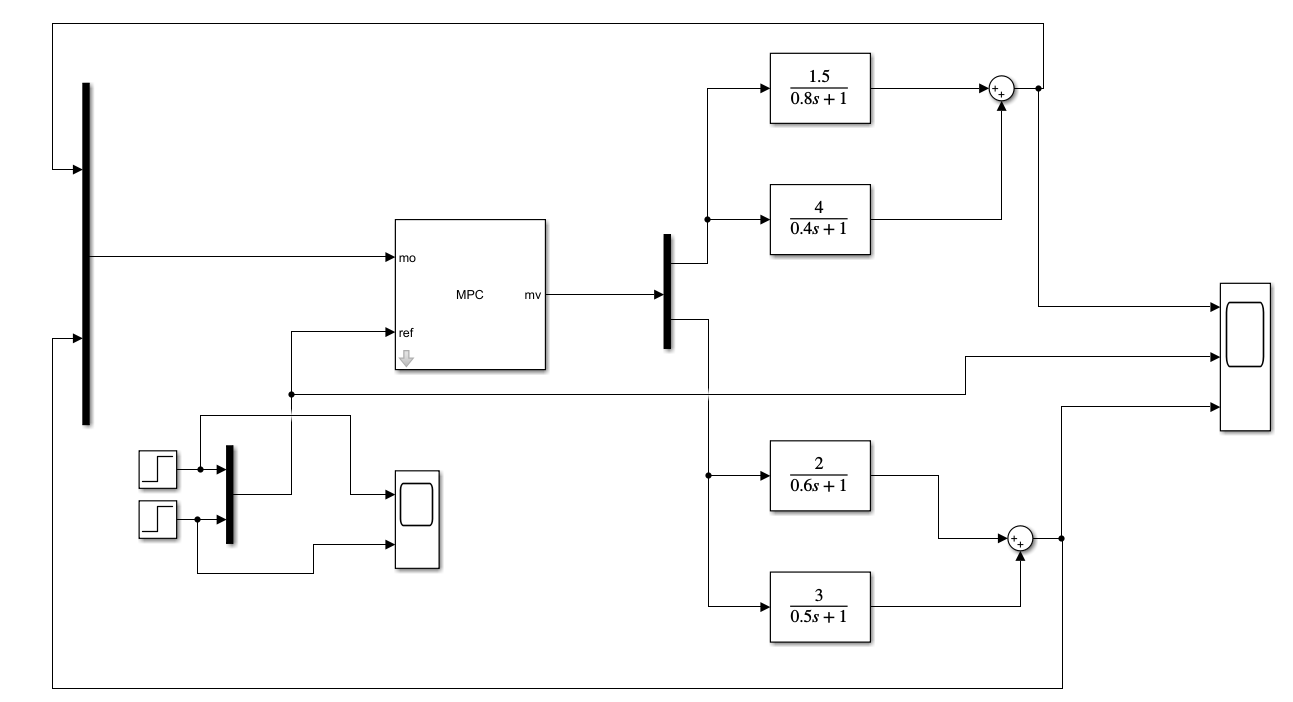
\includegraphics[width=1\linewidth]{../img/Q2_Block_Diagram}
	\caption{بلوک دیاگرام سیستم}
	\label{fig:q2blockdiagram}
\end{figure}

سپس، مقادیر ورودی و رفرنس نیز به وسیله ی بلوک های پله ساخته می شوند.
\begin{figure}[H]
	\centering
	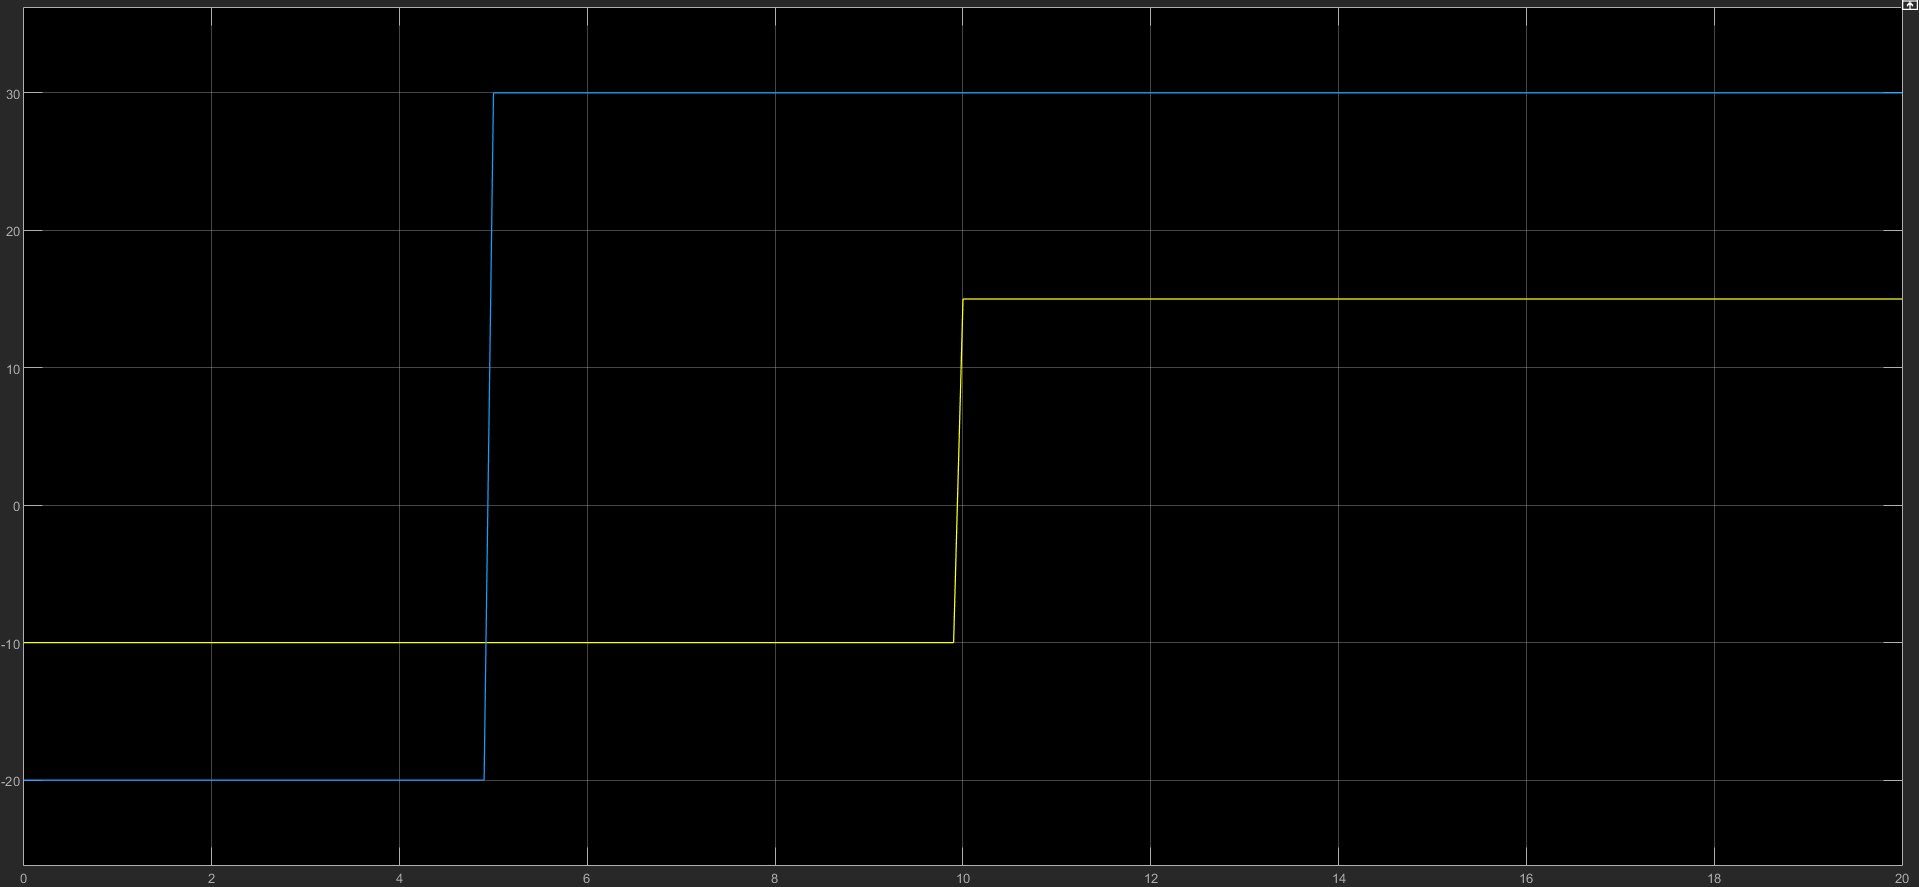
\includegraphics[width=1\linewidth]{../img/Q2_refernece}
	\caption{ورودی های رفرنس}
	\label{fig:q2refernece}
\end{figure}

با سپس، با قرار دادن یک بلوک کنترلر MPC در این سیستم و قرار دادن اسکوپ های مناسب برای بررسی خروجی های سیستم، اقدام به تنظیم پارامترهای کنترلر می کنیم. 
برای این کنترلر، پارامترهای زیر در نظر گرفته شده اند:
\[
\begin{array}{|c|c|}
	\hline
	\textbf{Parameter} & \textbf{Value} \\ 
	\hline
	T_s \, (\text{Sampling Time}) & 0.1 \\ 
	\hline
	\text{Prediction Horizon} & 100 \\ 
	\hline
	\text{Control Horizon} & 20 \\ 
	\hline
\end{array}
\]
همچنین، قید ها و وزن های مطرح شده در سوال نیز برای کنترلر تعریف می شوند.
\begin{figure}[H]
	\centering
	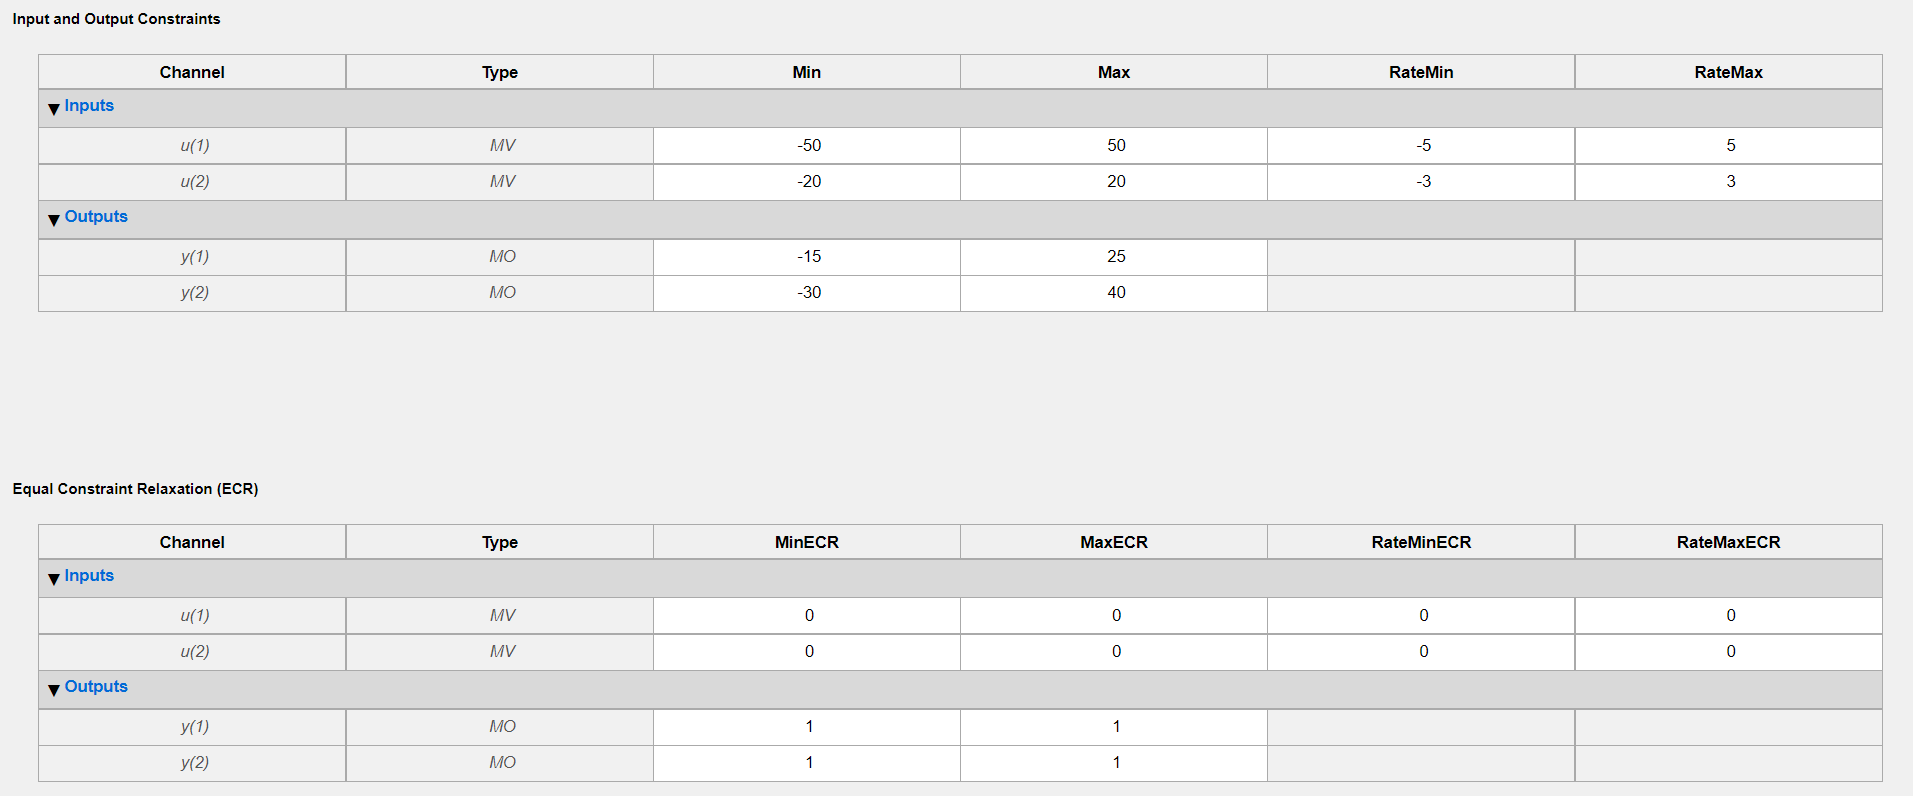
\includegraphics[width=1\linewidth]{../img/Q2_constraints}
	\caption{قیدها}
	\label{fig:q2constraints}
\end{figure}

\begin{figure}[H]
	\centering
	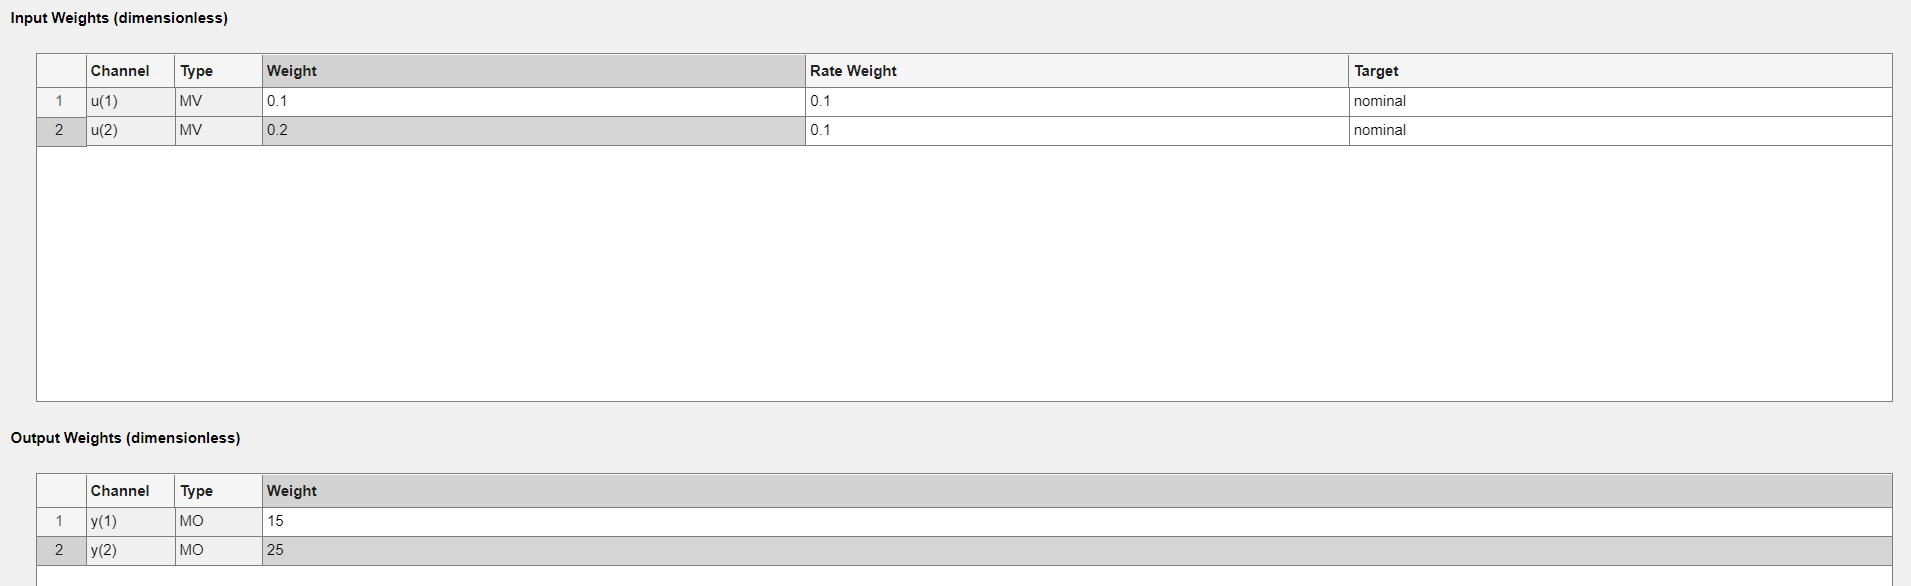
\includegraphics[width=1\linewidth]{../img/Q2_weights}
	\caption{وزن ها}
	\label{fig:q2weights}
\end{figure}

در پایان، با اجرای برنامه مشاهده می شود که کنترلر طراحی شده قادر است با عملکرد مناسبی مقادیر رفرنس را دنبال کنید.
\begin{figure}
	\centering
	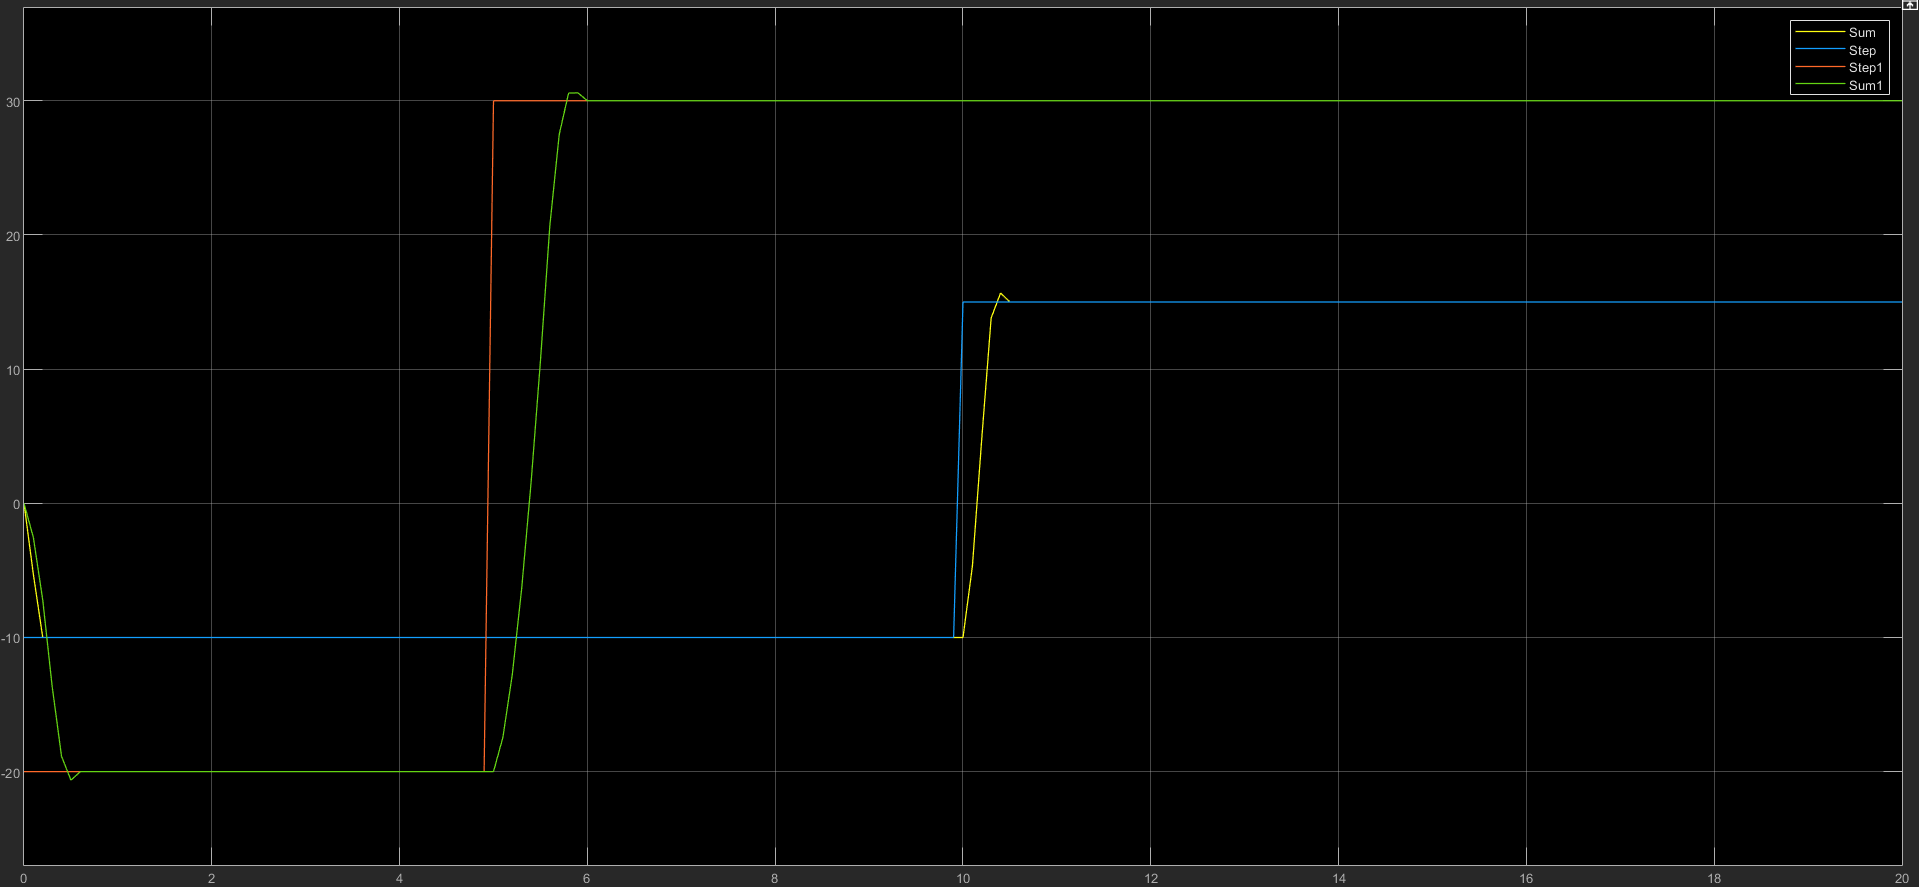
\includegraphics[width=1\linewidth]{../img/Q2_output}
	\caption{پاسخ سیستم}
	\label{fig:q2output}
\end{figure}

\subsection{بخش دوم}
در این بخش، پارامترهای سیستم شامل وزن ها، نرخ نمونه برداری، و افق پیش بین و کنترل را تغییر می دهیم.
\[
\begin{array}{|c|c|}
	\hline
	\textbf{Parameter} & \textbf{Value} \\ 
	\hline
	T_s \, (\text{Sampling Time}) & 0.3 \\ 
	\hline
	\text{Prediction Horizon} & 200 \\ 
	\hline
	\text{Control Horizon} & 40 \\ 
	\hline
\end{array}
\]

 و وزن ها نیز به صورت برابر تغییر داده شده اند:
 \begin{figure}
 	\centering
 	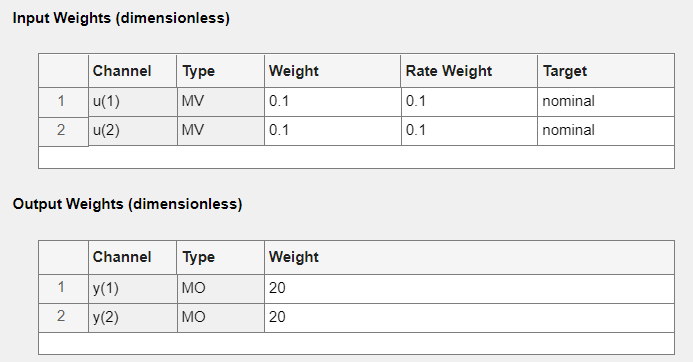
\includegraphics[width=1\linewidth]{../img/Q2_weights_updated}
 	\caption{وزن های تغییر یافته}
 	\label{fig:q2weightsupdated}
 \end{figure}
 
 در این شرایط، مشاهده می کنیم که خروجی های سیستم در مقایسه با حالت اول دارای فراجهش کمتر اما زمان خیزش و نشست بیشتری است.
 \begin{figure}
 	\centering
 	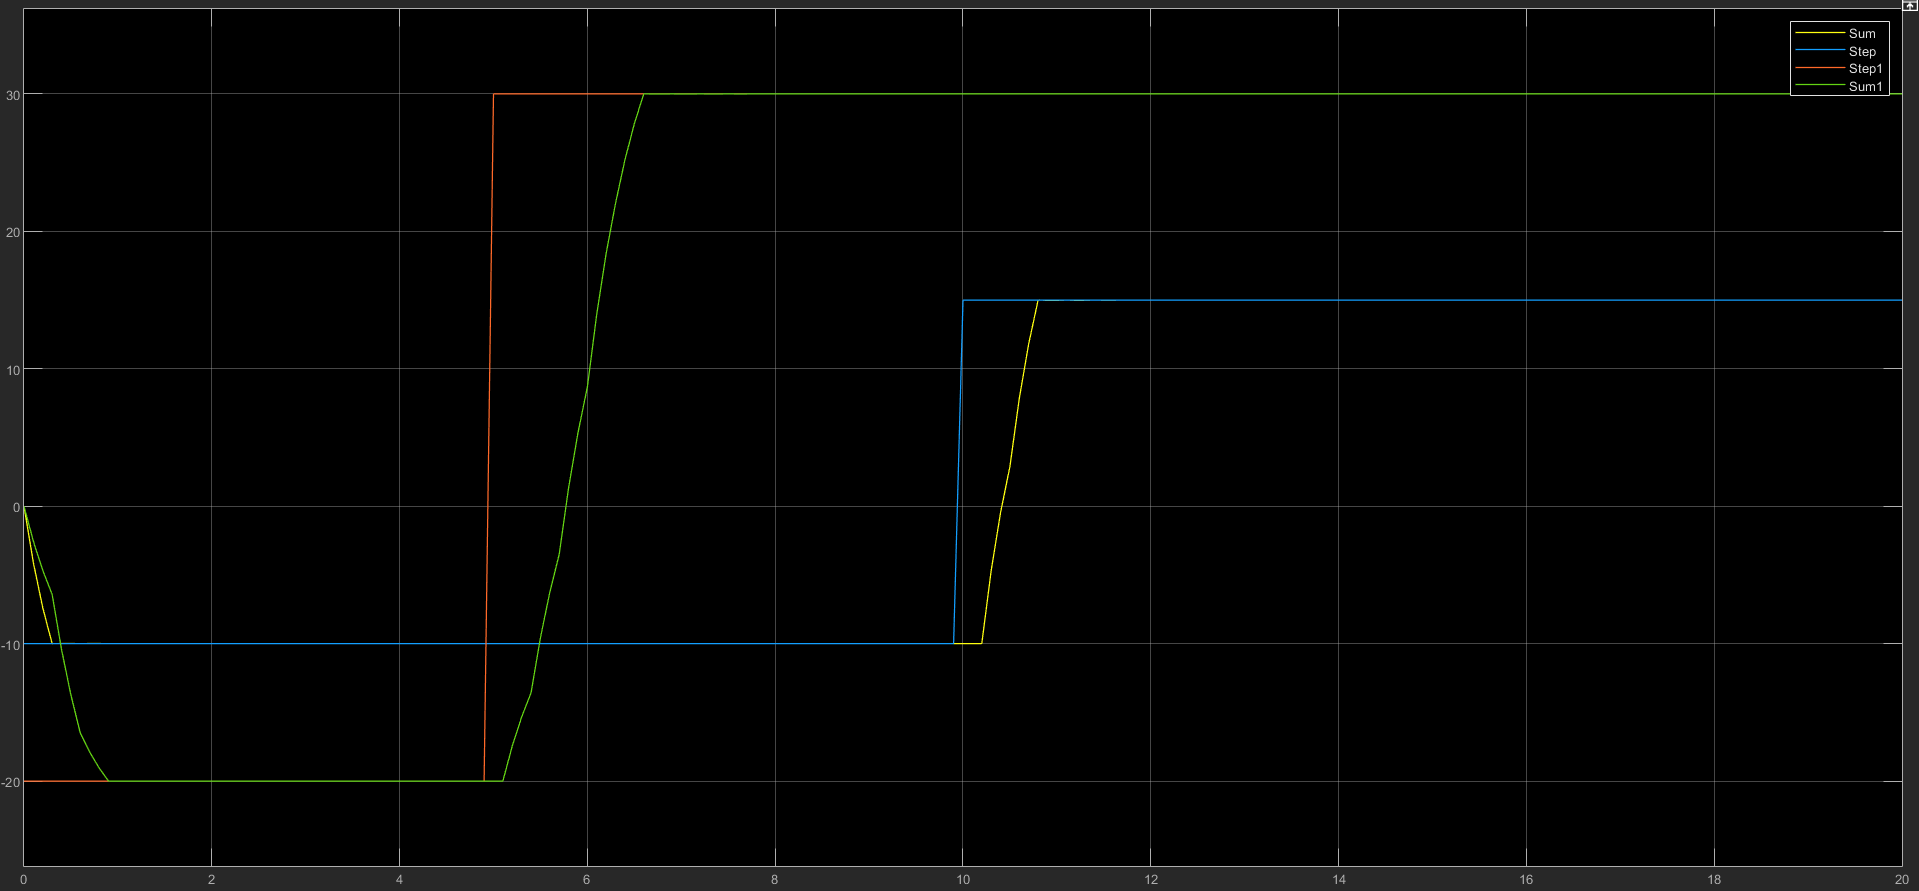
\includegraphics[width=1\linewidth]{../img/Q2_output_updated}
 	\caption{}
 	\label{fig:q2outputupdated}
 \end{figure}
 

\section{پاسخ سوال 3}
\subsection{بخش یکم}
در بخش ابتدایی از این سوال، با در اختیار داشتن ماتریس های حالت سیستم، مدل سیستم را در متلب تعریف کرده و ویژگی های آن را بررسی می کنیم. 
ابتدا قطب ها و صفر های سیستم را مطابق بخش زیر به دست می آوریم:
\[
\text{Poles} = 0, -470.4125, \textcolor{red}{6.7897}, -6.5872
\]

\[
\text{zeros} = -7.1060, 7.1040, 0.0161
\]

مشاهده می شود که این سیستم دارای یک قطب در مبدا و همچنین یک قطب سمت راست است. بنابراین، می توان انتظار داشت که در حالت طبیعی و بدون اعمال کنترلر، سیستم رفتار پایداری نداشته باشد.
این نتیجه را با رسم صفر و قطب های این سیستم نیز می توانیم مشاهده کنیم
\begin{figure}
	\centering
	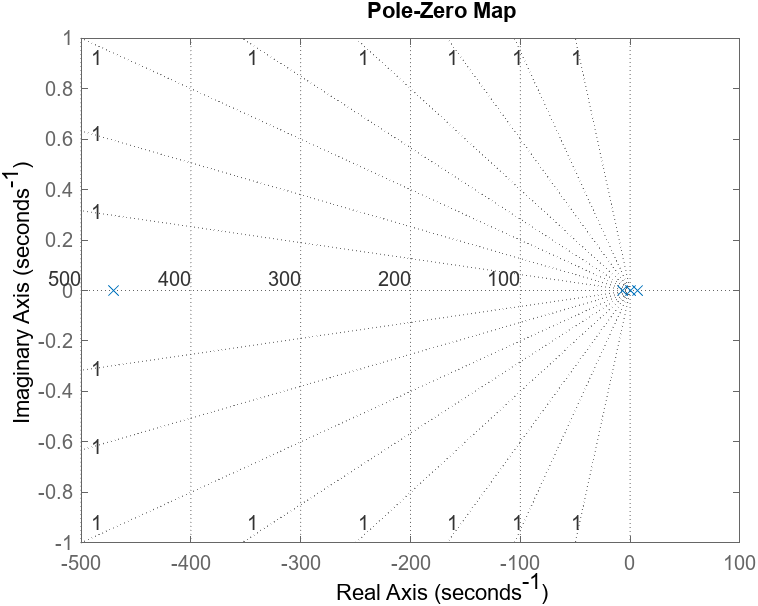
\includegraphics[width=0.7\linewidth]{../img/continues_Poles}
	\caption{}
	\label{fig:continuespoles}
\end{figure}

سپس، برای بررسی رویت پذیری و کنترل پذیری این سیستم، با بررسی رنک ماتریس های زیر می توانیم پاسخ را بیابیم. در صورتی که این ماتریس ها رنک کاملی داشته باشند، آنگاه می توان نتیجه گرفت که کنترل پذیر و یا رویت پذیر هستند. 

با بررسی سیستم مورد استفاده در این قسمت، می بینیم که این ماتریس هم \textbf{رویت پذیر} و هم \textbf{کنترل پذیر} است

پس از به دست آوردن مدل حالت سیستم در بخش قبل، در اینجا آن را به یک مدل گسسته تبدیل می کنیم. برای این کار، با استفاده از دستور
 c2d
  سیستم را گسسته می کنیم. در گام بعد، ماتریس های حالت این سیستم گسسته از مدل برای استفاده های بعدی استخراج می شود. حال، مجددا صفر و قطب های این سیستم را به دست آورده و آنها را رسم می کنیم.
	
\begin{figure}[H]
	\centering
	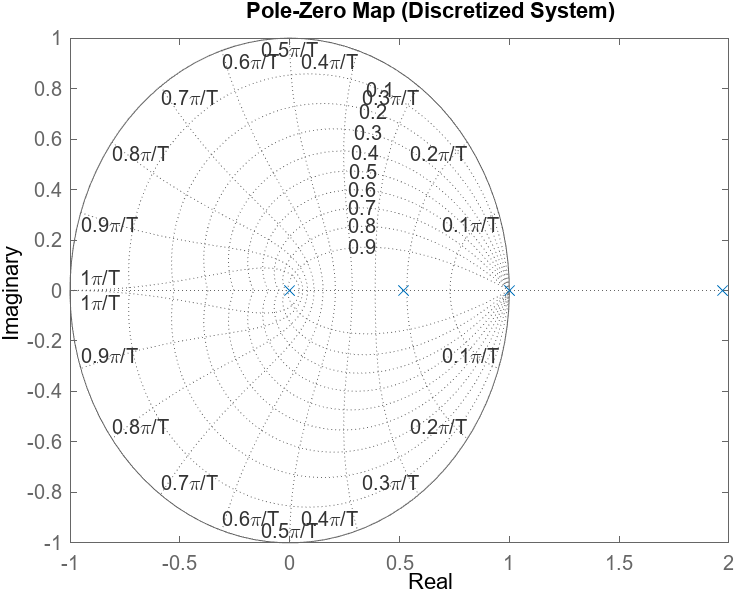
\includegraphics[width=0.7\linewidth]{../img/discrete_Poles}
	\caption{}
	\label{fig:discretepoles}
\end{figure}

در نهایت، پاسخ پله ی این سیستم را رسم می کنیم. اما انتظار داریم که پاسخی ناپایدار به دست بیاید.
\begin{figure}[H]
	\centering
	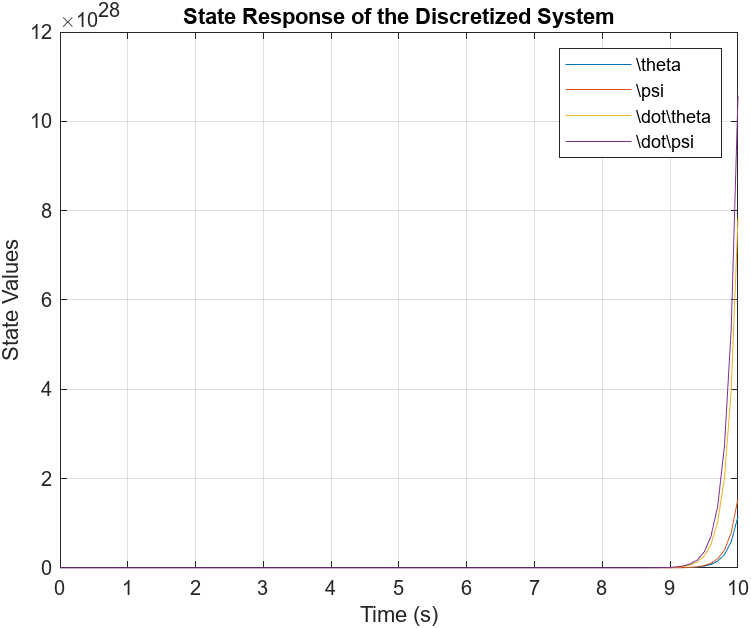
\includegraphics[width=0.9\linewidth]{../img/discrete_response}
	\caption{}
	\label{fig:discreteresponse}
\end{figure}


\subsection{بخش دوم}
	در این بخش، ابتدا سیستم در محیط سیمولینک تعریف شده و برای گام اول، پاسخ حالت صفر آن را نمایش می دهیم. همچنین شرایط اولیه مورد استفاده نیز در حالت اولیه برای بلوک معادلات حالت سیستم لحاظ می شود.
	\[
	x_0 = [0, 0.1, 0, 0]
	\]
	
\begin{figure}[H]
	\centering
	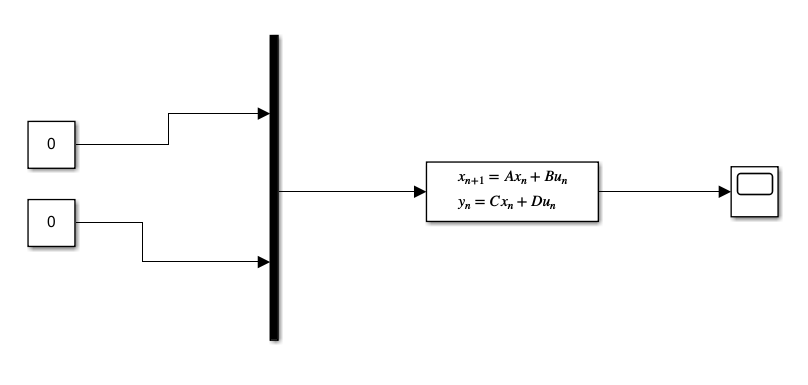
\includegraphics[width=0.7\linewidth]{../img/system_Zero_Responce_Simulink}
	\caption{}
	\label{fig:systemzeroresponcesimulink}
\end{figure}

با اجرای برنامه و مشاهده ی نتیجه ی شبیه سازی، مجددا مشاهده می کنیم که پاسخ سیستم ناپایدار بوده و به بی نهایت میل می کند.
	
 
\begin{figure}[H]
	\centering
	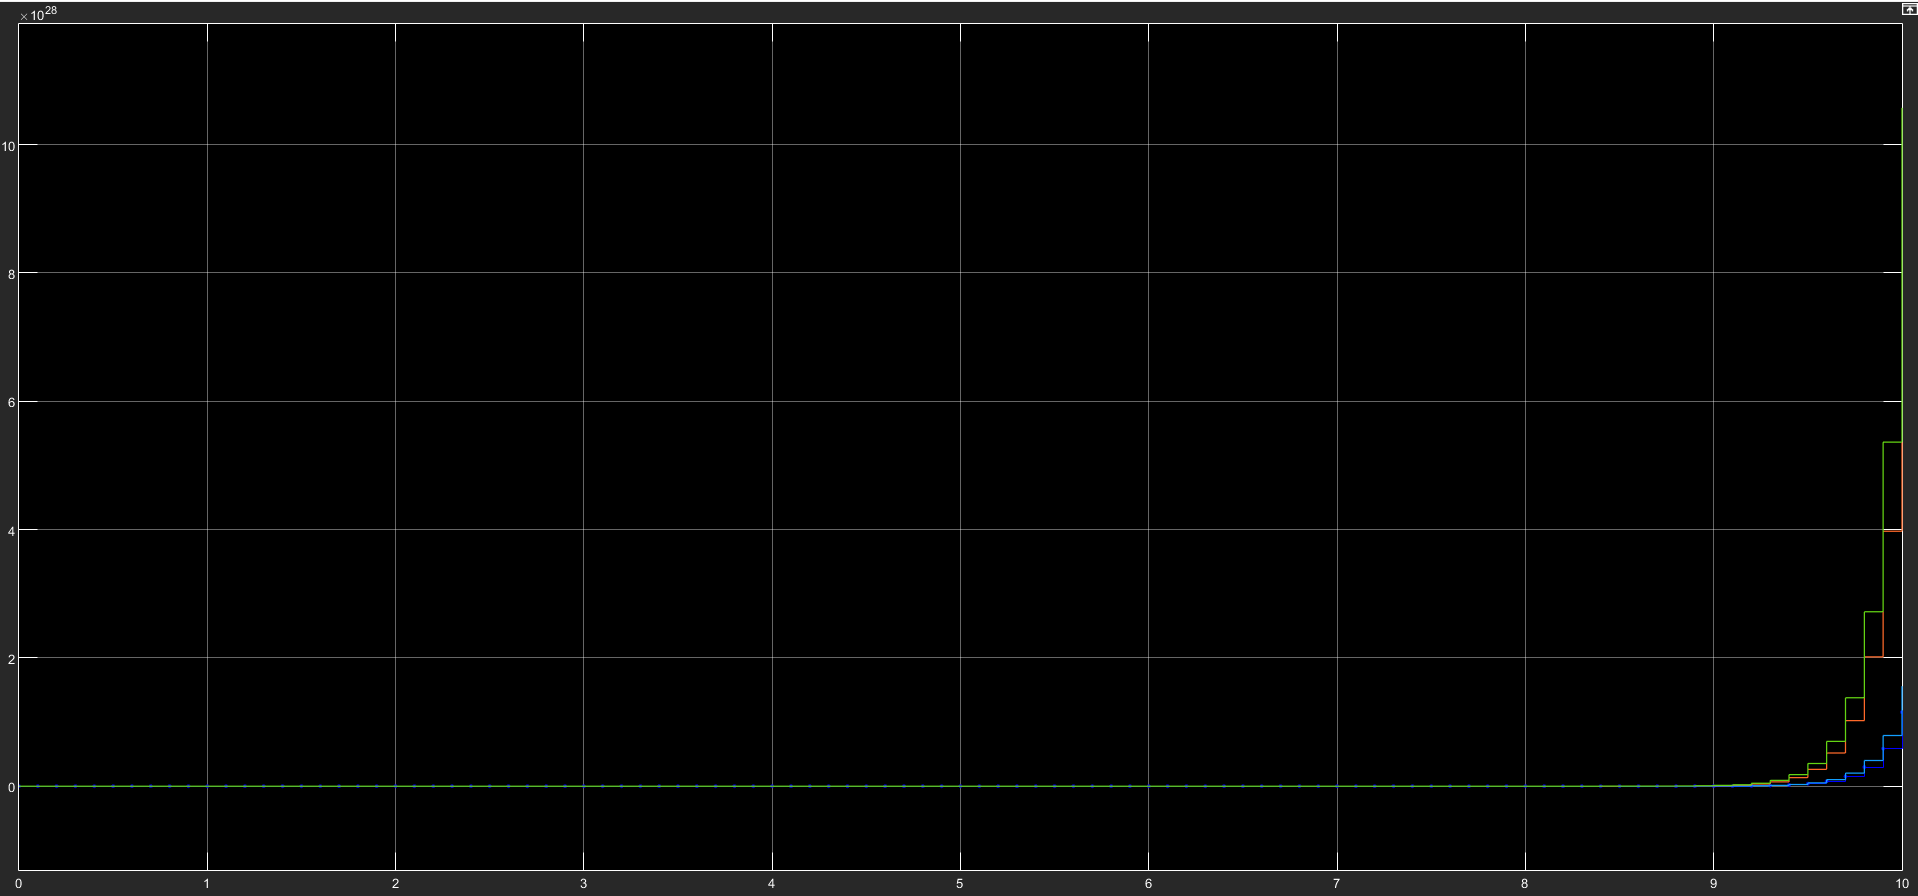
\includegraphics[width=1\linewidth]{../img/Q2_Zero_Response}
	\caption{}
	\label{fig:q3zeroresponse}
\end{figure}
 
 در این مثال و بخش پیشین، بازه زمانی نمونه برداری بر روی 0.1 ثانیه تنظیم شده است.
 
 \subsection{بخش سوم}
 در بخش سوم، بر روی سیستم طراحی شده، دو کنترلر MPC و LQR پیاده سازی می شود. همچنین، اغتشاشی به اندازه ی 0.05 در بازه زمانی بین ثانیه های 4 و 5 به سیستم اعمال می شود. 
 
 \begin{figure}
 	\centering
 	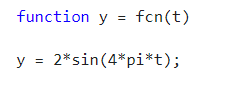
\includegraphics[width=1\linewidth]{../img/Q3_Disturbance}
 	\caption{}
 	\label{fig:q3disturbance}
 \end{figure}
 
 \subsubsection{MPC}
 برای ساخت اغتشاش، از دو بلوک پله با علامت های متفاوت استفاده شده است. بلوک دیاگرام این سیستم در بخش زیر نمایش داده شده است.
 
\begin{figure}[H]
	\centering
	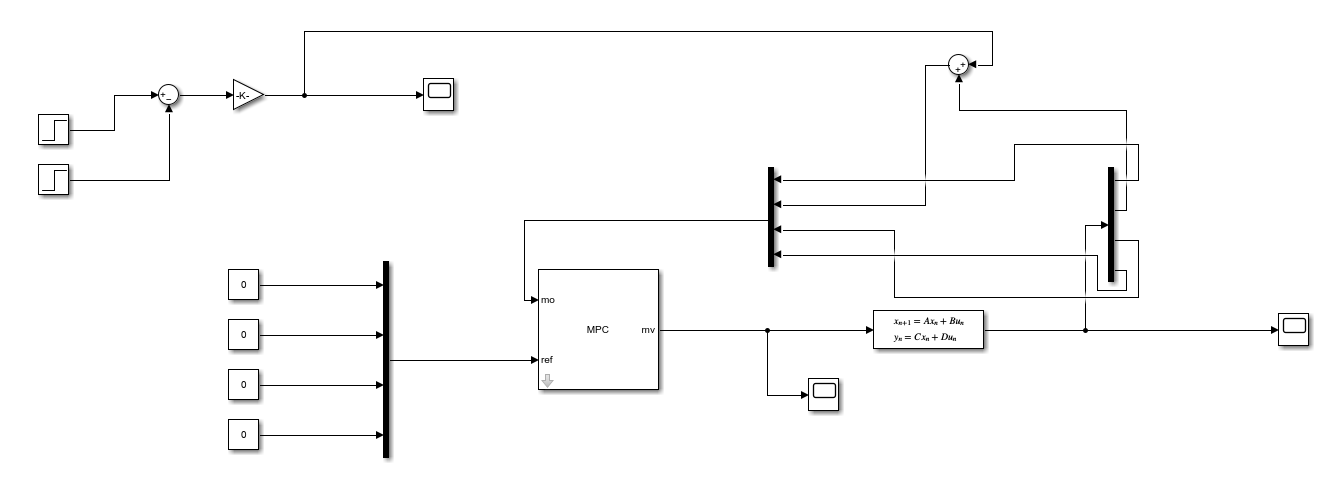
\includegraphics[width=1\linewidth]{../img/Q3_MPC_Block}
	\caption{}
	\label{fig:q3mpcblock}
\end{figure}
 
 تنظیم پارامتر های بلوک کنترلر MPC با مقادیر زیر تنظیم شده است:
 
 \[
 \begin{array}{|c|c|}
 	\hline
 	\textbf{Parameter} & \textbf{Value} \\ 
 	\hline
 	T_s \, (\text{Sampling Time}) & 0.1 \\ 
 	\hline
 	\text{Prediction Horizon} & 20 \\ 
 	\hline
 	\text{Control Horizon} & 10 \\ 
 	\hline
 \end{array}
 \]
 
 با اجرای این برنامه، می توانیم پاسخ های خروجی را به صورت زیر مشاهده کنیم:
 
 
 
\begin{figure}[H]
	\centering
	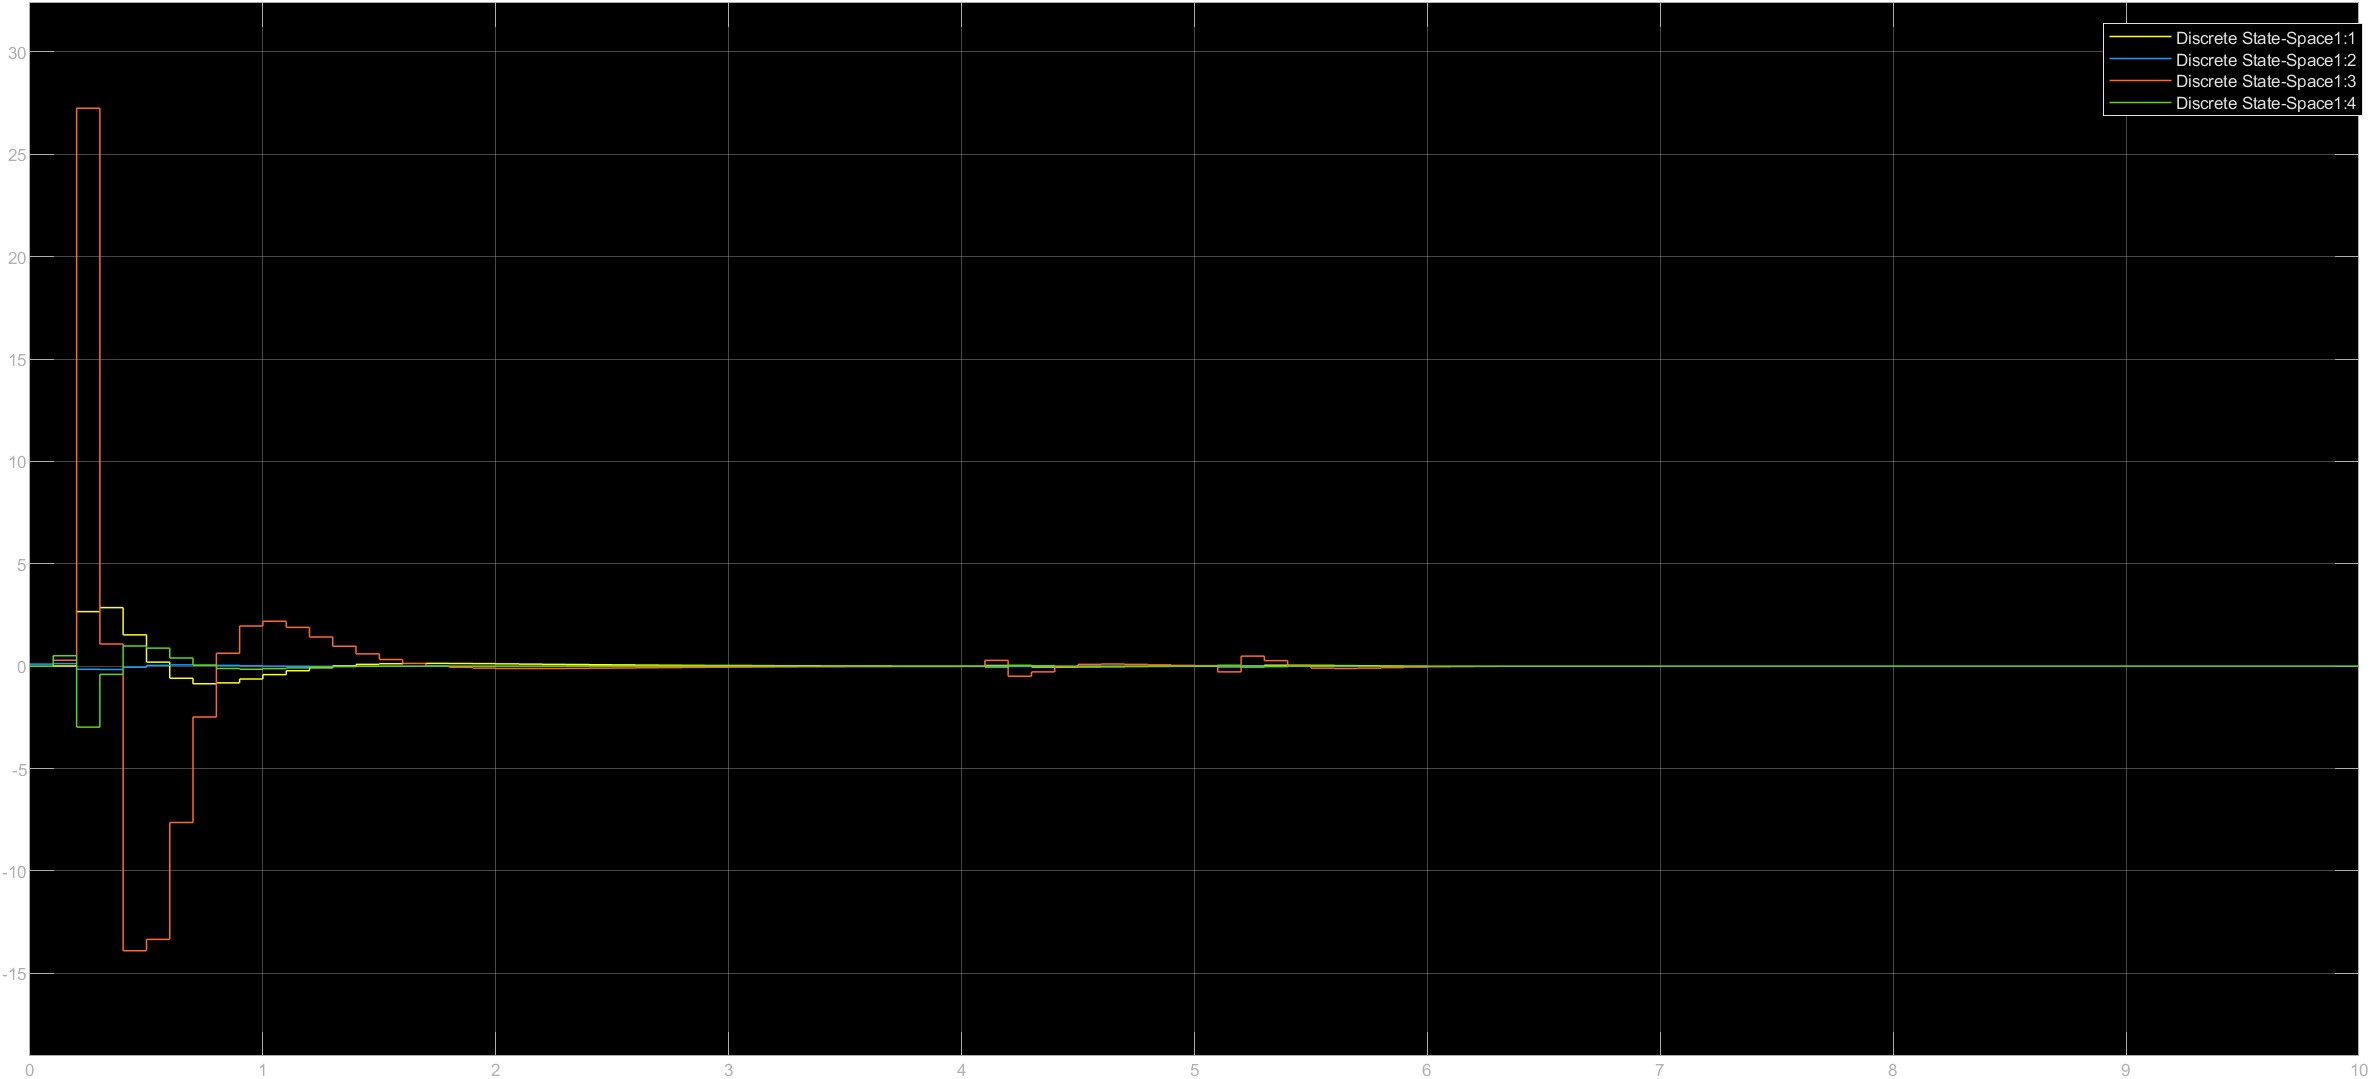
\includegraphics[width=1\linewidth]{../img/Q3_MPC_Output}
	\caption{پاسخ کنترلر MPC}
	\label{fig:q3mpcoutput}
\end{figure}
 
\begin{figure}[H]
	\centering
	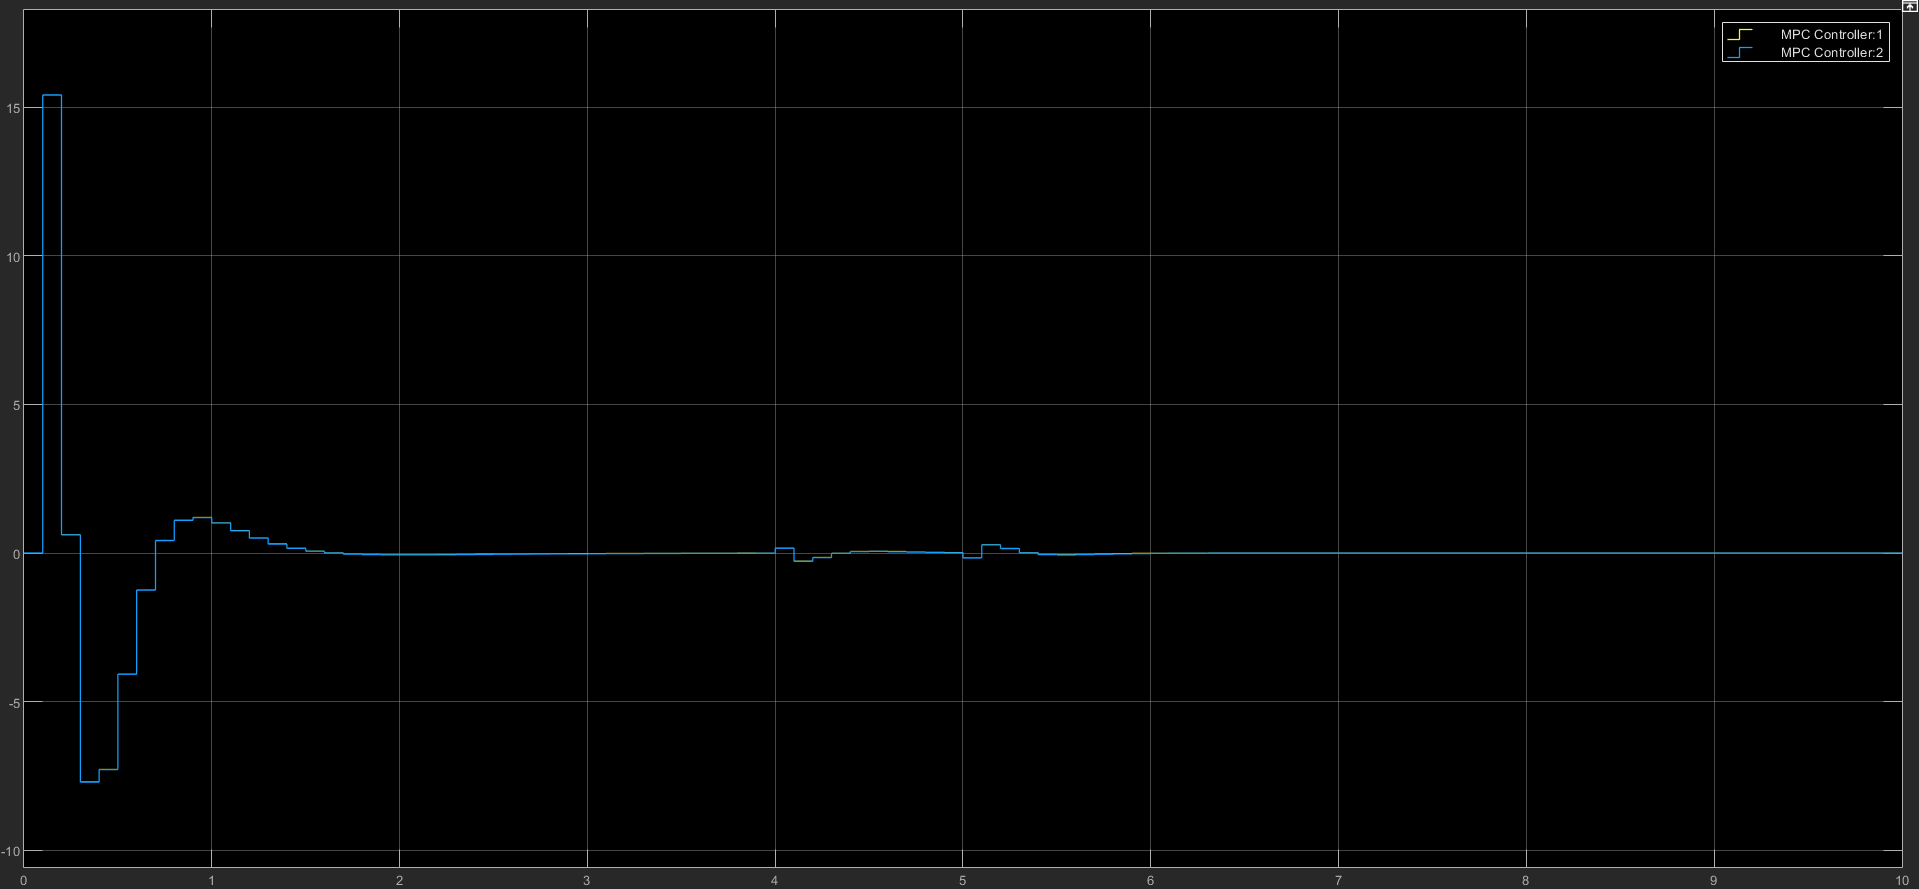
\includegraphics[width=1\linewidth]{../img/Q3_MPC_control_effort}
	\caption{تلاش کنترلی MPC}
	\label{fig:q3mpccontroleffort}
\end{figure}
 
 
 \begin{figure}[H]
 	\centering
 	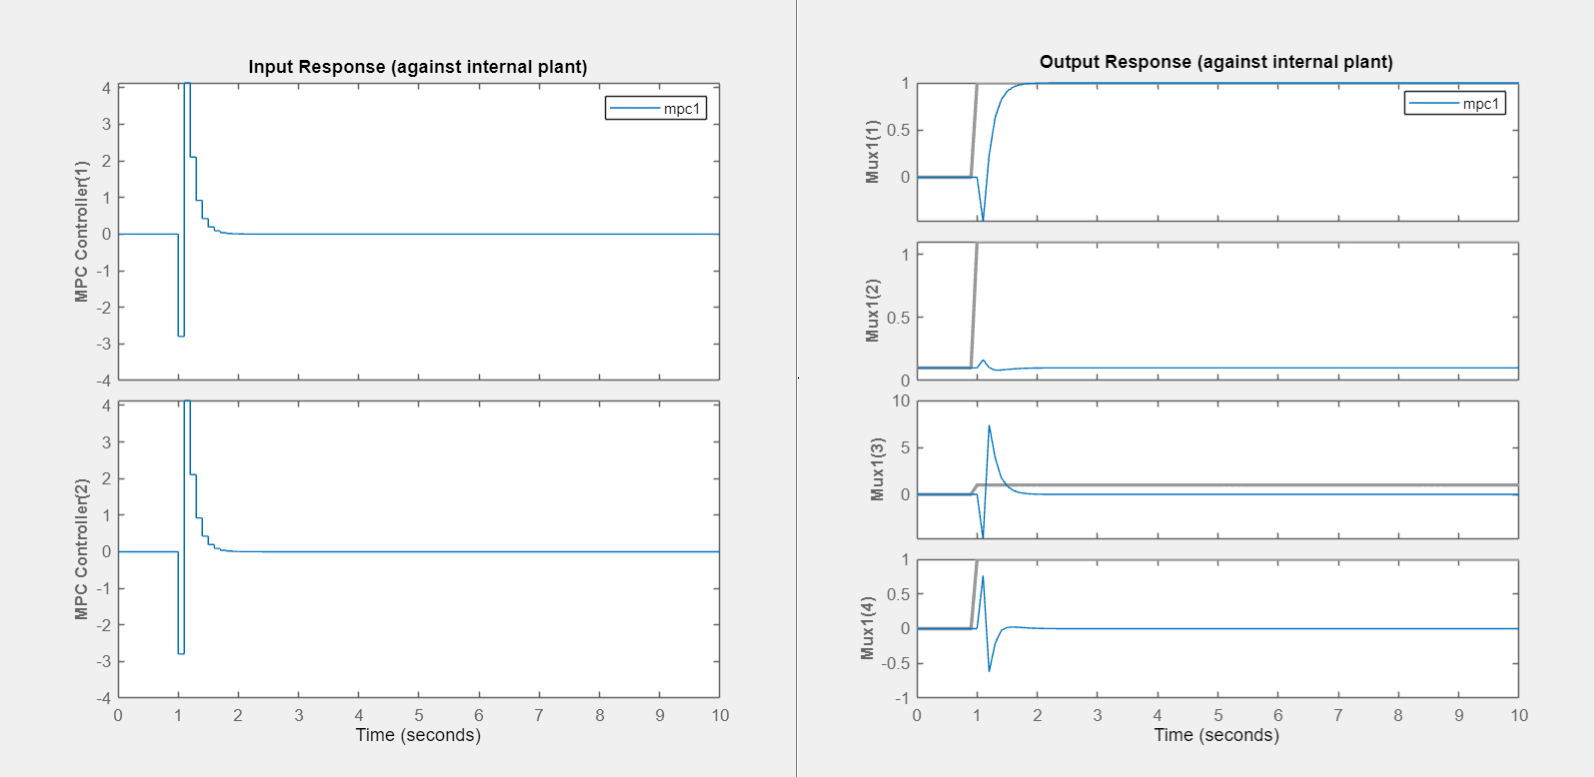
\includegraphics[width=1\linewidth]{../img/Q3_MPC_Setting}
 	\caption{تلاش کنترلی و پاسخ سیستم به ازای هر حالت}
 	\label{fig:q3mpcsetting}
 \end{figure}
 
 چنان که مشاهده می شود، کنترلر MPC مورد استفاده توانسته خروجی های اول و سوم را با میزان خطای قابل قبولی کنترل کند. اما این سیستم برای کنترلر حالت های دوم و چهارم عملکرد مناسبی ندارد و ان چنان که در پاسخ سیستم دیده می شود، در صورت اعمال اغتشاش به خروجی دوم، فراجهش زیادی در پاسخ دریافت خواهیم کرد.
 
 \subsubsection{LQR}
 پ
 برای طراحی و پیاده سازی کنترلر LQR، لازم است یک ماتریس بهره در فیدبک حالت ضرب شود. پیش از پیاده سازی این کنترلر در محیط سیمولینک، با استفاده از مدل سیستم گسسته، پارامتر های مورد نیاز برای محاسبه ی مقادیر این بهره به دست می آید. برای این منظور، با استفاده از دو ماتریس A و B و همچنین تعریف دو ماتریس جدید R و Q، می توانیم بهره را به دست بیاوریم. 
 با استفاده از دستور dlqr، پارامترهای LQR به صورت زیر به دست می آید.
 
\[
k_{LQR} = 
\begin{bmatrix}
	-0.7434 & -60.6744 & -1.0184 & -8.0624 \\
	-0.7434 & -60.6744 & -1.0184 & -8.0624
\end{bmatrix}
\]

\[
s_{LQR} = 
1.0 \times 10^{5} \cdot
\begin{bmatrix}
	0.0067 & 0.0793 & 0.0014 & 0.0111 \\
	0.0793 & 2.1697 & 0.0381 & 0.3005 \\
	0.0014 & 0.0381 & 0.0008 & 0.0053 \\
	0.0111 & 0.3005 & 0.0053 & 0.0418
\end{bmatrix}
\]

\[
p_{LQR} = 
\begin{bmatrix}
	0.7348 + 0.0000i \\
	0.4950 + 0.0215i \\
	0.4950 - 0.0215i \\
	-0.0000 + 0.0000i
\end{bmatrix}
\]

 
 با قرار دادن مقدار به دست آمده برای K در بلوک کنترلی طراحی شده برای این سیستم که در قسمت پایین نمایش داده شده است، می توانیم برنامه را اجرا کنیم:
 
 \begin{figure}[H]
 	\centering
 	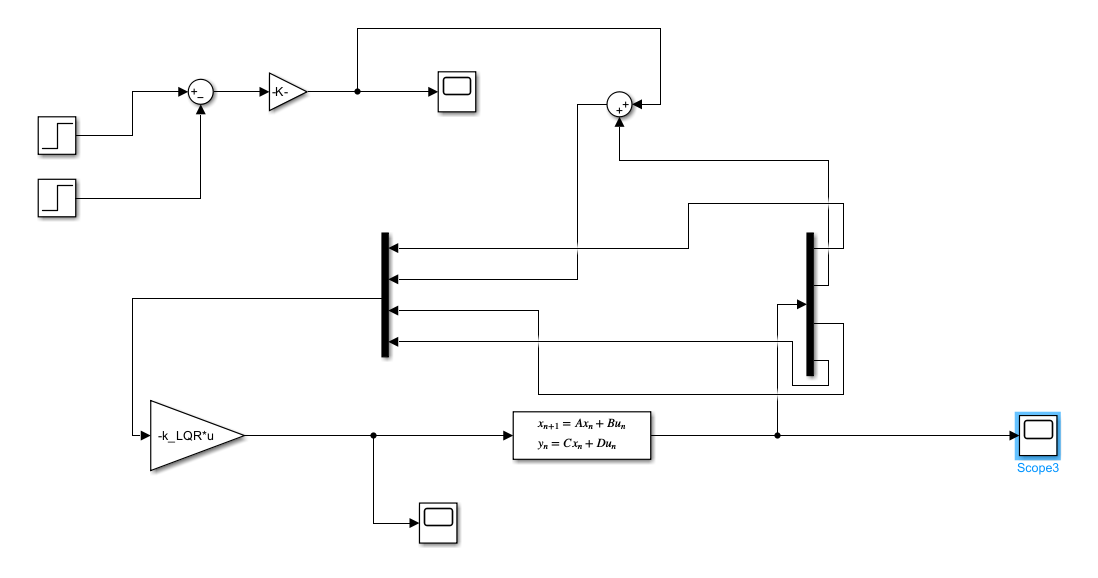
\includegraphics[width=1\linewidth]{../img/Q3_LQR_Block}
 	\caption{بلوک دیاگرام کنترلر LQR}
 	\label{fig:q3lqrblock}
 \end{figure}
 
 \begin{figure}[H]
 	\centering
 	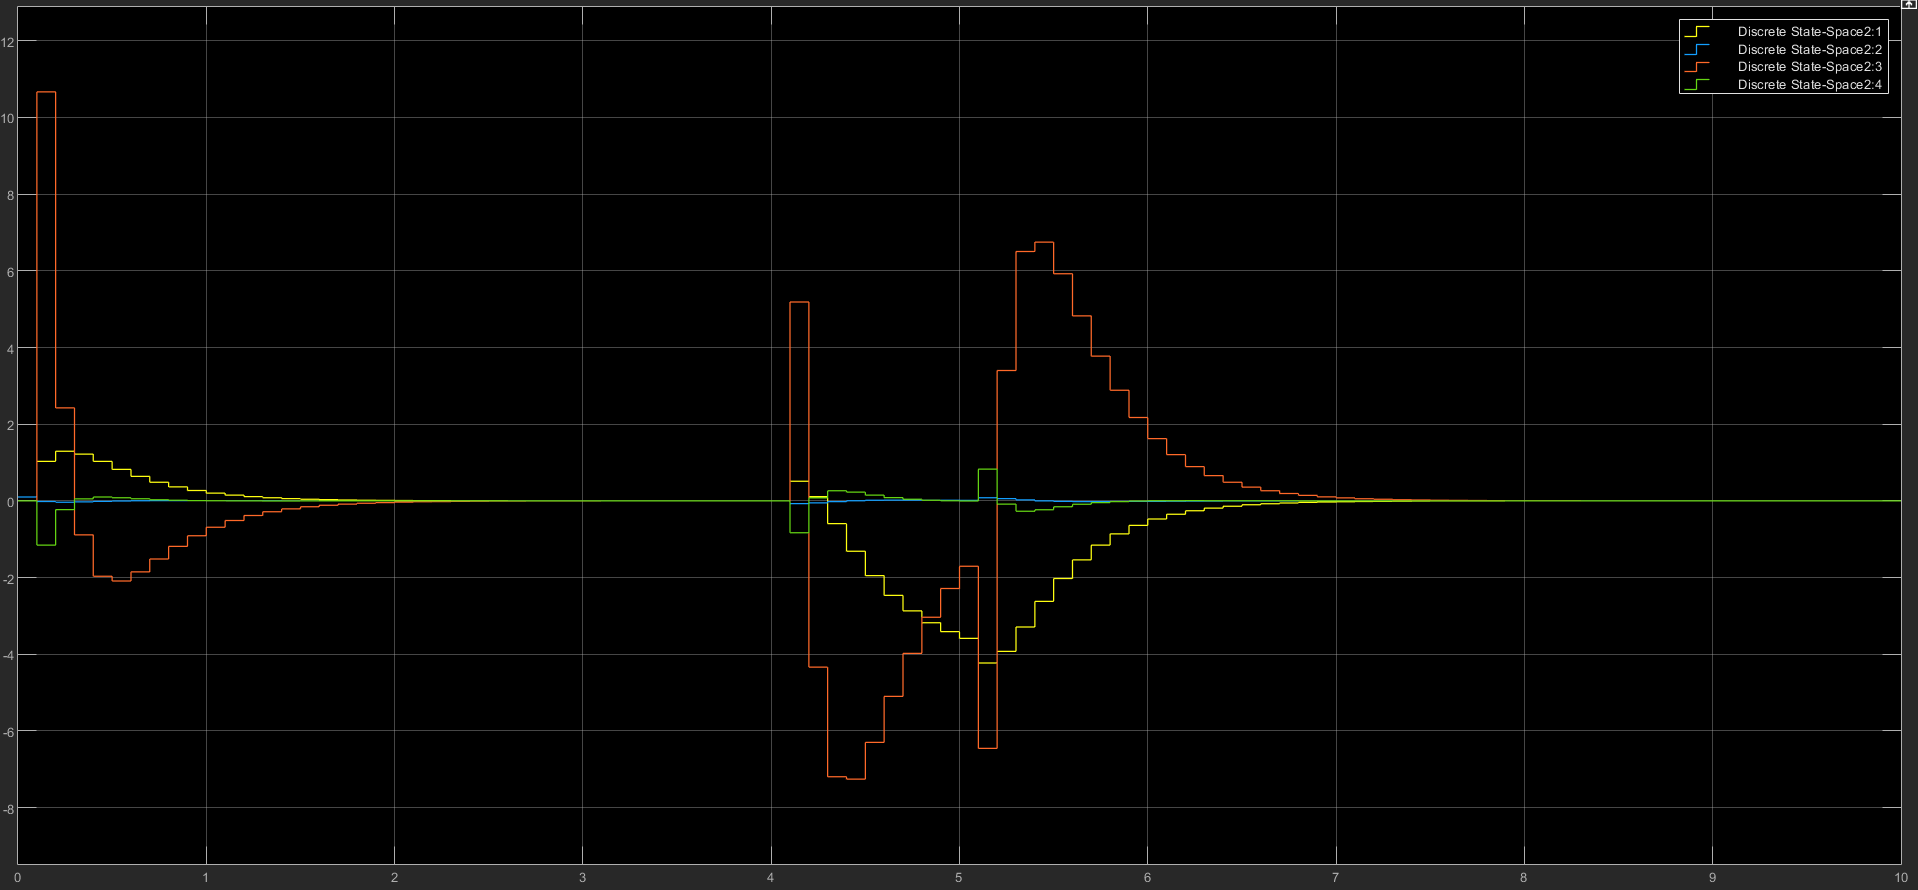
\includegraphics[width=1\linewidth]{../img/Q3_LQR_Output}
 	\caption{پاسخ کنترلر LQR}
 	\label{fig:q3lqroutput}
 \end{figure}
 
 \begin{figure}[H]
 	\centering
 	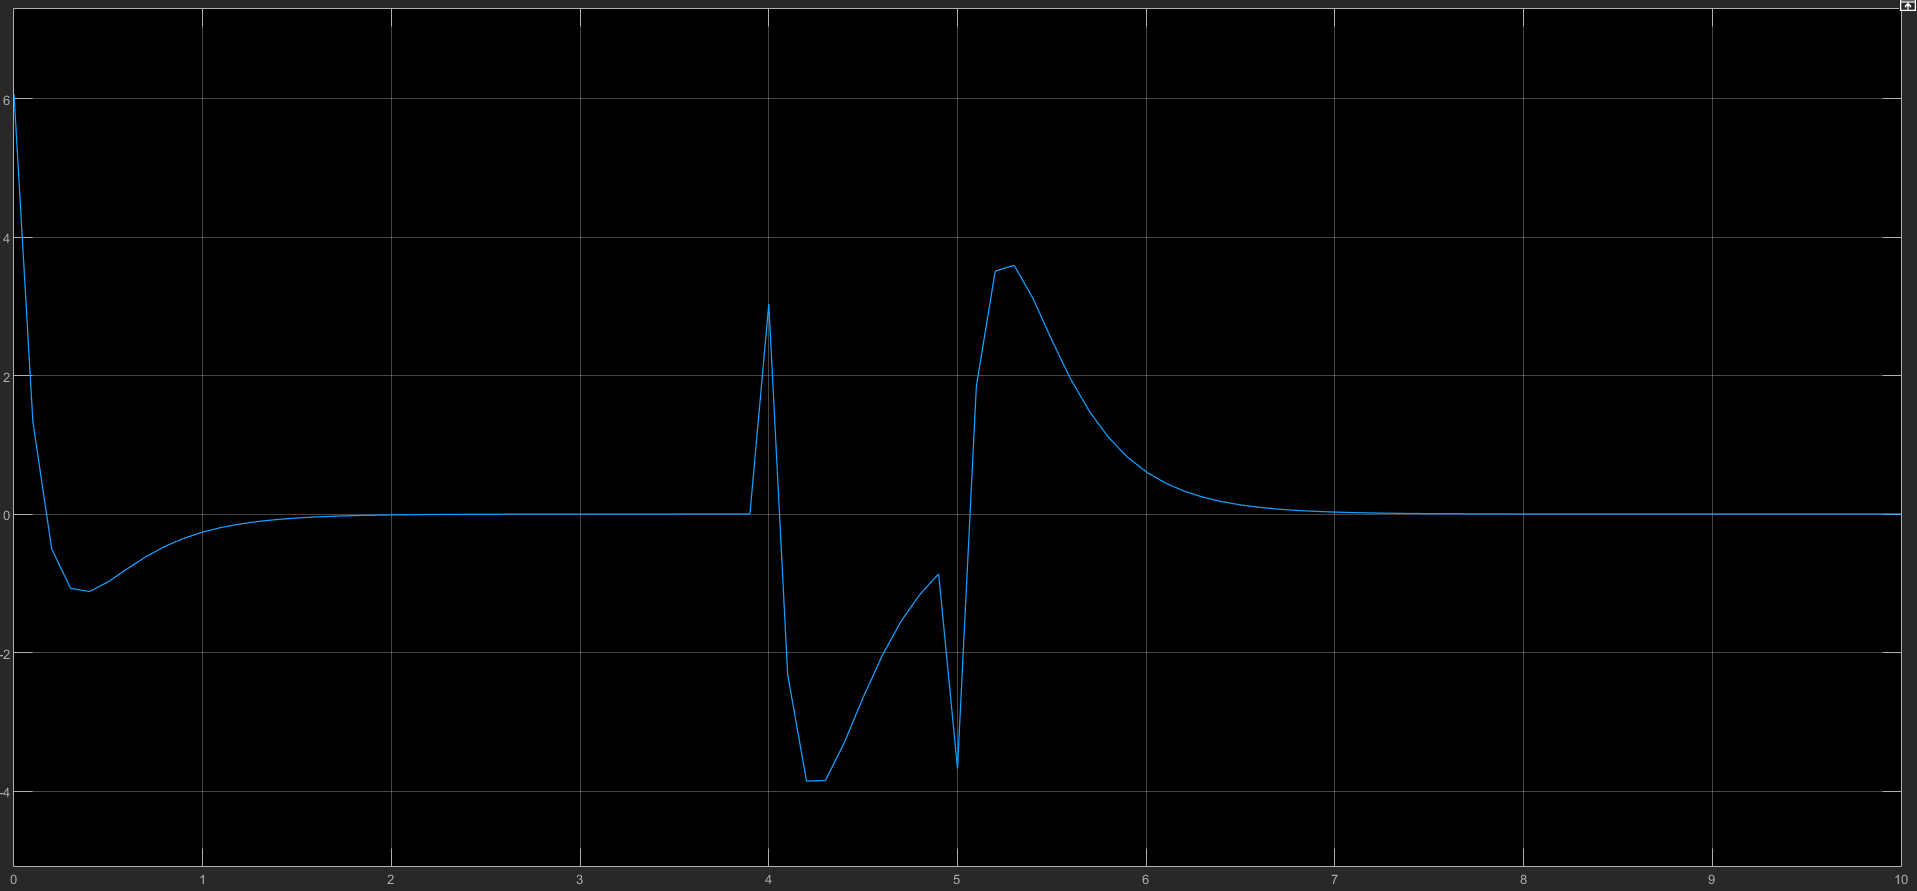
\includegraphics[width=1\linewidth]{../img/Q3_LQR_control_effort}
 	\caption{تلاش کنترلی LQR}
 	\label{fig:q3lqrcontroleffort}
 \end{figure}
 
 مشاهده می شود که این کنترلر نیز می تواند مانند کنترل MPC، خروجی را کنترل کند. با این حال، عملکرد کنترلر در کنترل حالت دوم نتایج قابل قبولی ندارد.
 
\subsection{بخش چهارم}

در این بخش، با لحاظ کردن محدودیت بر روی خروجی اول سیستم در دو حالت سخت و نرم، رفتار سیستم را بررسی می کنیم.
محدودیت این قسمت به صورت زیر تعریف می شود.
\[
-0.3 \leq \theta \leq 1.5
\]

\subsubsection{سخت}

با تنظیم محدودیت ها و اجرای برنامه در حالت سخت خواهیم داشت:
\begin{figure}[H]
	\centering
	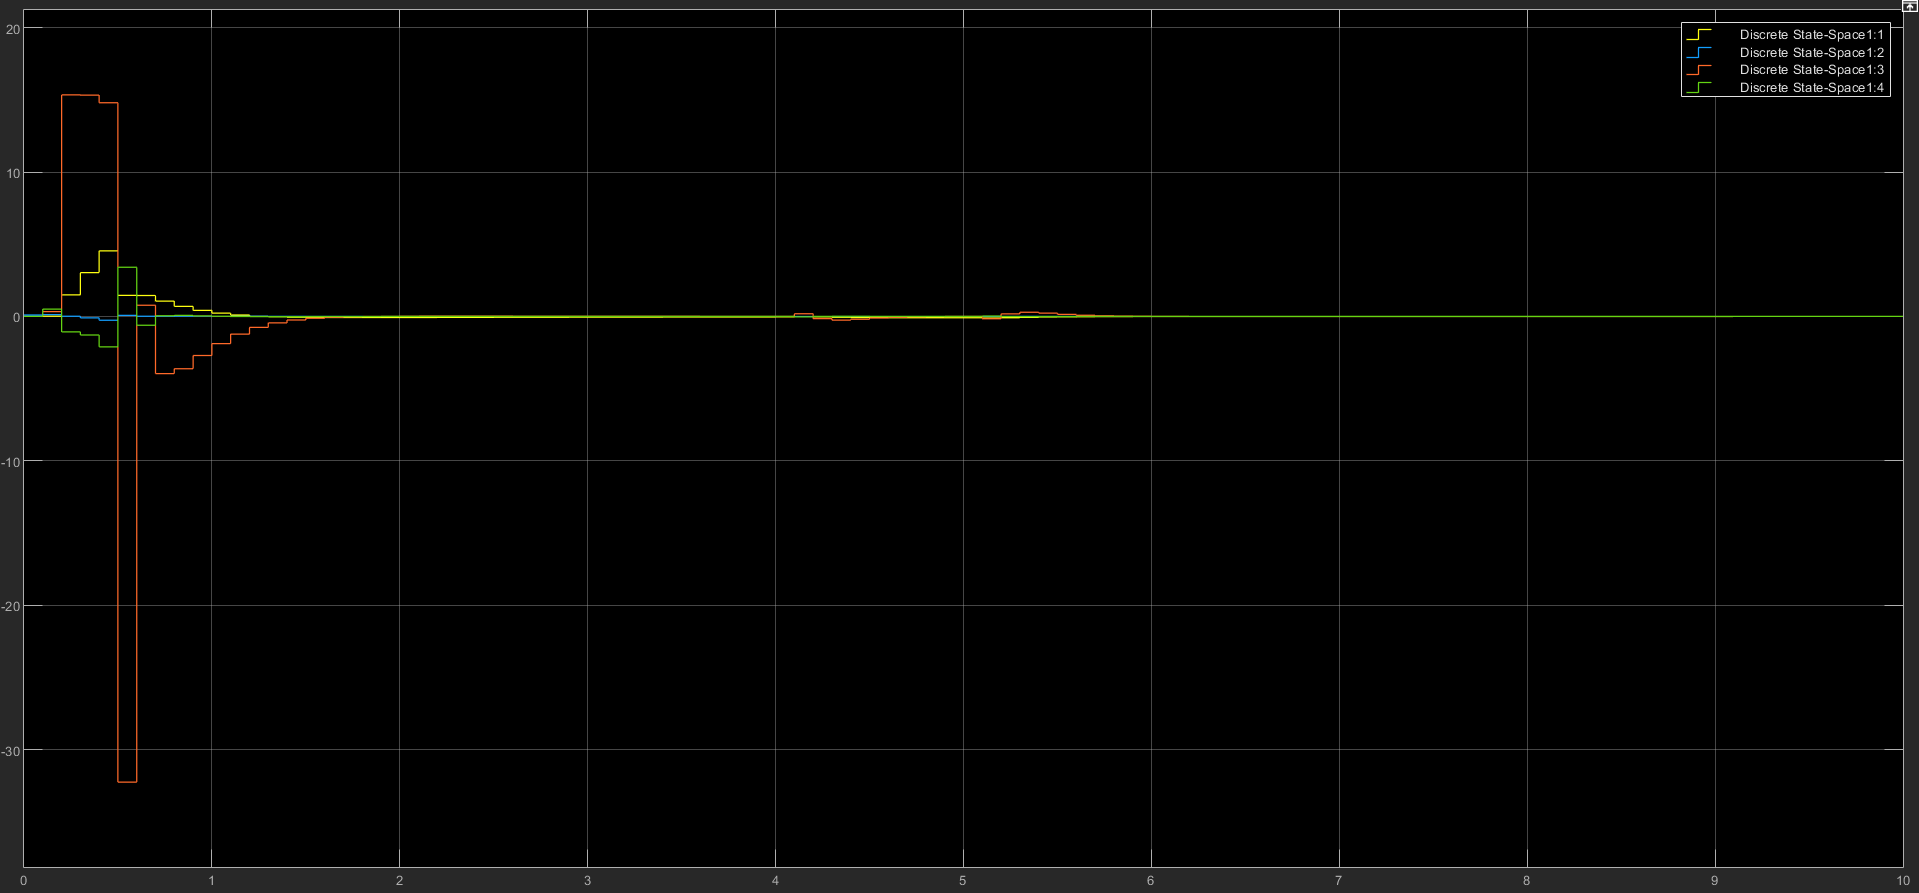
\includegraphics[width=1\linewidth]{../img/Q4_Hard_Output}
	\caption{پاسخ کنترلر MPC محدود با قید های سخت}
	\label{fig:q4hardoutput}
\end{figure}

\begin{figure}[H]
	\centering
	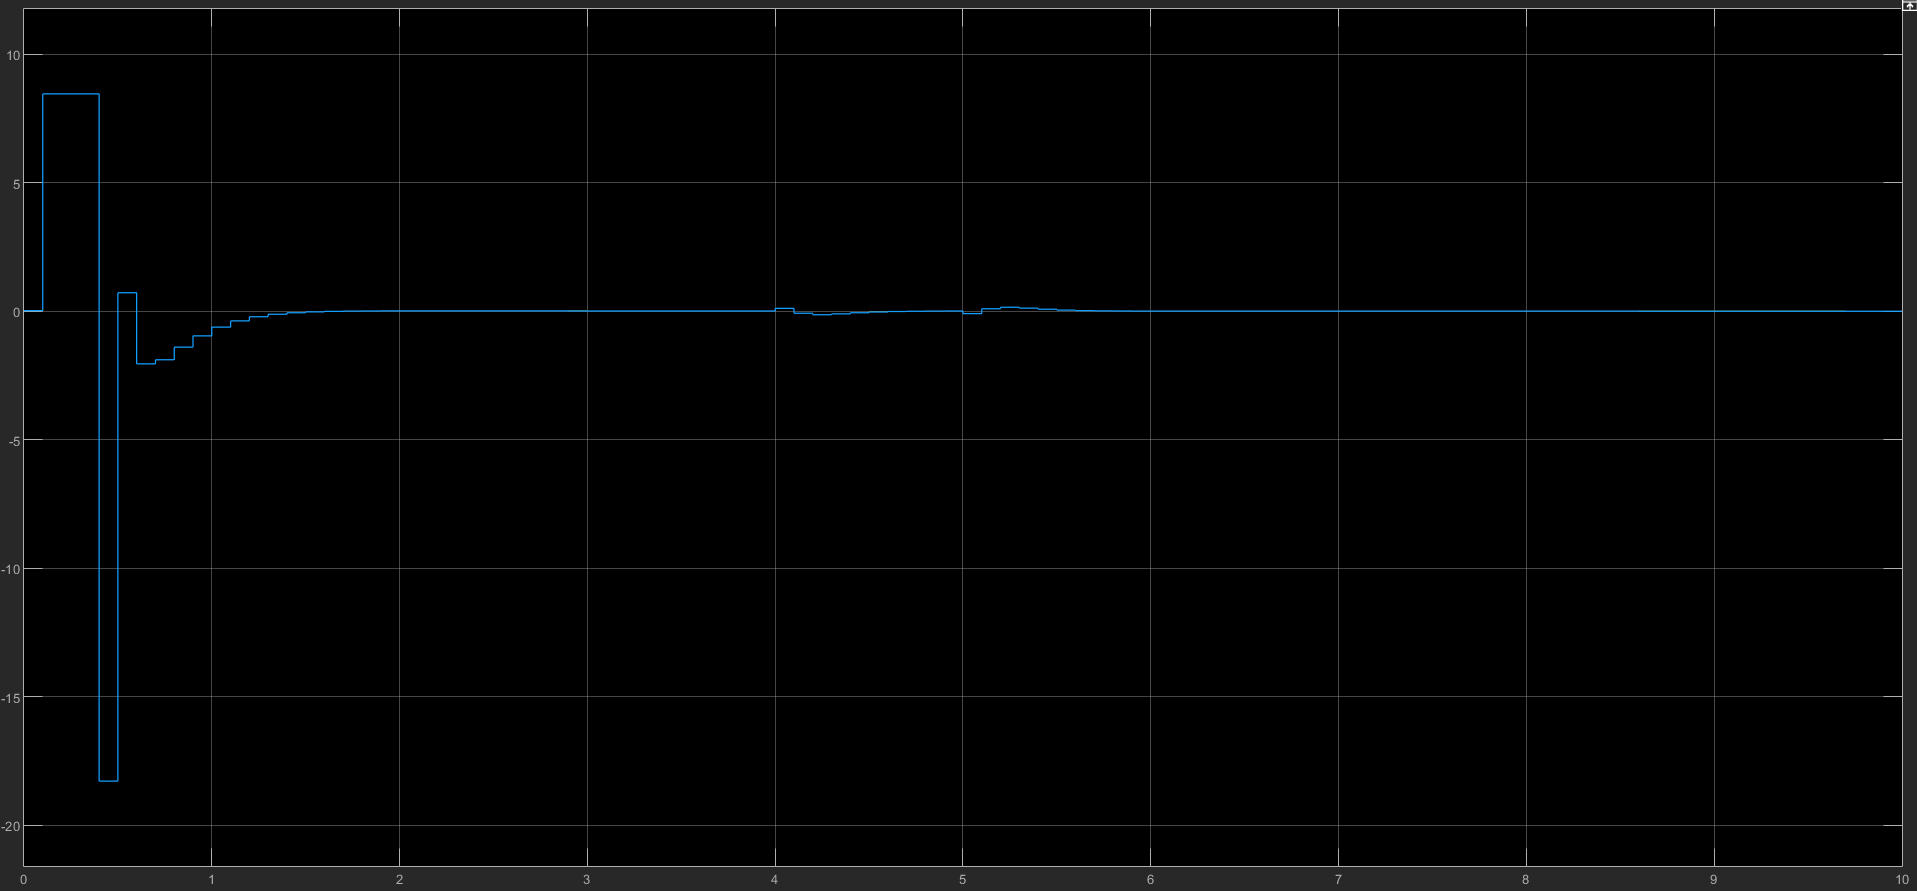
\includegraphics[width=1\linewidth]{../img/Q4_Hard_control_effort}
	\caption{تلاش کنترلی کنترلر MPC با قید های سخت}
	\label{fig:q4hardcontroleffort}
\end{figure}

\subsubsection{نرم}
با تنظیم محدودیت ها و اجرای برنامه در حالت نرم خواهیم داشت:
\begin{figure}[H]
	\centering
	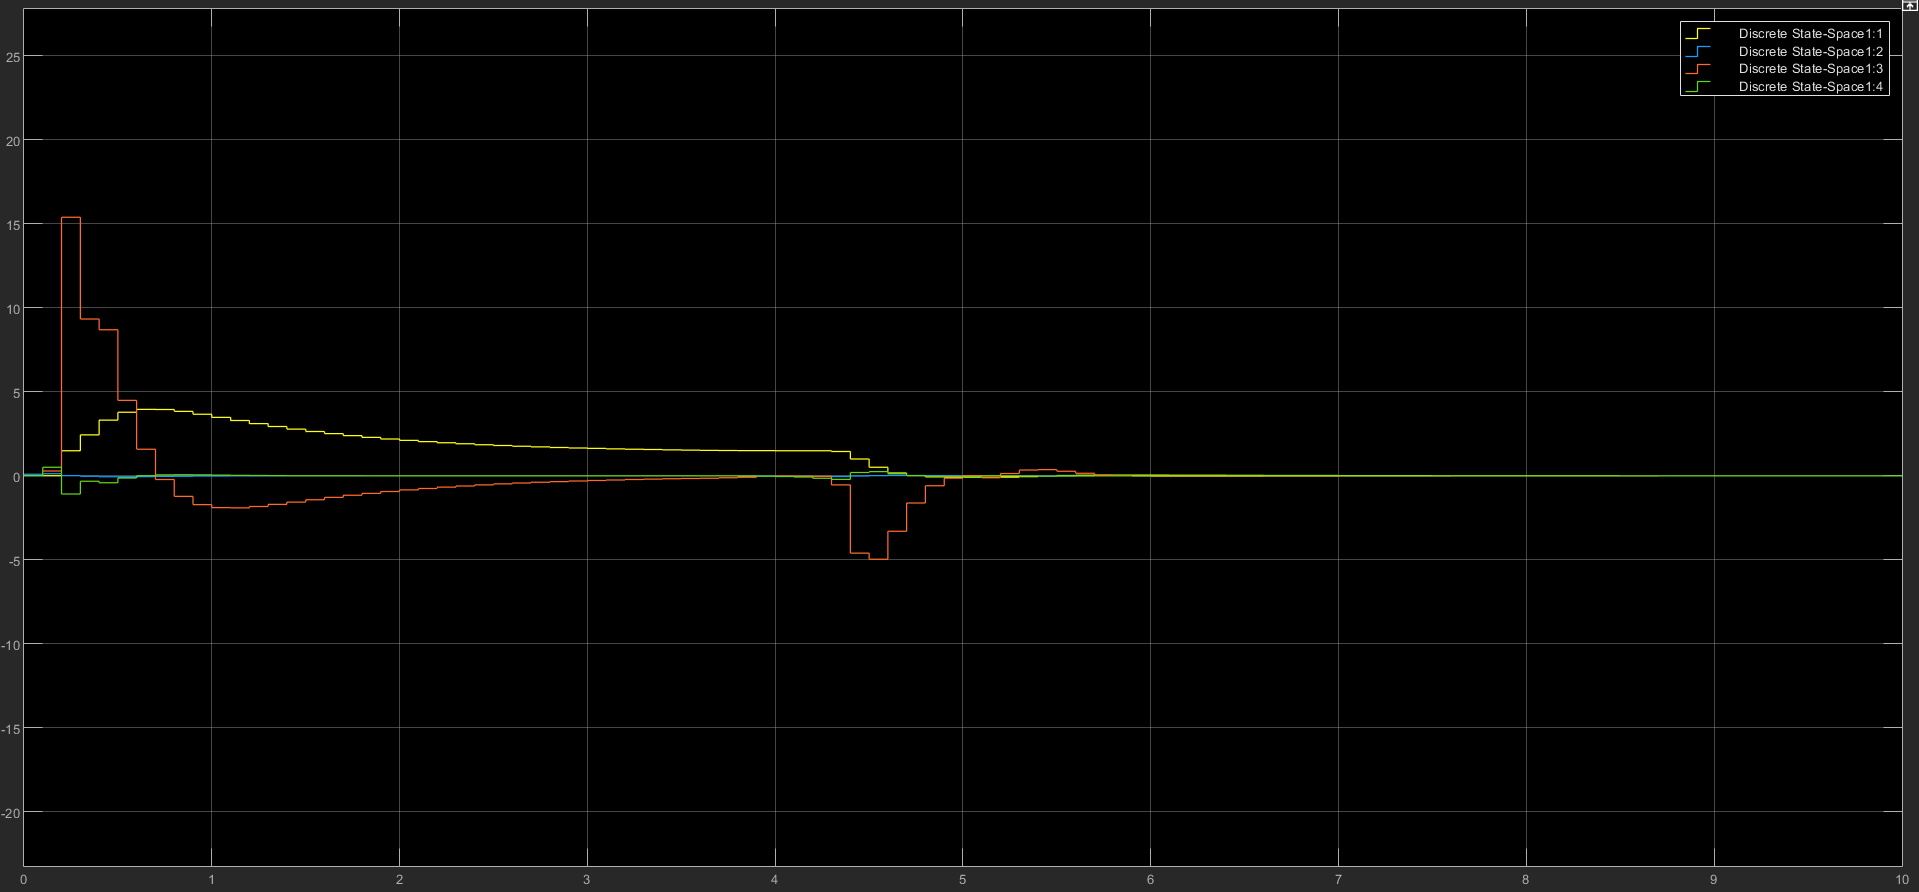
\includegraphics[width=1\linewidth]{../img/Q4_Soft_output}
	\caption{پاسخ کنترلر MPC محدود با قید های نرم}
	\label{fig:q4softoutput}
\end{figure}

\begin{figure}[H]
	\centering
	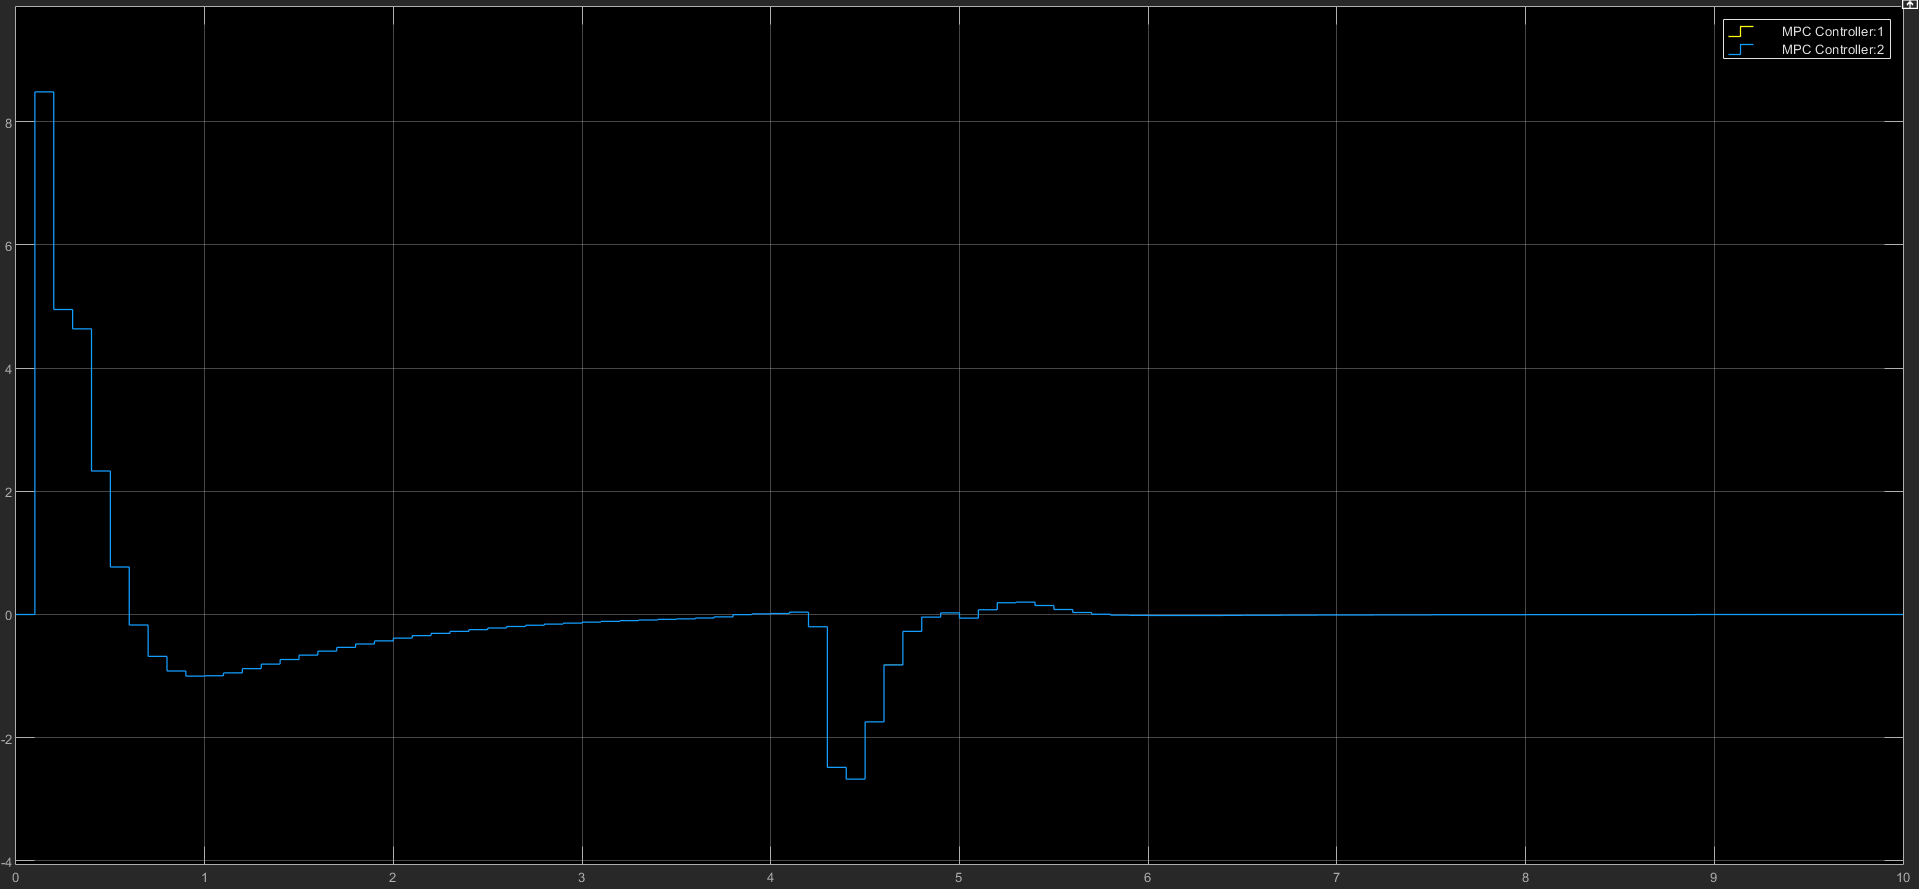
\includegraphics[width=1\linewidth]{../img/Q4_Soft_control_effort}
	\caption{تلاش کنترلی کنترلر MPC با قید های نرم}
	\label{fig:q4softcontroleffort}
\end{figure}

\subsection{بخش پنجم}
\subsubsection{نرم}
با تنظیم محدودیت ها و اجرای برنامه در حالت نرم خواهیم داشت:

\begin{figure}[H]
	\centering
	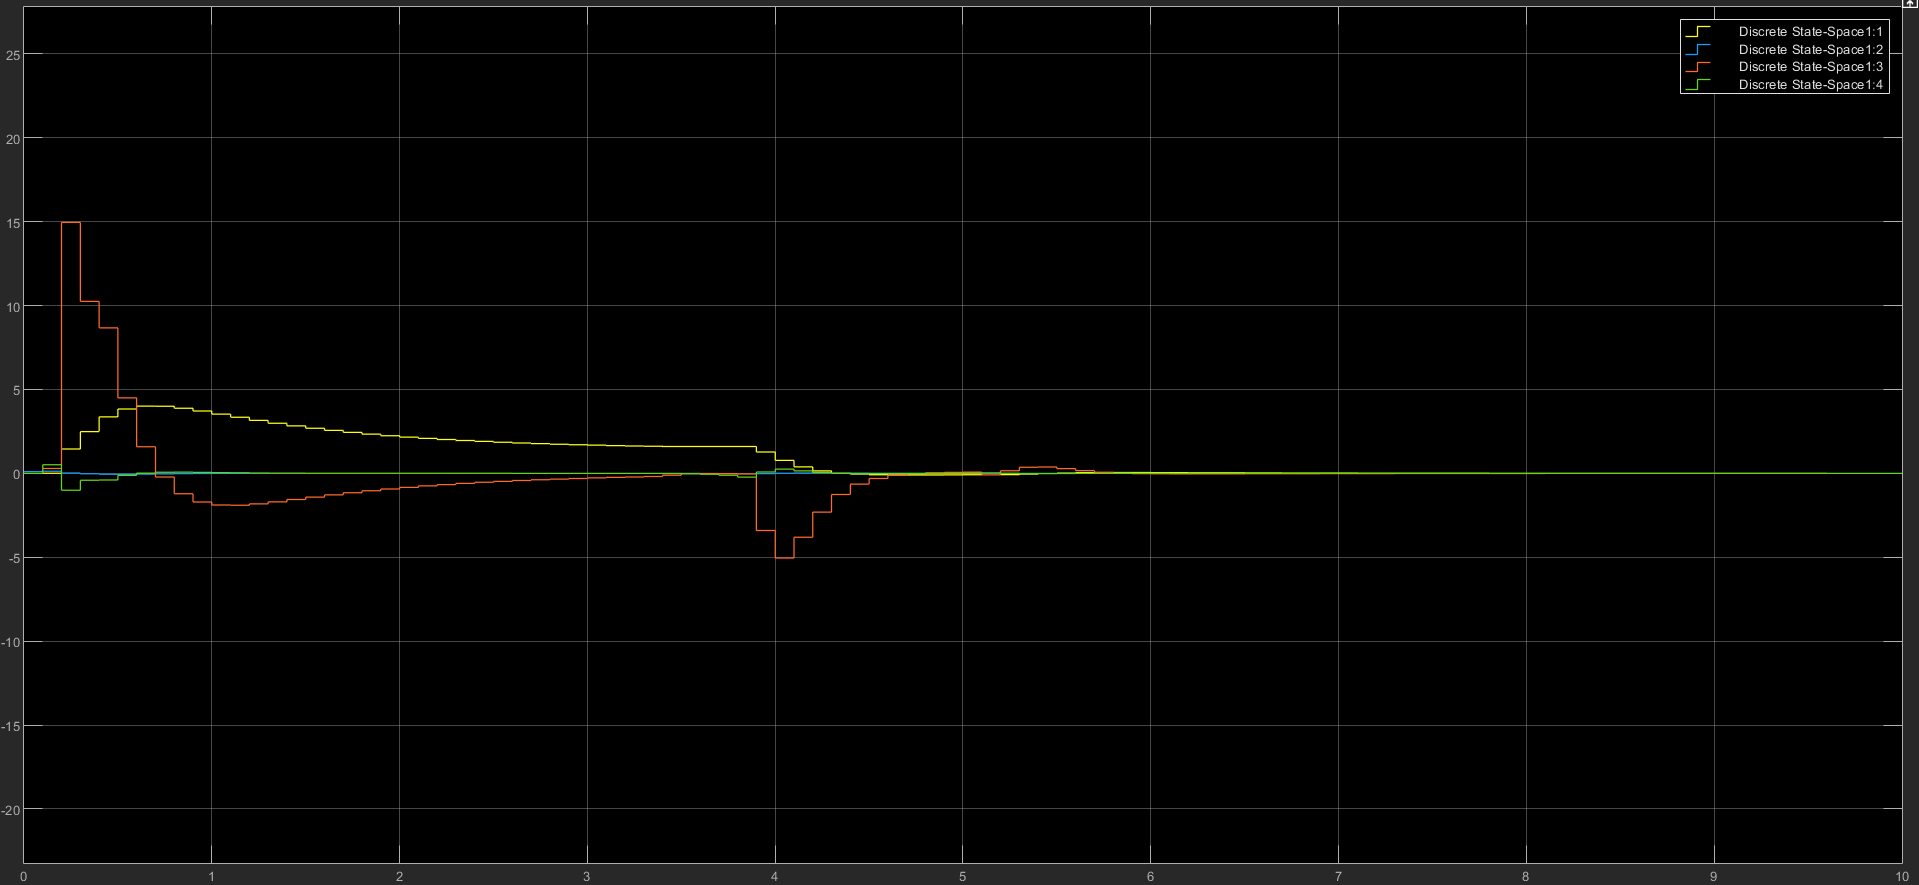
\includegraphics[width=1\linewidth]{../img/Q5_Soft_output}
	\caption{تلاش کنترلی کنترلر MPC با قید های نرم}
	\label{fig:q5softoutput}
\end{figure}

\begin{figure}[H]
	\centering
	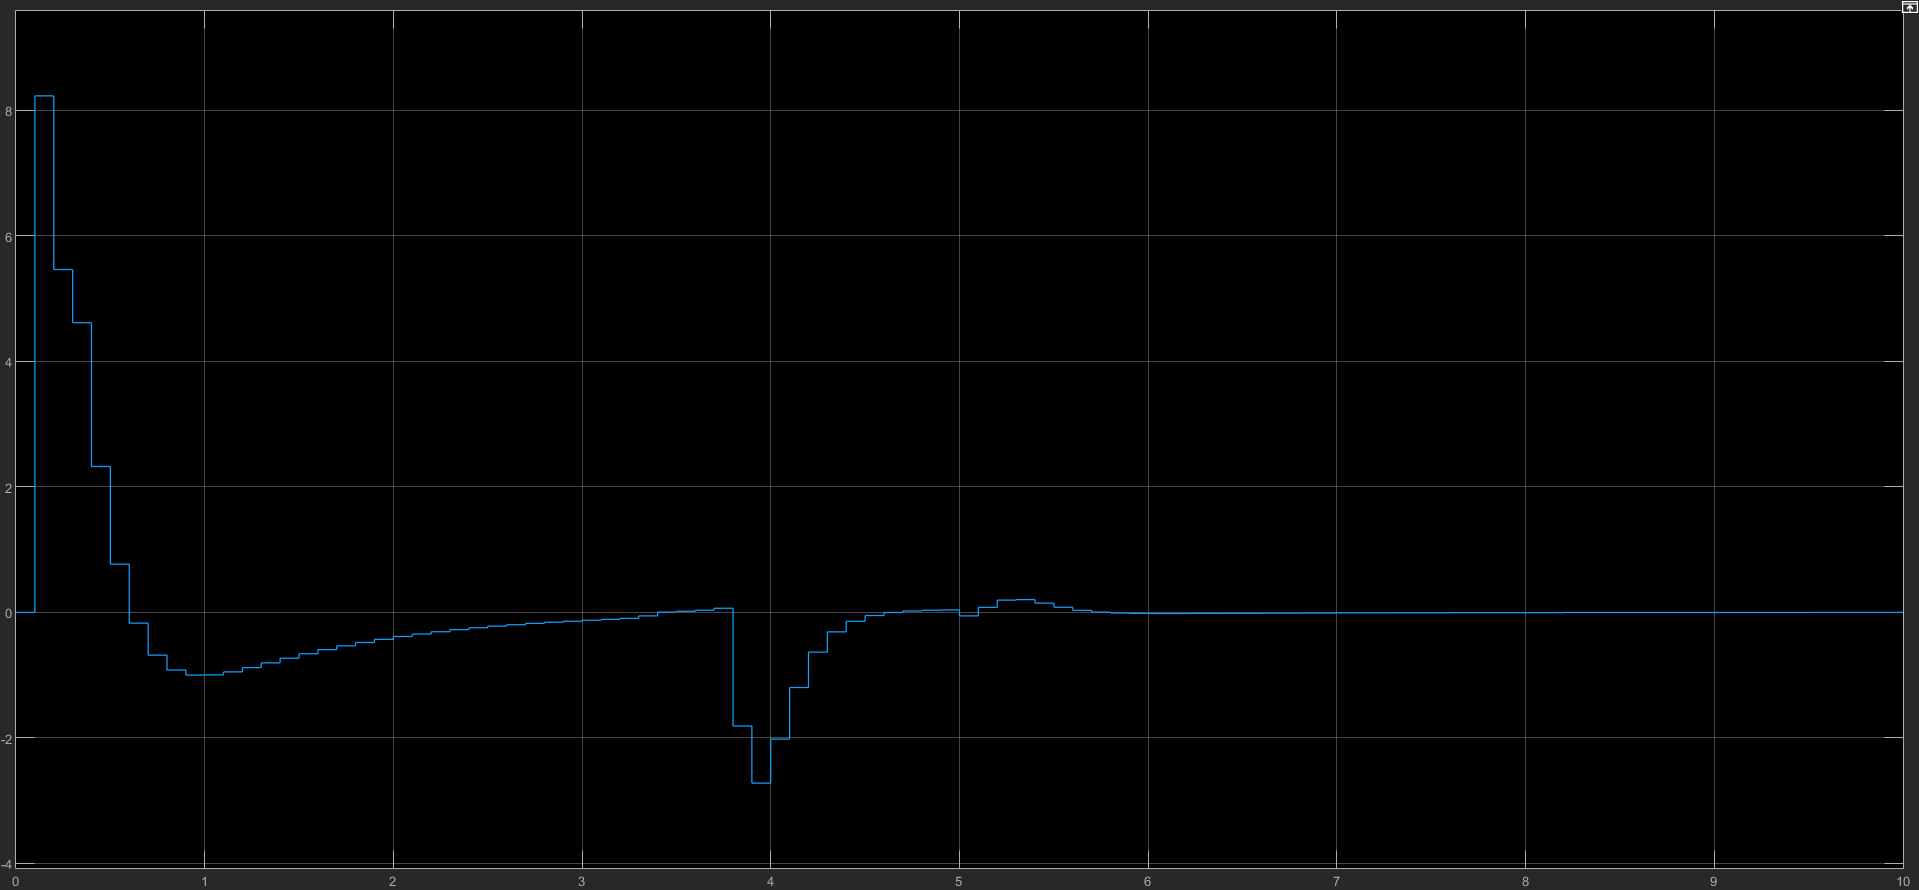
\includegraphics[width=1\linewidth]{../img/Q5_Soft_control_effort}
	\caption{پاسخ کنترلر MPC محدود با قید های نرم}
	\label{fig:q5softcontroleffort}
\end{figure}

\subsubsection{سخت}
با تنظیم محدودیت ها و اجرای برنامه در حالت سخت خواهیم داشت:

\begin{figure}[H]
	\centering
	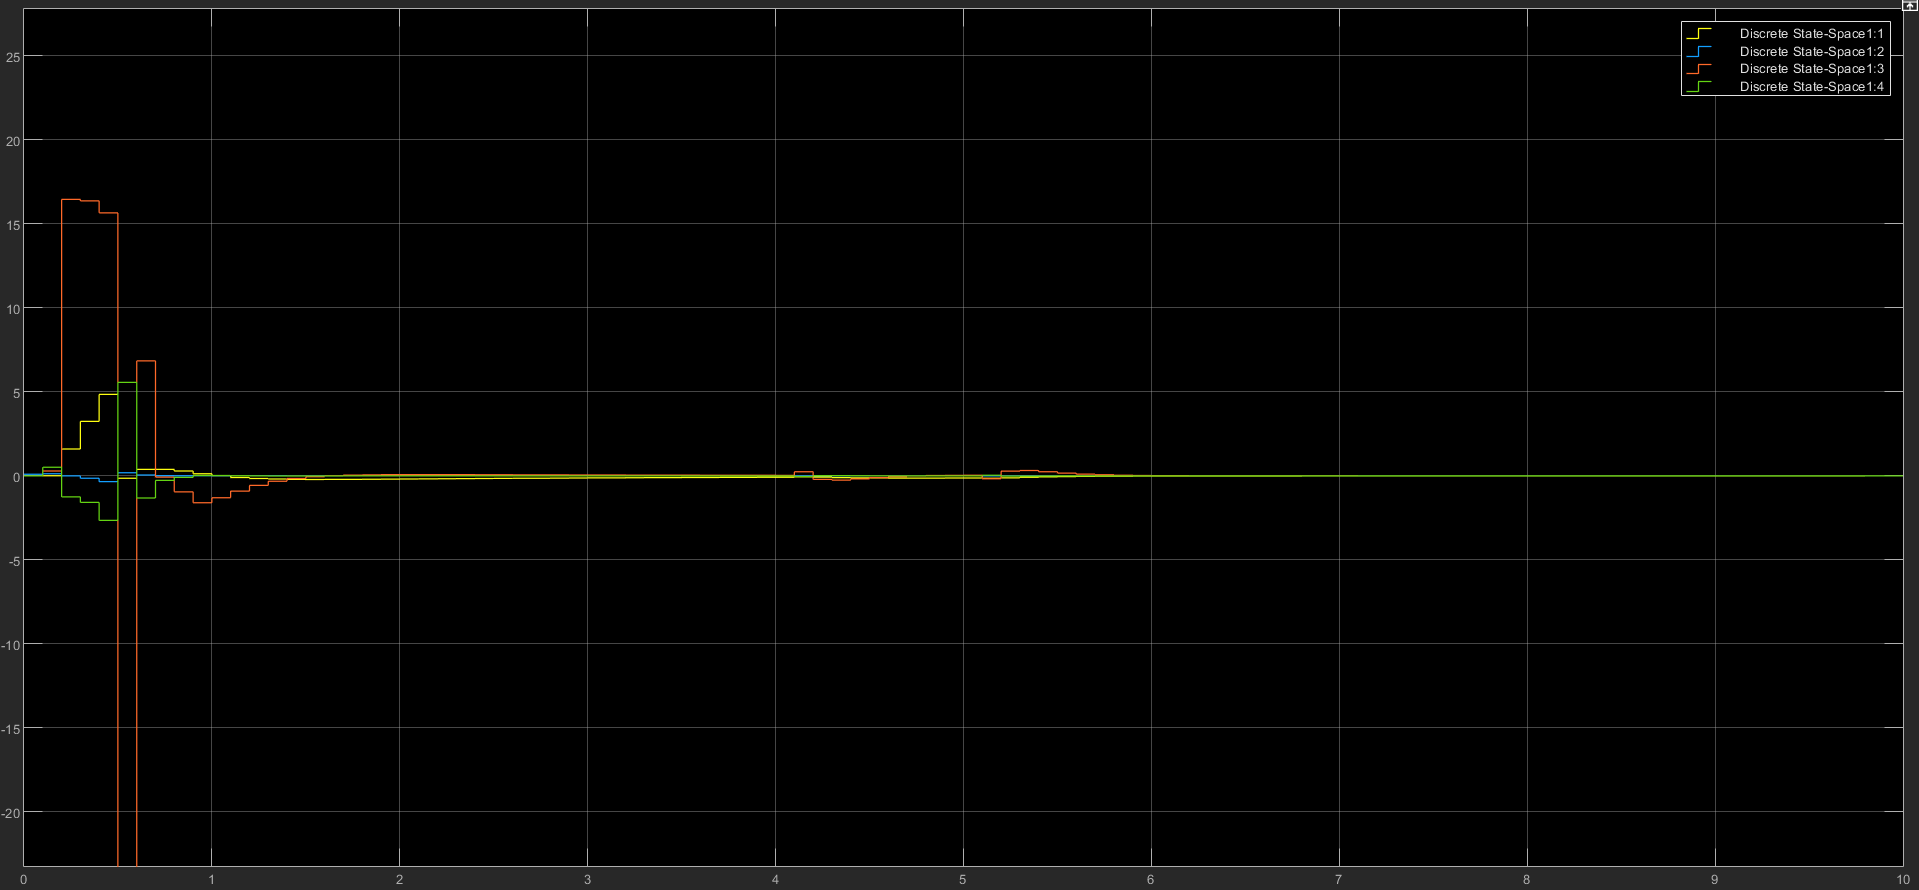
\includegraphics[width=1\linewidth]{../img/Q5_Hard_output}
	\caption{پاسخ کنترلر MPC محدود با قید های سخت}
	\label{fig:q5hardoutput}
\end{figure}

\begin{figure}[H]
	\centering
	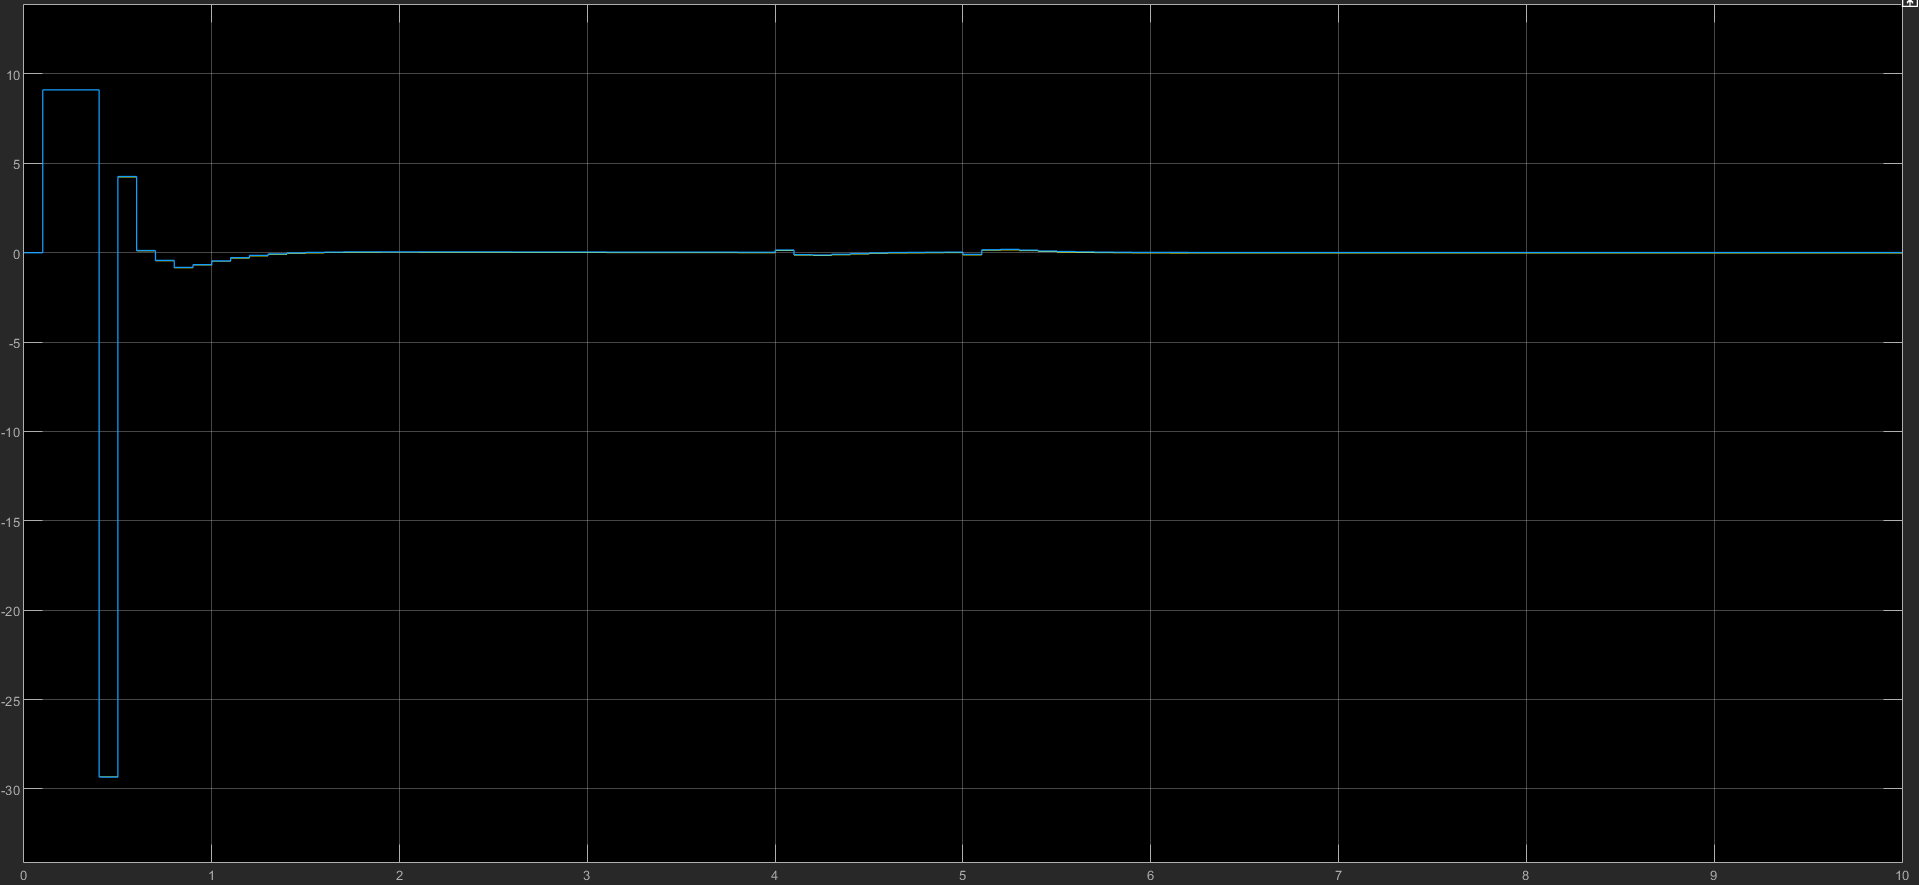
\includegraphics[width=1\linewidth]{../img/Q5_Hard_control_effort}
	\caption{پاسخ کنترلر MPC محدود با قید های سخت}
	\label{fig:q5hardcontroleffort}
\end{figure}



 
 
 
 
 
 
 
 
 
 
 		% فصل اول: مقدمه
%% !TeX root=../main.tex
\setcounter{topnumber}{5}      % Increase number of floats at the top of the page
\setcounter{totalnumber}{5}    % Increase total number of floats on a page
\renewcommand{\floatpagefraction}{.8}  % Allow more of the page to be taken up by floats

\chapter{مروری بر مطالعات انجام شده}
%\thispagestyle{empty} 
\section{مقدمه}
در این فصل، پژوهش‌های پیشین در زمینه‌ی موتورهای صفحه‌ای مبتنی بر شناوری مغناطیسی (MLPM) با تمرکز بر ویژگی‌های اساسی آنان که به طور کلی در بخش‌های زیر دسته‌بندی شده‌اند، مورد بررسی قرار می‌گیرند. 

	\textbf{\textit{طراحی کنترلر}:}
	معرفی روش‌های کنترل کلاسیک و مدرن برای این سیستم‌ها و چگونگی بهبود پایداری و دقت حرکت.


در بخش‌های بعد، پژوهش‌های انجام‌شده بر اساس این ویژگی‌ها ارزیابی شده و مزایا و معایب هر روش مورد بررسی قرار می‌گیرد.

\section{معماری دستگاه‌های MLPM}
سیستم‌های شناوری مغناطیسی به دلیل ماهیت ناپایدارشان بدون استفاده از حلقه‌های کنترلی نمی‌توانند پایداری لازم را فراهم کنند. به همین دلیل، در تمامی ساختارهای پیشنهادی، از سیم‌پیچ‌های الکتریکی برای تولید میدان مغناطیسی با شدت کنترل ‌شده استفاده می‌شود. این سیم‌پیچ‌ها وظیفه دارند تا موقعیت جسم معلق را پایدار کرده و آن را در حالت مطلوب نگه ‌دارند.

در طراحی موتورهای صفحه‌ای، که از دو بخش ثابت
\LTRfootnote{Stator}
و متحرک
\LTRfootnote{Mover}
تشکیل شده‌اند، امکان تغییر در طراحی و محل قرارگیری آهنرباهای الکتریکی و دائمی وجود دارد. نیروی مغناطیسی وارد بر بخش متحرک می‌تواند به‌صورت جاذبه‌ای از بالا یا دافعه‌ای از پایین اعمال شود. با این حال، در موتورهای صفحه‌ای به دلیل لزوم کم بودن فاصله میان سیم‌پیچ‌ها و اجسام معلق، اعمال نیروی جاذبه‌ای از بالا امکان‌پذیر نیست. به همین دلیل، در تمامی طراحی‌ها، نیروی مغناطیسی دافعه‌ای از سمت پایین به بخش متحرک وارد می‌شود که امکان جابه‌جایی اجسامی که بر روی آنها قرار می‌گیرند را فراهم می‌کند.

با توجه به این موارد، طراحی های متفاوتی برای ساخت دستگاه‌های MLPM ارائه می‌شود که در ادامه بررسی یک مورد از آنان خواهیم پرداخت.


\subsection{‌آهنرباهای متحرک و سیم‌پیچ‌های ثابت}

معماری که برای طراحی دستگاه‌های MLPM ارائه شده است، شامل قرار دادن سیم‌پیچ‌ها در بخش استاتور و استفاده از آهنرباهای دائمی در بخش متحرک می‌باشد. این ساختار نوین که در بسیاری از پژوهش‌ها مورد استفاده قرار گرفته، مشکلات معماری‌های پیشین مانند محدودیت جابه‌جایی متحرک ناشی از اتصالات فیزیکی و چالش‌های خنک‌کاری سیم‌پیچ‌ها را برطرف کرده و منجر به بهبود عملکرد کلی سیستم شده است.

در پژوهش 
\cite{RN7}
استاتوری با چینش سیم‌پیچ‌ها مطابق با الگوی شاه‌ماهی
\LTRfootnote{Herringbone pattern}
طراحی و پیاده‌سازی شده است. این طراحی امکان اعمال نیروی مغناطیسی به دو آهنربای دیسکی تعبیه‌شده در بخش متحرک را فراهم کرده است که دقتی در حدود 1 درجه در زوایای حرکت و 1 میلی‌متر در موقعیت متحرک به دست آورده است
\cite{RN7}
. در ادامه این پژوهش، ساختاری جدید برای بخش متحرک ارائه شده که شامل 6 آهنربای دیسکی با چینش کروی و فواصل ثابت می‌باشد. این طراحی توانسته است چرخش آزادانه متحرک را حول سه محور ممکن سازد 
\cite{RN39}.
همچنین در پژوهش 
\cite{RN62}
نیز از این چینش سیم‌پیچ‌ها استفاده شده و مطابق با شبیه‌سازی‌های ارائه شده، مزیت آنان در ایجاد میدان مغناطیسی یکنواخت‌تر در نواحی کناری سیم‌پیچ‌ها نمایش داده شده است.

\section{طراحی کنترلر}
همان‌طور که پیش‌تر اشاره شد، سیستم‌های شناوری مغناطیسی ذاتاً ناپایدار هستند و برای دستیابی به پایداری، به کنترلری با عملکرد دقیق و خطای کم نیاز است. در پژوهش‌های مختلف، از کنترلرهای گوناگونی برای این سیستم‌ها بهره گرفته شده است؛ از جمله کنترلرهای کلاسیک نظیر PID، کنترلرهای مدرن مانند کنترل مبتنی بر پیش‌بینی مدل (MPC) و همچنین مدل‌های مبتنی بر هوش مصنوعی نظیر شبکه‌های بازگشتی GRU. در این بخش، به بررسی این کنترلرها و مقایسه‌ عملکرد آنها خواهیم پرداخت.
\subsection{کنترلر PID}

کنترل تناسبی-انتگرالی-مشتقی (PID) به عنوان یکی از پرکاربردترین و موثرترین کنترلرهای کلاسیک در سیستم‌های دینامیکی، گزینه‌ای مناسب برای کنترل سیستم‌های MLPM محسوب می‌شود. این کنترلر به دلیل سادگی در پیاده‌سازی، تنظیم دقیق و توانایی تنظیم خروجی سیستم بر اساس خطاهای ورودی، به‌طور گسترده در سیستم‌های مختلف استفاده شده است. برای کنترل سیستم‌های MLPM، به ازای هر درجه آزادی یک کنترلر PID طراحی و پیاده‌سازی می‌شود تا بتواند جریان الکتریکی سیم‌پیچ‌ها را تنظیم کرده و میدان مغناطیسی لازم برای ایجاد و حفظ موقعیت متحرک را تأمین کند.

در پژوهش‌های متعددی از کنترلر PID برای سیستم‌های MLPM بهره گرفته شده است. به عنوان مثال، در 
\cite{RN39,RN24}
از کنترلرهای PID ساده برای کنترل جریان سیم‌پیچ‌ها استفاده شده که وظیفه تنظیم میدان مغناطیسی و در نتیجه، کنترل موقعیت جسم متحرک را بر عهده دارند. علاوه بر این، در پژوهش
\cite{RN32}
، از دو کنترلر PID در یک ساختار دوگانه استفاده شده است. کنترلر اول برای جابه‌جایی‌های بلند و در مسافت‌های طولانی به کار رفته و جریان سیم‌پیچ‌های اصلی را تنظیم می‌کند، در حالی که کنترلر دوم برای حرکات دقیق کوتاه‌برد طراحی شده و کنترل جریان سیم‌پیچ‌های ثانویه را بر عهده دارد. این روش باعث بهینه‌سازی کنترل دقیق و بهبود دقت در حرکات کوتاه‌برد و جابه‌جایی‌های سریع می‌شود.
همچنین در سیستم MagTable، برای کنترل دقیق موقعیت آهنرباهای دائمی، از شش کنترلر PID به‌صورت همزمان استفاده شده است تا نیروی متوازن برای پایدارسازی موقعیت متحرک در چندین جهت فراهم شود 
\cite{RN8}
. این نوع طراحی و استفاده از کنترلرهای PID نشان می‌دهد که علی‌رغم محدودیت‌های موجود در کنترلرهای کلاسیک، این روش همچنان در بسیاری از سیستم‌های مغناطیسی پیچیده مانند MLPM کارایی بالایی دارد.

\begin{figure}[ht]
	\centering{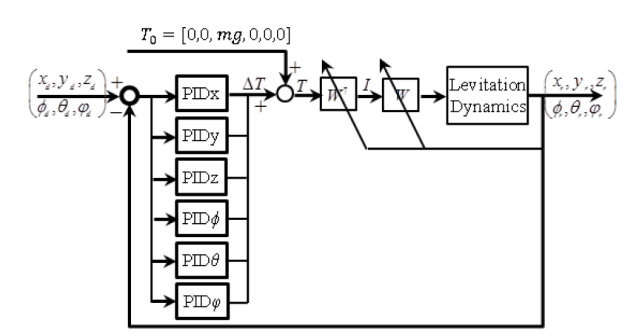
\includegraphics[width=0.5\textwidth]{PID_1}}
	\caption{کنترلر PID با 6 درجه آزادی
		\cite{RN8}}
	\label{fig:PID}
\end{figure}


\subsection{کنترلر مبتنی بر پیش‌بینی مدل MPC}
برای کنترل سیستم‌های MLPM اگر مدل سیستم به روش‌های تحلیلی و یا عددی به دست آمده و تخمین زده شده باشد، می‌توان از این مدل‌ها برای طراحی کنترلرهای پیشرفته‌تر با هدف پیش‌بینی رفتار سیستم و استفاده از آن به صورت پیش‌خور در حلقه‌ی کنترلی استفاده کرد. روش‌های تخمین مدل این سیستم‌ها در بخش‌های بعد مورد بررسی قرار می‌گیرد. در این بخش، کنترلرهای ارائه شده در پژوهش‌های دیگر ارائه می‌شود.
به دست آوردن معادلات دینامیکی سیستم و استفاده از آنها در پیش‌بینی روشی تحلیلی است که در 
\cite{RN55}
استفاده شده است و مدل کنترلی متشکل از بلوک‌های پس‌خور و پیش‌خور برای کنترل موقعیت آهنربا طراحی شده است. همچنین در 
\cite{RN62}
از یک جدول جستجو برای تعیین رفتار سیستم در نقاط مختلف فضا استفاده شده است که این جدول به عنوان پیش‌خور به مدل کنترلی داده می‌شود. در ادامه‌ی این پژوهش، با استفاده از روش‌های شناسایی سیستم، مدلی تقریبی برای رفتار سیستم در نظر گرفته شده است و با استفاده از این مدل برای پیش‌بینی رفتار سیستم‌ مدل MPC پیاده‌سازی شده است. پژوهش 
\cite{RN30}
با تمرکز بر ارائه‌ی یک مدل پیش‌بین، با استفاده از معادلات دینامیکی سیستم و همچنین روش‌پیش‌بینی حالت بی‌تاخیر، رفتار آینده‌ی سیستم را محاسبه می‌کند.
\begin{figure}[ht]
	\centering 
	\subfloat[\cite{RN55}]{
		\label{fig:MPC_1}
		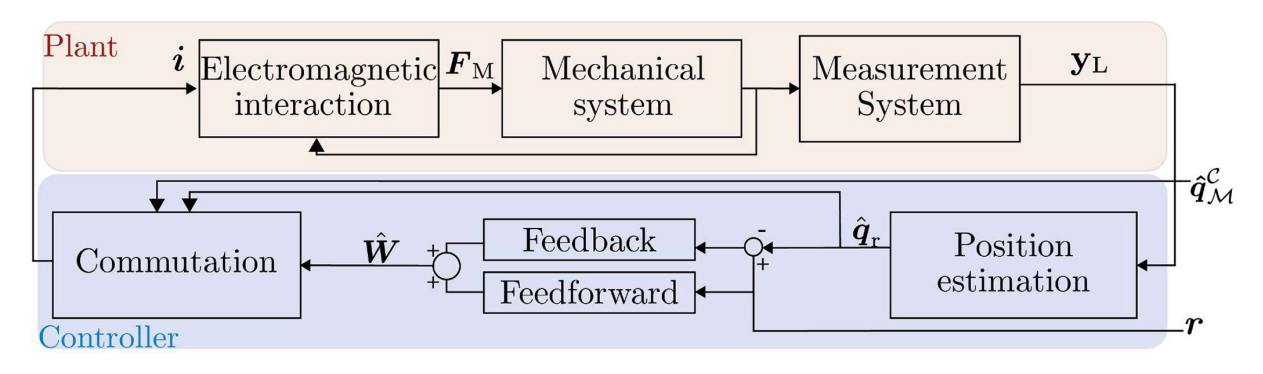
\includegraphics[width=0.45\textwidth]{MPC_1}}
	%\hspace{2mm}
	\subfloat[\cite{RN62}]{
		\label{fig:MPC_2}
		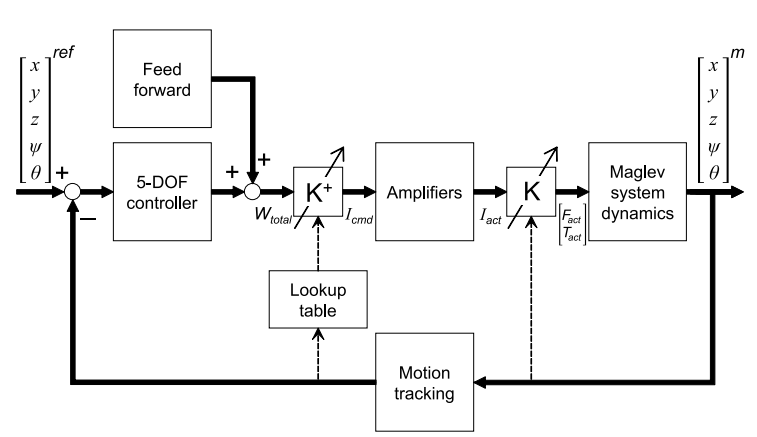
\includegraphics[width=0.45\textwidth]{MPC_2}}
	\\ % Newline to wrap the figures to the next row
	\subfloat[\cite{RN61}]{
		\label{fig:MPC_3}
		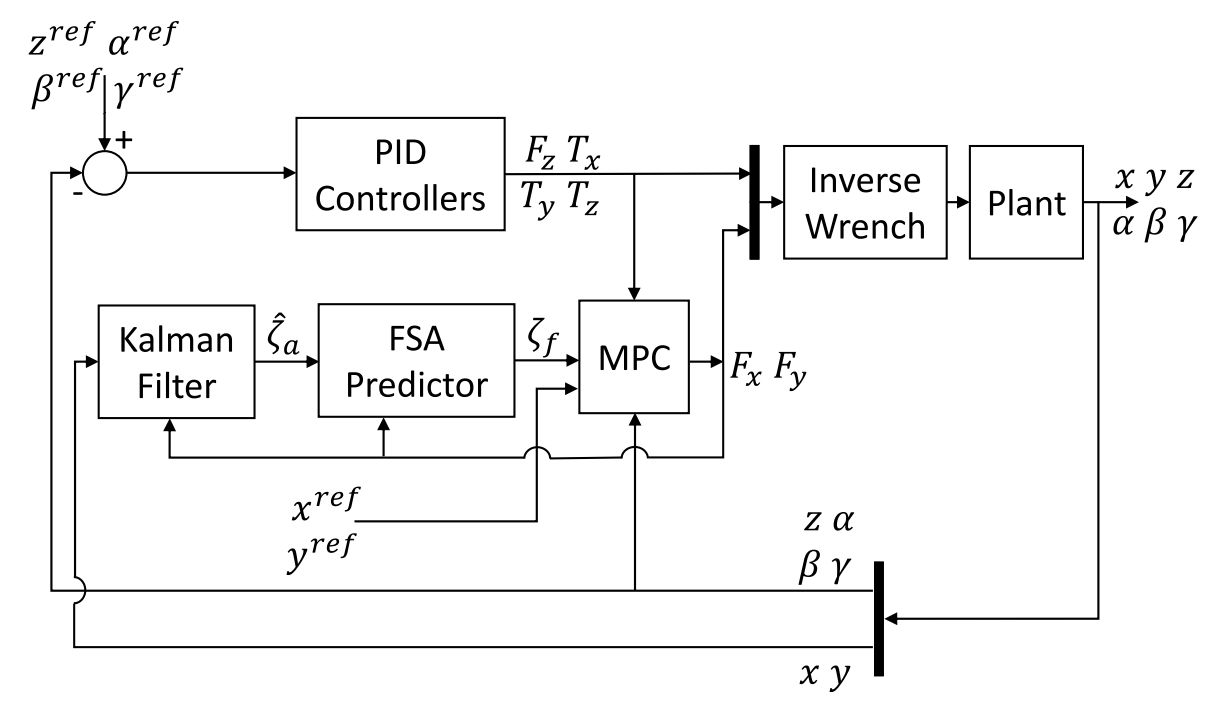
\includegraphics[width=0.45\textwidth]{MPC_3}}
	\subfloat[\cite{RN61}]{
		\label{fig:MPC_4}
		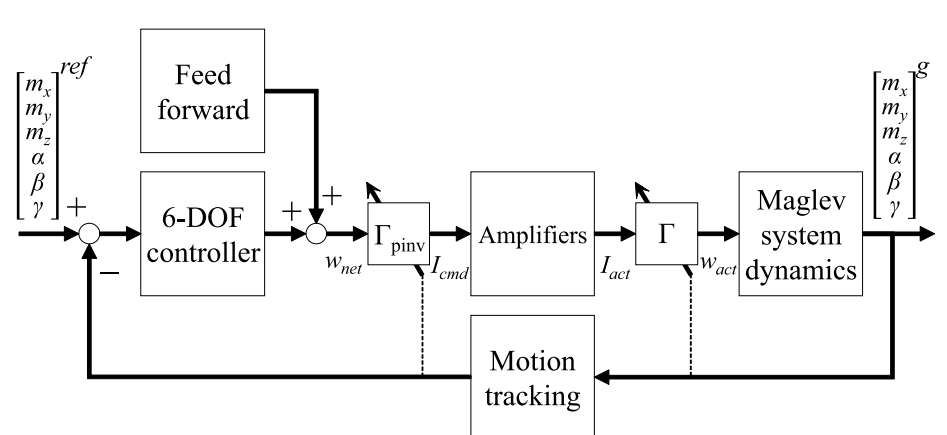
\includegraphics[width=0.45\textwidth]{MPC_4}}
	\caption{کنترلر MPC}
	\label{fig:MPC} %% label for entire figure
\end{figure}

\FloatBarrier

\subsection{کنترلر مبتنی بر هوش مصنوعی}

یکی از روش‌های نوین برای پیش‌بینی رفتار سیستم‌های پیچیده مانند MLPM، استفاده از مدل‌های هوش مصنوعی به‌ویژه شبکه‌های عصبی بازگشتی (RNN) است. این مدل‌ها با یادگیری دینامیک سیستم و ارتباط بین ورودی‌ها و خروجی‌ها، می‌توانند به‌طور مؤثری رفتار سیستم را در شرایط مختلف پیش‌بینی کنند. در این راستا، پژوهش
\cite{RN61}
از یک مدل بازگشتی GRU 
\LTRfootnote{Gated Recurrent Unit}
استفاده کرده است. این مدل بر اساس داده‌های جمع‌آوری‌شده از عملکرد دستگاه MLPM آموزش دیده و توانسته است با دقت بالا تغییرات دینامیکی سیستم و پاسخ آن به ورودی‌های گوناگون را پیش‌بینی کند. استفاده از GRU به دلیل توانایی آن در مدل‌سازی وابستگی‌های زمانی و در نظر گرفتن اطلاعات قبلی برای پیش‌بینی‌های دقیق‌تر، رویکردی مناسب در این پژوهش بوده است.(شکل 
\ref{fig:GRU}

\begin{figure}[H]
	\centering
	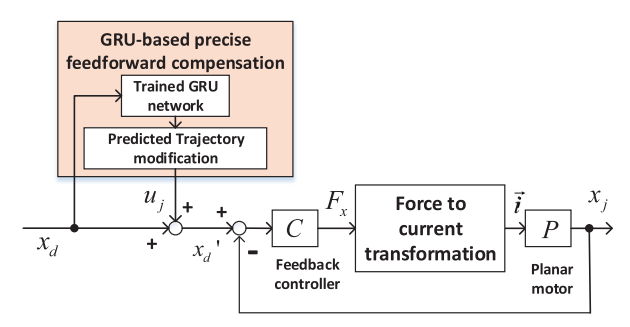
\includegraphics[width=0.5\textwidth]{GRU_1}
	\caption{کنترلر پیش‌خور GRU \cite{RN61}}
	\label{fig:GRU}
\end{figure}

\section{پروژه پیشنهادی}
با بررسی موارد ذکر شده در قسمت های پیشین، در این پژوهش تلاش می شود تا برای سیستم شناوری مغناطیسی ذکر شده در \cite{RN30} یک کنترلر مبتنی بر پیش بینی مدل طراحی و اجرا شود. مدل این سیستم در بخش بعد ذکر می شود. همچنین، حلقه ی کنترلی مورد استفاده برای این سیستم در 
\ref{fig:MPC_4}
آورده شده است.

\subsection{مدل سیستم}
سیستم مورد نظر در این پیشنهاد شامل یک محرک بدون اصطکاک و شناور در صفحه \( X_gY_g \) است. در این مدل، مقاومت هوا در تمام جهات نادیده گرفته شده و استراتژی کنترل در جهت‌های \( X_g \) و \( Y_g \) پیاده‌سازی شده است. معادلات حرکت محرک به صورت زیر بیان می‌شود:

\begin{equation}
	F_x = m a_{g_x},
	\quad F_y = m a_{g_y},
\end{equation}

که در آن \( m \) جرم محرک، و \( a_{g_x} \) و \( a_{g_y} \) شتاب‌های آن در صفحه \( X_gY_g \) هستند. از این معادلات، نمایه‌ی حالت گسسته سیستم به شکل زیر استخراج می‌شود:

\begin{equation}
	\bm{\zeta}(k + 1) = \bm{A} \bm{\zeta}(k) + \bm{B} \bm{u}(k),
\end{equation}
\begin{equation}
	\bm{\rho}(k) = \bm{C} \bm{\zeta}(k),
\end{equation}

که در آن، بردار حالت برابر است با \( \bm{\zeta} = \begin{bmatrix} m a_{g_x} & v_{g_x} & m a_{g_y} & v_{g_y} \end{bmatrix}^\top \)، ورودی نیرو برابر است با \( \bm{u} = \begin{bmatrix} F_x & F_y \end{bmatrix}^\top \)، و خروجی برابر است با \( \bm{\rho} = \begin{bmatrix} m a_{g_x} & m a_{g_y} \end{bmatrix}^\top \). در اینجا، \( \Delta T \) نشان‌دهنده‌ی دوره نمونه‌برداری و \( k \) نشان‌دهنده‌ی گام زمانی گسسته است. مقادیر \( v_{g_x} \) و \( v_{g_y} \) سرعت‌ها در سیستم مختصات جهانی هستند. ماتریس‌های نمایه حالت \( \bm{A} \)، ورودی \( \bm{B} \) و خروجی \( \bm{C} \) به صورت زیر تعریف می‌شوند:

\[
\bm{A} =
\begin{bmatrix}
	1 & \Delta T & 0 & 0 \\
	0 & 1 & 0 & 0 \\
	0 & 0 & 1 & \Delta T \\
	0 & 0 & 0 & 1 \\
\end{bmatrix},
\quad
\bm{B} =
\begin{bmatrix}
	\frac{\Delta T^2}{2m} & 0 \\
	\frac{\Delta T}{m} & 0 \\
	0 & \frac{\Delta T^2}{2m} \\
	0 & \frac{\Delta T}{m} \\
\end{bmatrix},
\quad
\bm{C} =
\begin{bmatrix}
	1 & 0 & 0 & 0 \\
	0 & 0 & 1 & 0 \\
\end{bmatrix}^\top.
\]

نیروی کنترلی و گشتاور در هر دوره‌ی نمونه‌برداری به جریان سیم‌پیچ تبدیل شده و از هم جدا می‌شوند. با حرکت محرک در مناطق مختلف، مجموعه‌های مختلفی از سیم‌پیچ‌ها برای ایجاد نیروی شناوری فعال می‌شوند. هر سیم‌پیچی که در داخل مرز مربعی به ابعاد 16 اینچ در 16 اینچ قرار گیرد که مرکز و زاویه آن با محرک هم‌راستا است، فعال می‌شود، زیرا سیم‌پیچ‌های خارج از این منطقه به سختی قادر به تولید نیرو و گشتاور هستند. این مرز با لبه‌ی سیم‌پیچ که لبه‌ی آرایه‌ی مغناطیسی را لمس می‌کند، مطابقت دارد. در هر دوره‌ی نمونه‌برداری، مختصات سیم‌پیچ‌ها در سیستم مختصات جهانی به مختصات محرک تبدیل می‌شوند. اگر مرکز سیم‌پیچ در این مرز قرار گیرد، این سیم‌پیچ برای فعال‌سازی انتخاب می‌شود. یک تصویر نمونه از انتخاب سیم‌پیچ در شکل 6.8 نشان داده شده است که در آن سیم‌پیچ‌های فعال با رنگ سبز مشخص شده‌اند. برای محرک و سیم‌پیچ‌های این فصل، 25 تا 36 سیم‌پیچ به طور همزمان فعال خواهند شد.

پس از شناسایی مجموعه‌ی سیم‌پیچ‌های فعال، روش گشتاور مستقیم برای جداسازی نیروی مطلوب و گشتاور به جریان کنترل اعمال می‌شود. نیروی و گشتاور فردی اعمال شده بر روی محرک با
 \( w_g_n = [F_{g_x,n}, F_{g_y,n}, F_{g_z,n}, T_{g_x,n}, T_{g_y,n}, T_{g_z,n}]^T \)
  نشان داده می‌شود، زمانی که جریان سیم‌پیچ برابر با 1 آمپر است. شاخص سیم‌پیچ \( n \) است و محدوده‌ی \( n \) بر اساس تعداد سیم‌پیچ‌های فعال به صورت پویا تغییر می‌کند. نیروی خالص و گشتاور مطلوب بر روی محرک با \( w_g_{net} = [F_{g_x,net}, F_{g_y,net}, F_{g_z,net}, T_{g_x,net}, T_{g_y,net}, T_{g_z,net}]^T \) نشان داده می‌شود. سپس نیروی مطلوب و گشتاور به مختصات محرک با استفاده از رابطه‌ی زیر تبدیل می‌شود:

\begin{equation}
	w_m_{net} = R^m_g w_g_{net}
\end{equation}

ارتباط بین نیروی و گشتاور مطلوب محرک و بردار جریان کنترل سیم‌پیچ‌ها به شکل زیر است:

\begin{equation}
	w_m_{net} = [w_m_1, w_m_2, \dots, w_m_n] [I_1, I_2, \dots, I_n]^T = \Gamma(\vec{c}_m) I,
\end{equation}

که در آن \( \Gamma(\vec{c}_m) \) شامل تمام عناصر نیرو و گشتاور از هر سیم‌پیچ در ورودی جریان 1 آمپر است. حرکت شش درجه‌ی آزادی (DOF) همیشه به طور بیش‌ازحد فعال می‌شود. جریان کنترلی به سیم‌پیچ‌ها با استفاده از وارون مورس-پنروز محاسبه می‌شود تا مصرف انرژی به حداقل برسد. معادله‌ی جریان کنترلی به صورت زیر است:

\begin{equation}
	I = \Gamma^T (\Gamma \Gamma^T)^{-1} w_m_{net}.
\end{equation}

دامنه‌ی حرکت محرک به راحتی با افزایش آرایه‌ی سیم‌پیچ قابل افزایش است که از طریق استفاده از استراتژی پیشنهادی انتخاب سیم‌پیچ فعال و روش جداسازی جریان تحقق می‌یابد. در هنگام ساخت ماتریس نیرو و گشتاور \( \Gamma \)، مختصات اندازه‌گیری‌شده‌ی سیم‌پیچ‌ها مورد استفاده قرار می‌گیرد. خطای موقعیت سیم‌پیچ از ساختار نصب می‌تواند در این فرآیند لحاظ شود.
		% فصول دوم: مروری بر مطالعات انجام شده
%% !TeX root=../main.tex

\chapter{پاسخ سوالات سری سوم}

% دستور زیر باعث عدم‌نمایش شماره صفحه در اولین صفحهٔ این فصل می‌شود.
%\thispagestyle{empty}
\section*{ پاسخ سوال 1}
\subsection*{سوال یکم}

تابع تبدیل سیستم به صورت زیر داده شده است:
\[
\frac{K_s \,k_e \,k_{\textrm{sp}} \,{\left(A_0 +A_i \right)}}{{\left(s\,\tau +1\right)}\,{\left(s\,{A_0 }^2 +s\,{A_i }^2 +{\left(K_p +C\,s\right)}\,{\left(m_a \,s^2 +d\,s+k_e \right)}\right)}}
\]
برای محاسبه ی معادلات حالت این سیستم، از روش تحقق مینیمال استفاده می شود. لازم به ذکر است که این تبدیل به وسیله ی تابع$ tf2ss$ امکان پذیر نیست، چرا که در محاسبه ی آن مقادیر نمادین مورد استفاده قرار گرفته اند. 
برای محاسبه به روش تحقق مینیمال، ابتدا لازم است صورت و مخرج تابع تبدیل به صورت چند جمله ای مرتب در آید.
بنابراین خواهیم داشت:
\[
C_{\textrm{num}} = K_s \,k_e \,k_{\textrm{sp}} \,{\left(A_0 + A_i \right)}
\]
\[
\tiny
C_{\textrm{den}} = \left(\begin{array}{ccccc} 
	K_p \,k_e  & {A_0 }^2 + {A_i }^2 + C \,k_e + K_p \,d + K_p \,k_e \,\tau & C \,d + K_p \,m_a + \tau \,{\left({A_0 }^2 + {A_i }^2 + C \,k_e + K_p \,d \right)} & C \,m_a + \tau \,{\left(C \,d + K_p \,m_a \right)} & C \,m_a \,\tau 
\end{array}\right)
\]
طبق تعریف تحقق مینیمال ارائه شده برای این تمرین، ماتریس های حالت با تعاریف زیر محاسبه می شوند.

\[
G(s) = \frac{Y(s)}{U(s)} = \frac{\beta}{s^n + \alpha_1 s^{n-1} + \dots + \alpha_{n-1}s + \alpha_n}
\]

\[
\dot{x}(t) = 
\begin{bmatrix}
	0 & 1 & 0 & \dots & 0 \\
	0 & 0 & 1 & \dots & 0 \\
	\vdots & \vdots & \vdots & \ddots & \vdots \\
	0 & 0 & 0 & \dots & 1 \\
	-\alpha_n & -\alpha_{n-1} & -\alpha_{n-2} & \dots & -\alpha_1
\end{bmatrix}
x(t)
+
\begin{bmatrix}
	0 \\
	0 \\
	\vdots \\
	0 \\
	\beta
\end{bmatrix}
u(t)
\]
\[
y(t) = 
\begin{bmatrix}
	1 & 0 & 0 & \dots & 0
\end{bmatrix}
x(t)
\]
که در آن:
\[
\begin{aligned}
	\left\{
	\begin{aligned}
		\alpha_1 &= \frac{\left( \tau (K_p m_a + C d) + C m_a \right)}{\tau C m_a} \\
		\alpha_2 &= \frac{\left( \tau (K_p d + C k_e + A_i^2 + A_0^2) + (K_p m_a + C d) \right)}{\tau C m_a} \\
		\alpha_3 &= \frac{\left( \tau K_p k_e + (K_p d + C k_e + A_i^2 + A_0^2) \right)}{\tau C m_a} \\
		\alpha_4 &= \frac{K_p k_e}{\tau C m_a} \\
		\beta &= \frac{k_{sp} K_s k_e (A_i + A_0)}{\tau C m_a}
	\end{aligned} \right. 
\end{aligned}
\]

با این تعاریف، ماتریس های حالت به دست می آیند.
\[
A = \left(\begin{array}{cccc}
	0 & 1 & 0 & 0\\
	0 & 0 & 1 & 0\\
	0 & 0 & 0 & 1\\
	-\frac{C\,m_a \,\tau }{K_p \,k_e } & -\frac{C\,m_a +\tau \,{\left(C\,d+K_p \,m_a \right)}}{K_p \,k_e } & -\frac{C\,d+K_p \,m_a +\tau \,{\left({A_0 }^2 +{A_i }^2 +C\,k_e +K_p \,d\right)}}{K_p \,k_e } & -\frac{{A_0 }^2 +{A_i }^2 +C\,k_e +K_p \,d+K_p \,k_e \,\tau }{K_p \,k_e }
\end{array}\right)
\]

\[
B = \left(\begin{array}{c}
	0\\
	0\\
	0\\
	\frac{K_s \,k_{\textrm{sp}} \,{\left(A_0 +A_i \right)}}{K_p }
\end{array}\right)
\]

\[
C = \left[1, 0, 0, 0\right]
\]

\[
D = 0
\]
\subsection*{سوال دوم}
برای حل سوال دوم، که کنترل سیستم ذکر شده به روش MPC خطی است، لازم است ابتدا معادلات حالت این سیستم در فضای سیمولینک تعریف شوند. 
\begin{figure}[H]
	\centering
	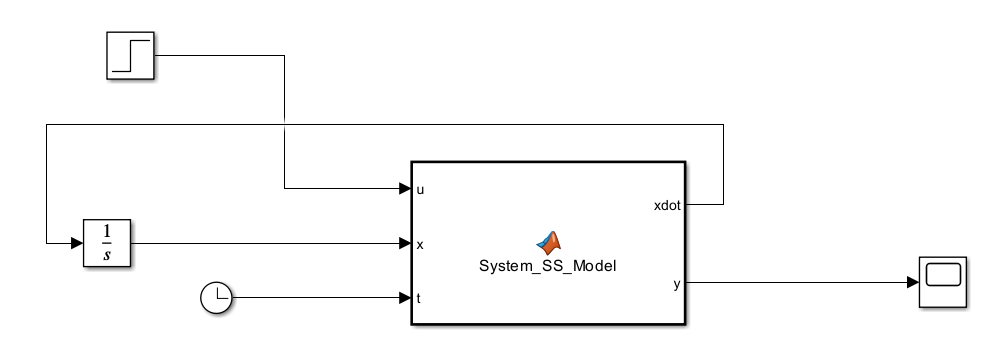
\includegraphics[width=0.7\linewidth]{../img/Q1_OL_diagram}
	\caption{دیاگرام سیستم حلقه باز در محیط سیمولینک}
	\label{fig:q1oldiagram}
\end{figure}
\begin{figure}[H]
	\centering
	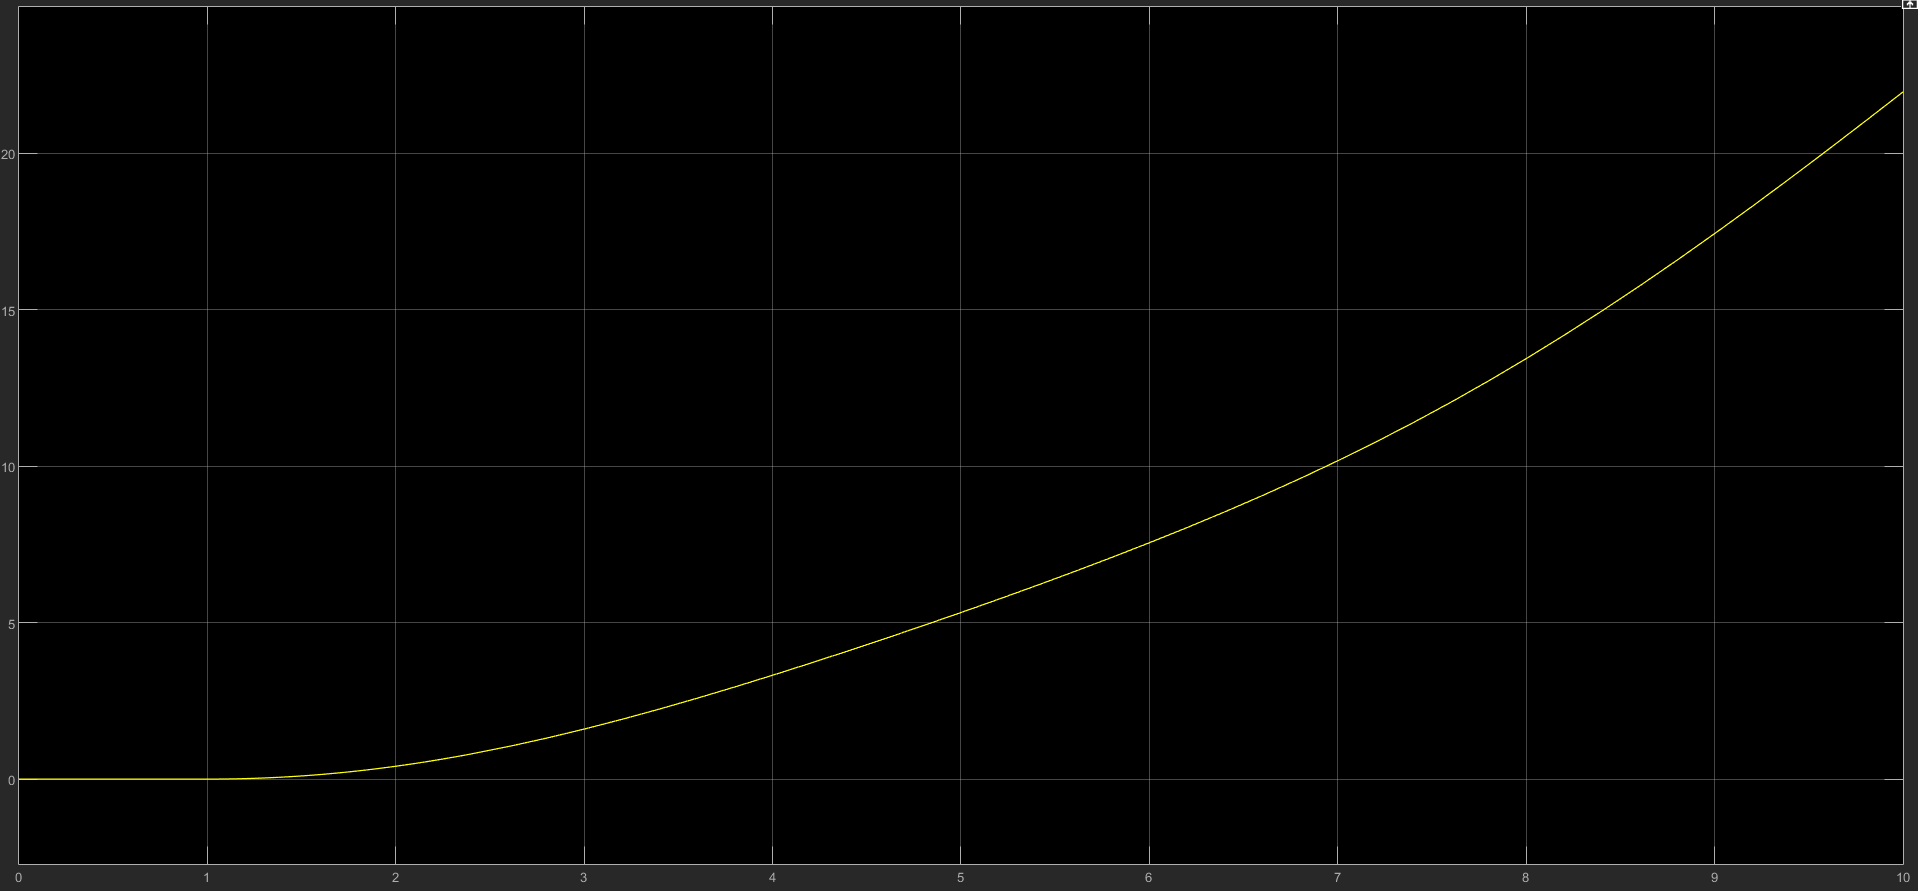
\includegraphics[width=0.7\linewidth]{../img/Q1_OL}
	\caption{پساخ حلقه باز سیستم}
	\label{fig:q1ol}
\end{figure}


همچنین، لحاظ کردن نایقینی های این سیستم در این بخش در نظر گرفته شده است. برای اعمال این نایقینی ها، از تابع سینوسی متغیر با زمان برای اعمال مقادیر انحراف از مقدار واقعی استفاده شده است.
در ادامه، با قرار دادن کنترلر MPC خطی به جای ورودی پله به این سیستم، آن را کنترل خواهیم کرد. برای تنظیم کنترلر پیش بین، از نرخ نمونه برداری 0.01 ثانیه، افق پیش بین 100 و افق کنترلی 20 استفاده شده است.
نمودار تلاش کنترلی و خروجی سیستم در نمودار زیر نمایش داده شده است.
\begin{figure}[H]
	\centering
	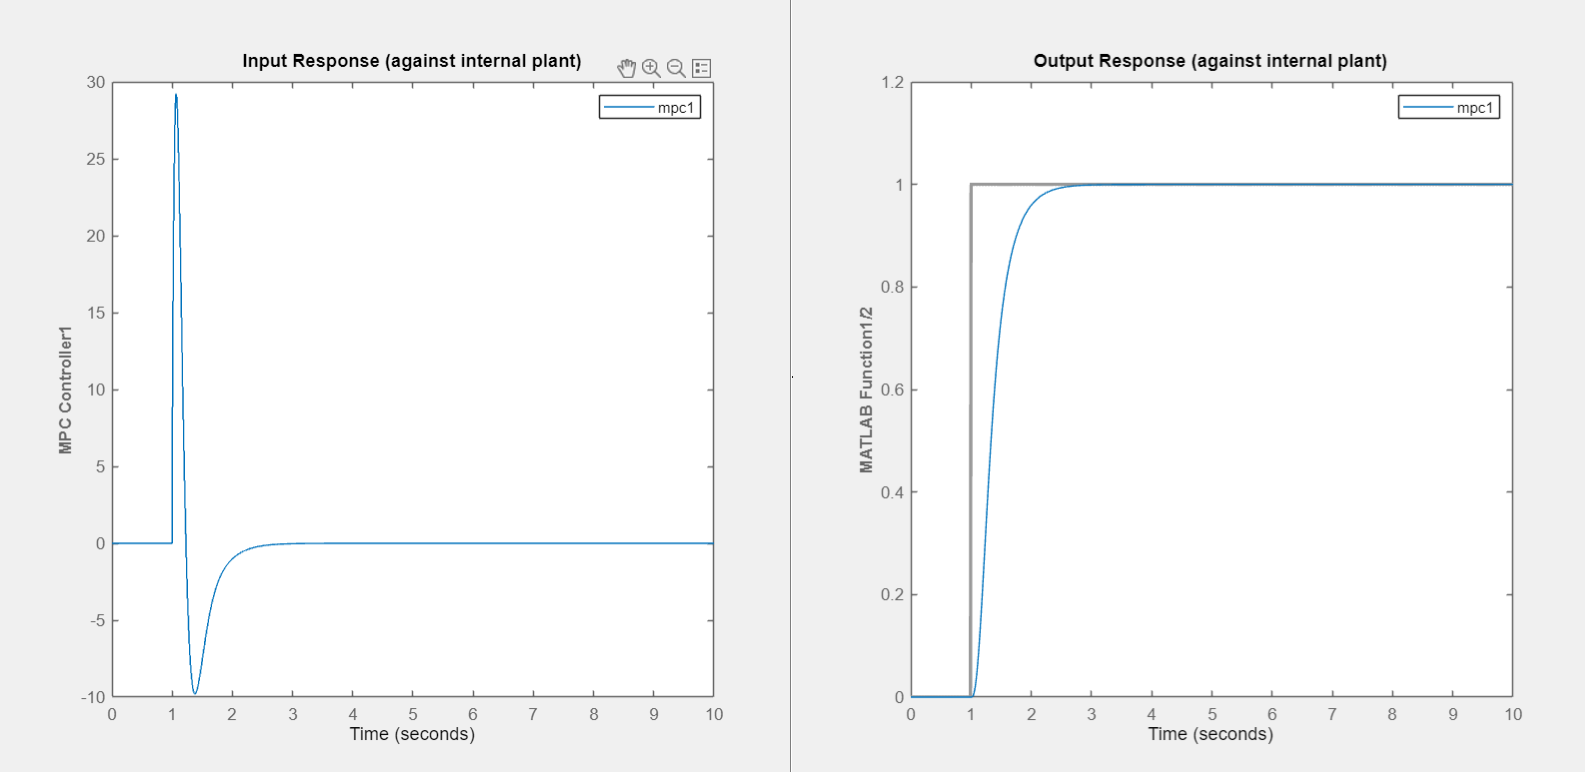
\includegraphics[width=1\linewidth]{../img/Q1_linearMPC_response}
	\caption{تلاش کنترلی و پاسخ سیستم کنترل شده با کنترلر پیش بین خطی}
	\label{fig:q1linearmpcresponse}
\end{figure}
در نتیجه پاسخ سیستم به صورت زیر به دست می آید.
\begin{figure}[H]
	\centering
	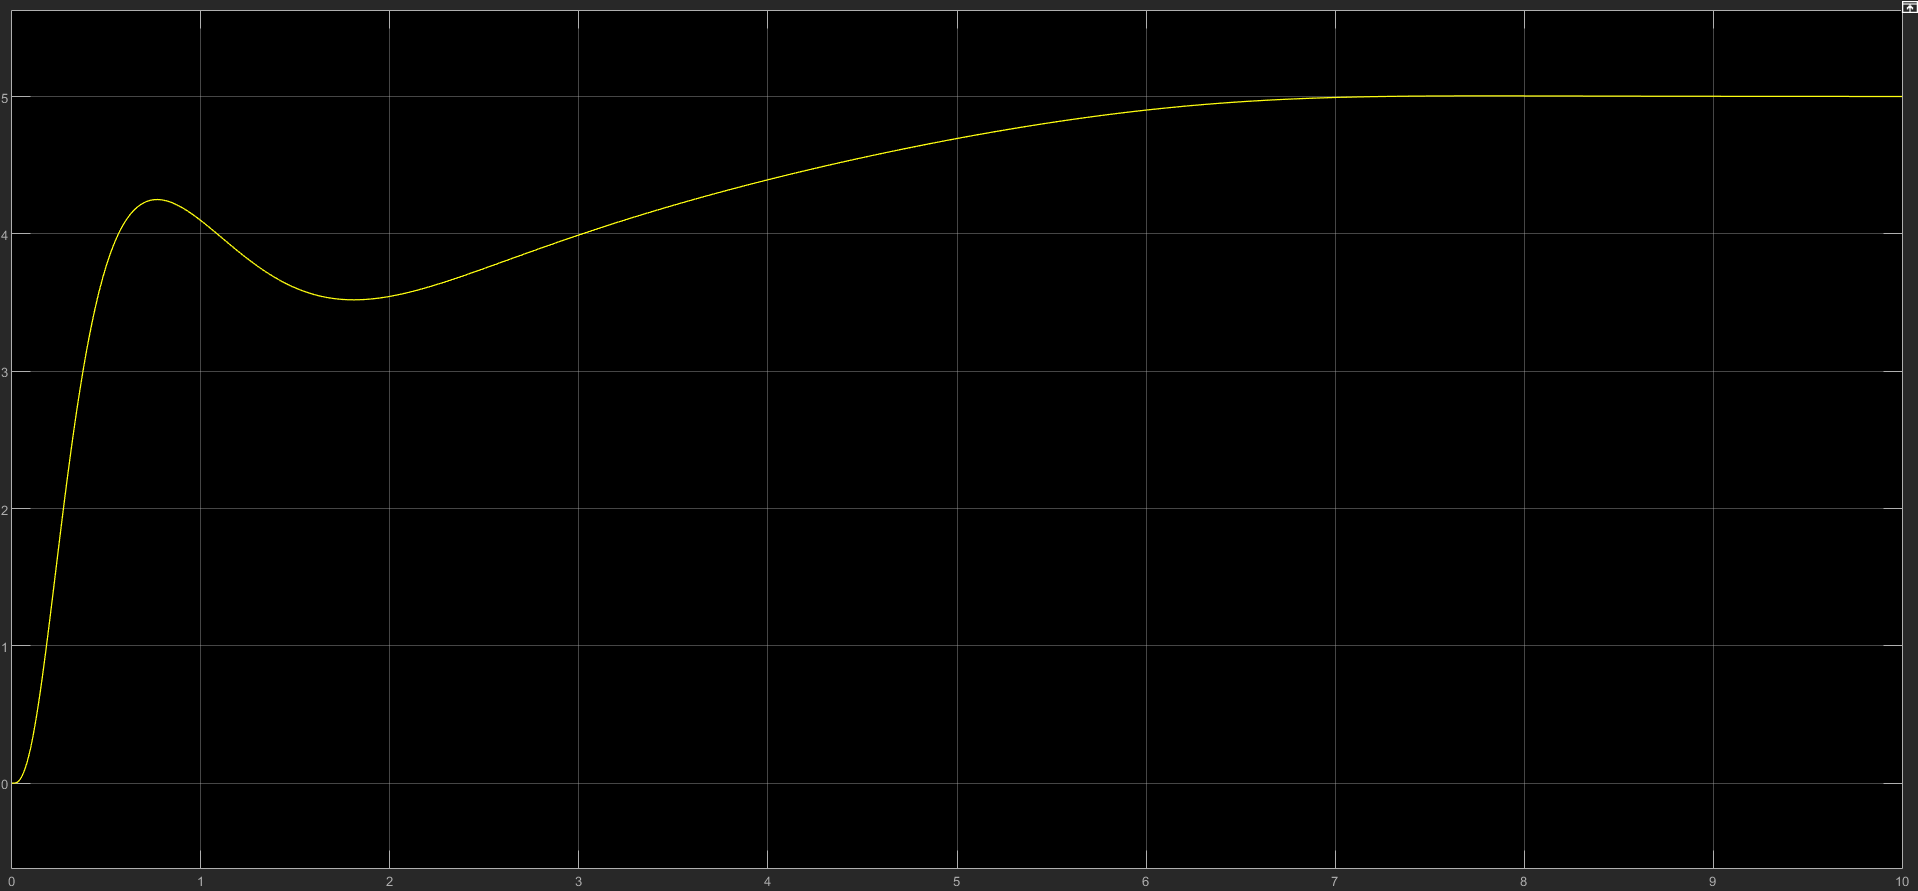
\includegraphics[width=1\linewidth]{../img/Q1_linearMPC_RES}
	\caption{پاسخ سیستم با کنترلر پیش بین خطی}
	\label{fig:q1linearmpcres}
\end{figure}

مشاهده می شود که سیستم فوق قادر است مدل را در زمان 8 ثانیه به پایداری برساند و خطای ماندگار آن صفر شود.

\subsection*{سوال سوم}
در این بخش، با اعمال اغتشاش سینوسی به سیستم، مجددا کنترلری طراحی و تنظیم می شود.
\begin{figure}
	\centering
	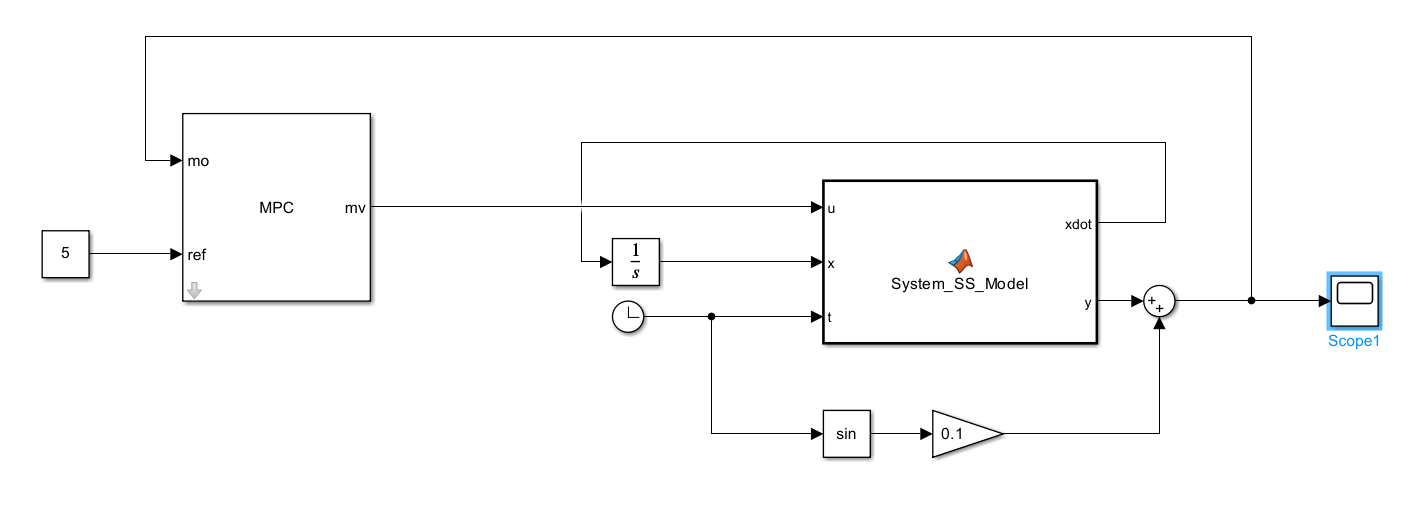
\includegraphics[width=0.7\linewidth]{../img/Q1_3_diagram}
	\caption{دیاگرام سیستم همراه با اغتشاش}
	\label{fig:q13diagram}
\end{figure}
\begin{figure}
	\centering
	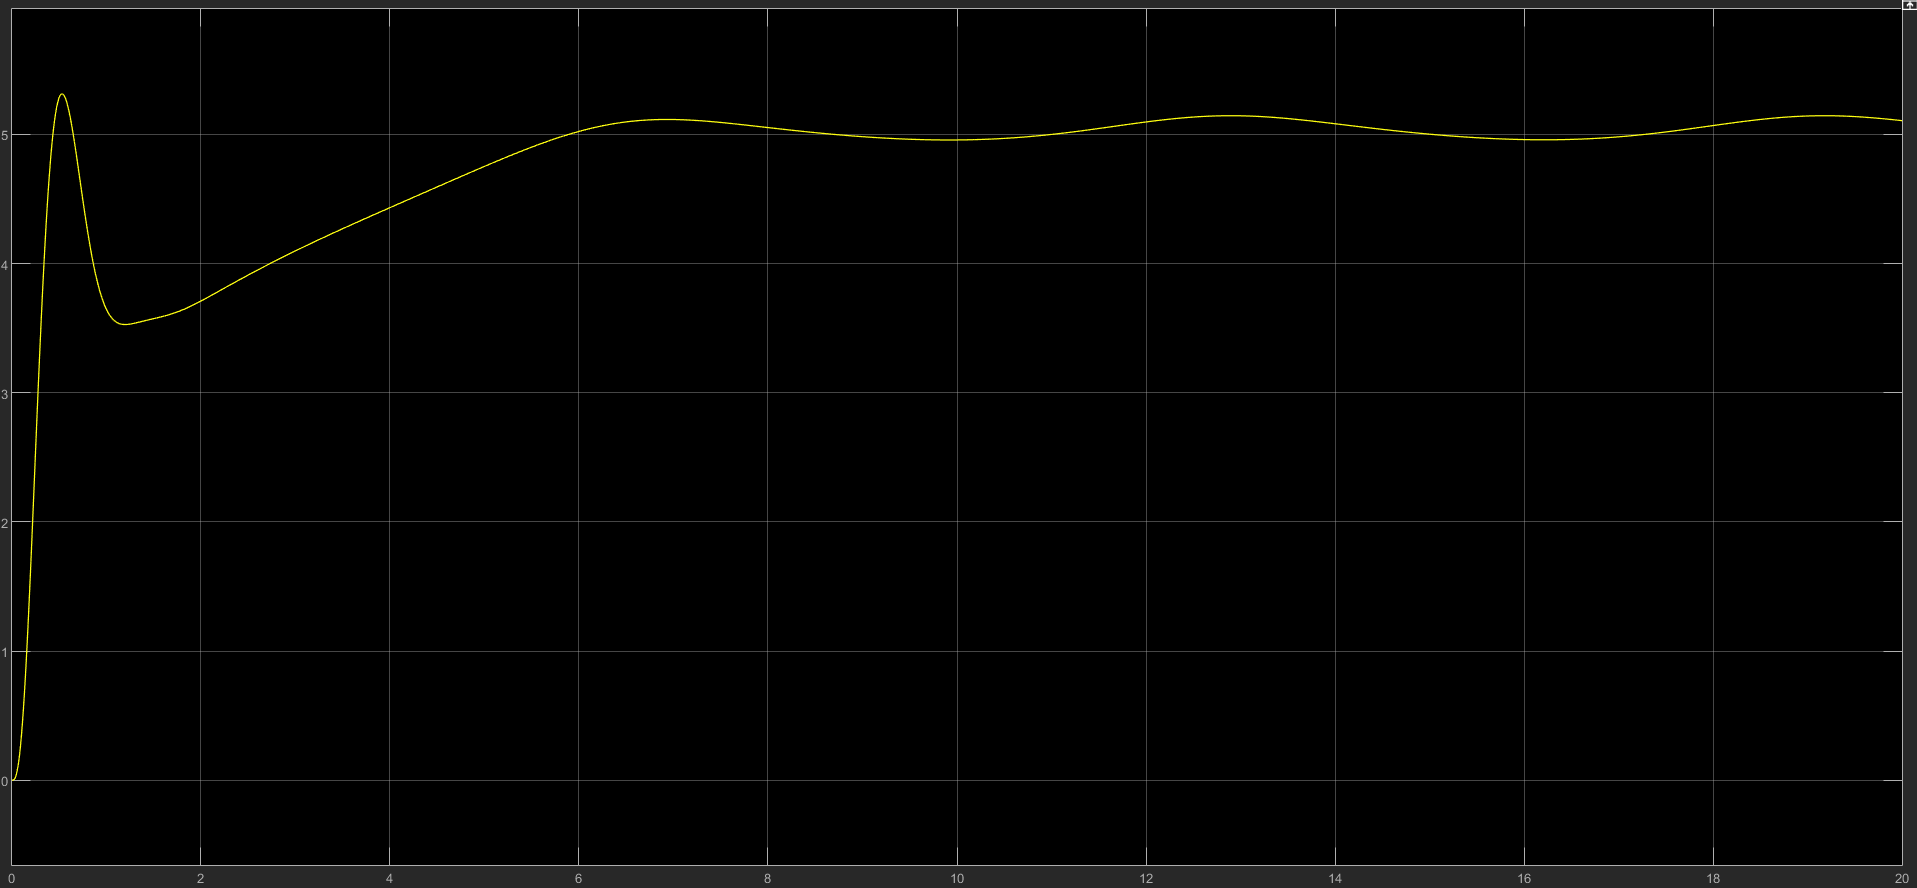
\includegraphics[width=0.7\linewidth]{../img/Q1_part3_response}
	\caption{پاسخ سیستم همراه با اغتشاش}
	\label{fig:q1part3response}
\end{figure}

مشاهده می شود که با اعمال اغتشاش به کنترلر فوق، پاسخ نهایی دارای نوسان هایی خواهد بود و این اغتشاش از سیستم حذف نشده است.
\subsection*{سوال چهارم}
در این بخش، با تغییر ساختار کنترلر به طوری که شامل یک کنترلر PID نیز باشد، سعی می کنیم تا اثر اغتشاش وارد شده به سیستم را حدف کرده و کنترلر $Tube MPC$ را تشکیل دهیم. برای این منظور، با اضافه کردن یک بلوک PID به سیستم و تنظیم ضرایب آن خواهیم داشت:
\begin{figure}[H]
	\centering
	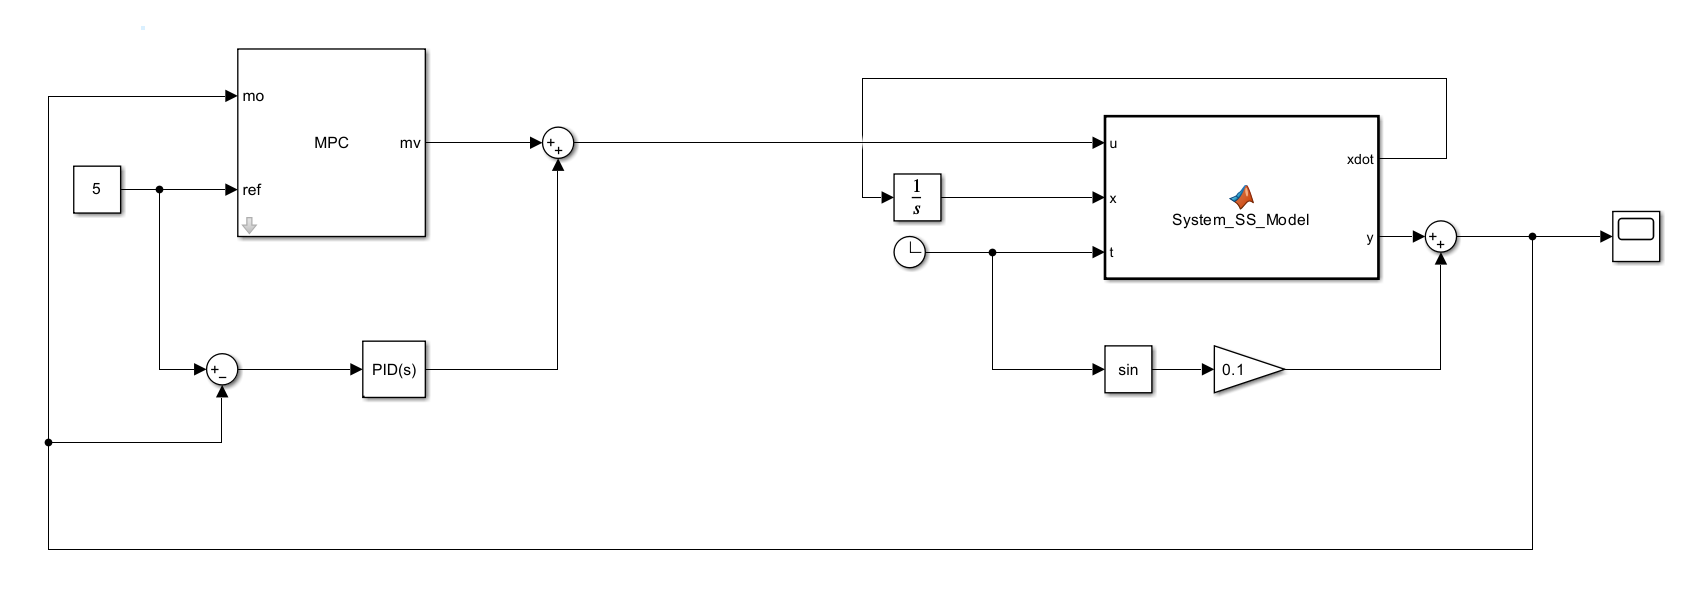
\includegraphics[width=1\linewidth]{../img/Q1_part4_diagram}
	\caption{دیاگرام سیستم $Tube MPC$}
	\label{fig:q1part4diagram}
\end{figure}
با تنظیم ضرایب PID به طوری که کنترلر بتواند با ثابت زمانی کوتاهی به تغییرات پاسخ دهد و همچنین اورشوت کمی داشته باشد تنظیم شده است.
ضرایب PID مورد استفاده در این سیستم به شرح زیر است.
\[
P = 14.05 , I = 1.12 , D = 19.04
\]
پاسخ این سیستم نسبت به ورودی قبلی به صورت زیر خواهد بود:
\begin{figure}[H]
	\centering
	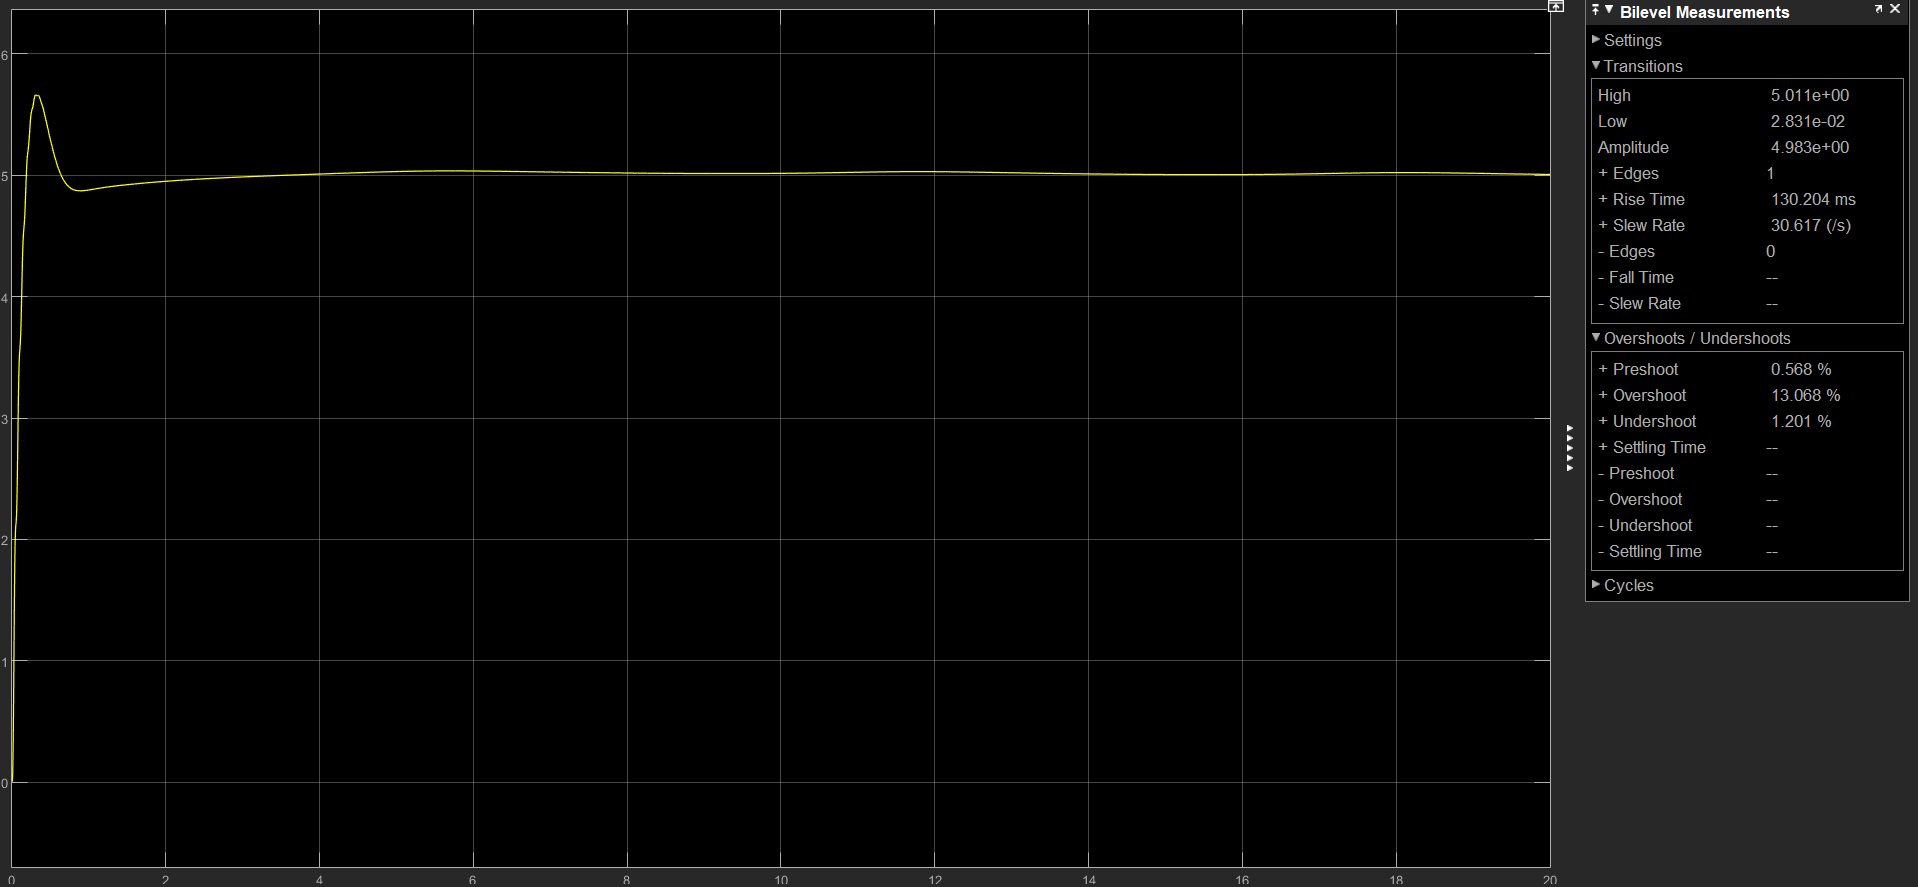
\includegraphics[width=1\linewidth]{../img/Q1_TubeMPC_Response}
	\caption{پاسخ $Tube MPC$}
	\label{fig:q1tubempcresponse}
\end{figure}
در اینجا مشاهده می شود که خطای ماندگار سیستم پس از بهینه سازی ضرایب PID، همچنان زیاد است و مقداری برابر با 13 درصد دارد که برای سیستم قابل تحمل نیست.
\subsection*{سوال پنجم}
با توجه به نتایج بخش قبل، برای کاهش میزان فراجهش، لازم است در این قسمت قیدی بر روی خروجی کنترلر اعمال شود تا از اعمال ورودی های بزرگ به سیستم خودداری شود. برای تعیین این قید، ابتدا به مشاهده و ارزیابی تلاش کنترلی کنترلر در شبیه سازی قسمت قبل می پردازیم.

\begin{figure}[H]
	\centering
	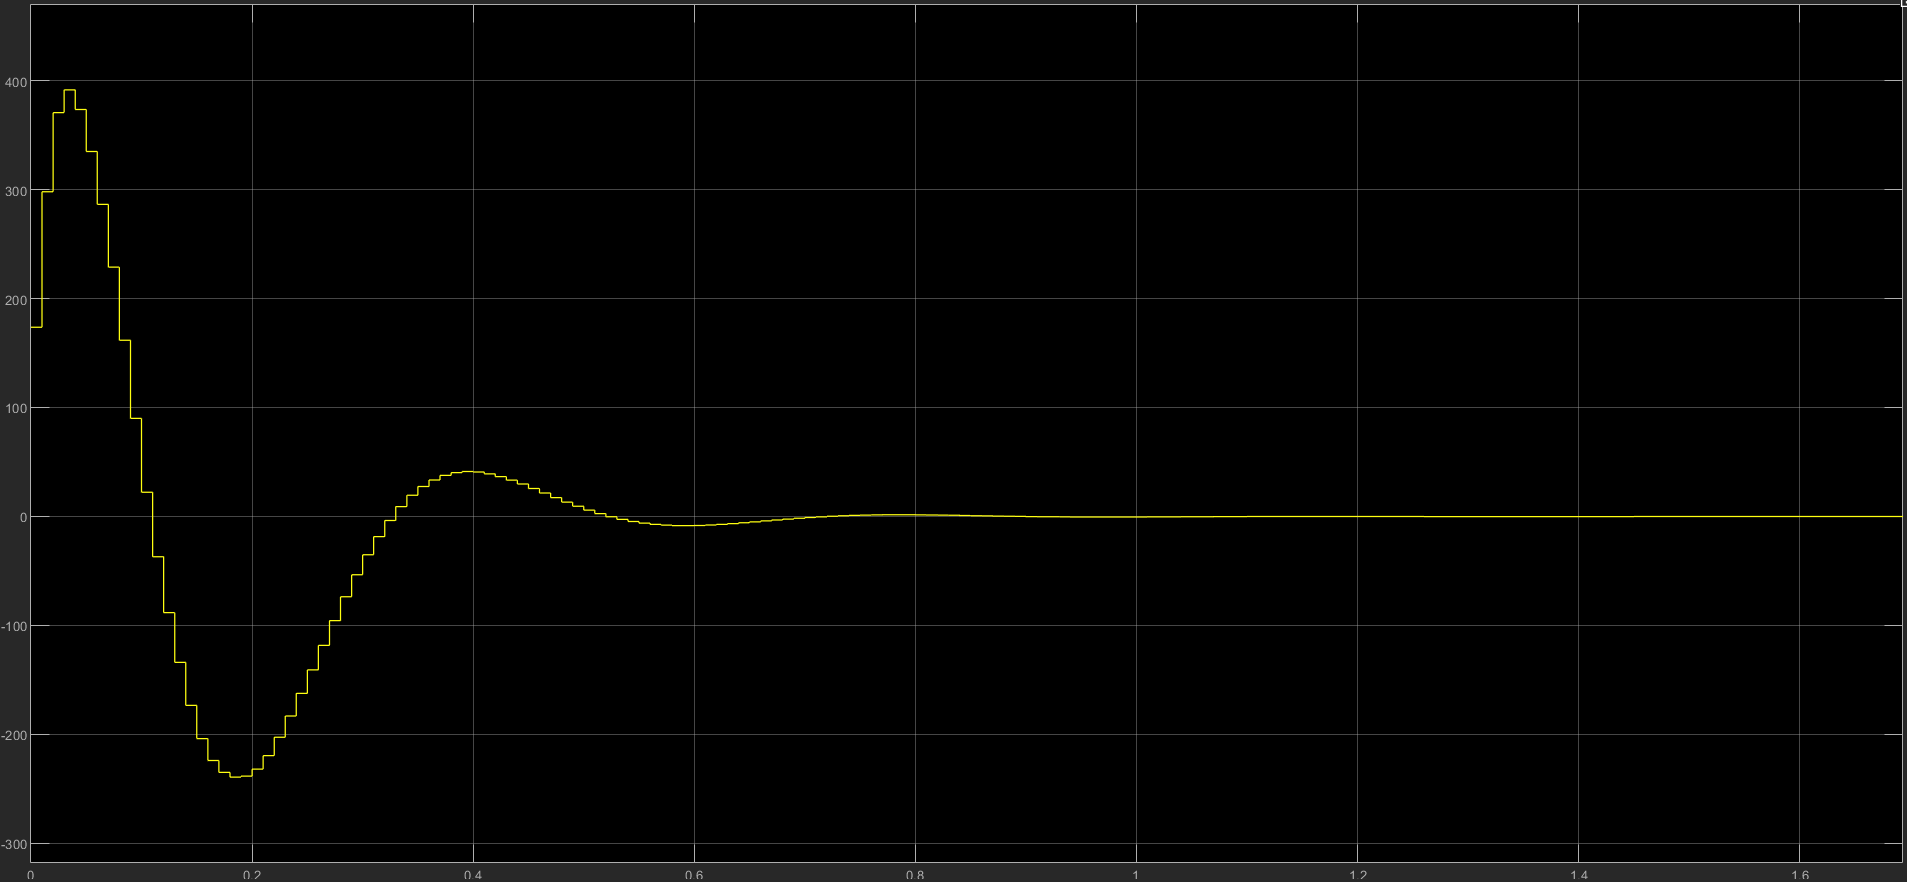
\includegraphics[width=1\linewidth]{../img/Q1_part4_Control_effort}
	\caption{تلاش کنترلی $Tube MPC$}
	\label{fig:q1part4controleffort}
\end{figure}
 
 مشاهد می شود که کنترلر فرمات های کنترلی با مقدار بیشینه ی 400 ایجاد کرده است و پس از آن، مقادیر کاهش یافته اند. با دانستن این مورد، قید هایی بر روس سیستم تنظیم شده تا بهترین نتیجه حاصل شود.
 با تنظیم مقدار فرمان کنترلی در بازه ی -10 و 10، پاسخ سیستم و تلاش کنترلی به شکل زیر به دست خواهد آمد.
\begin{figure}[H]
	\centering
	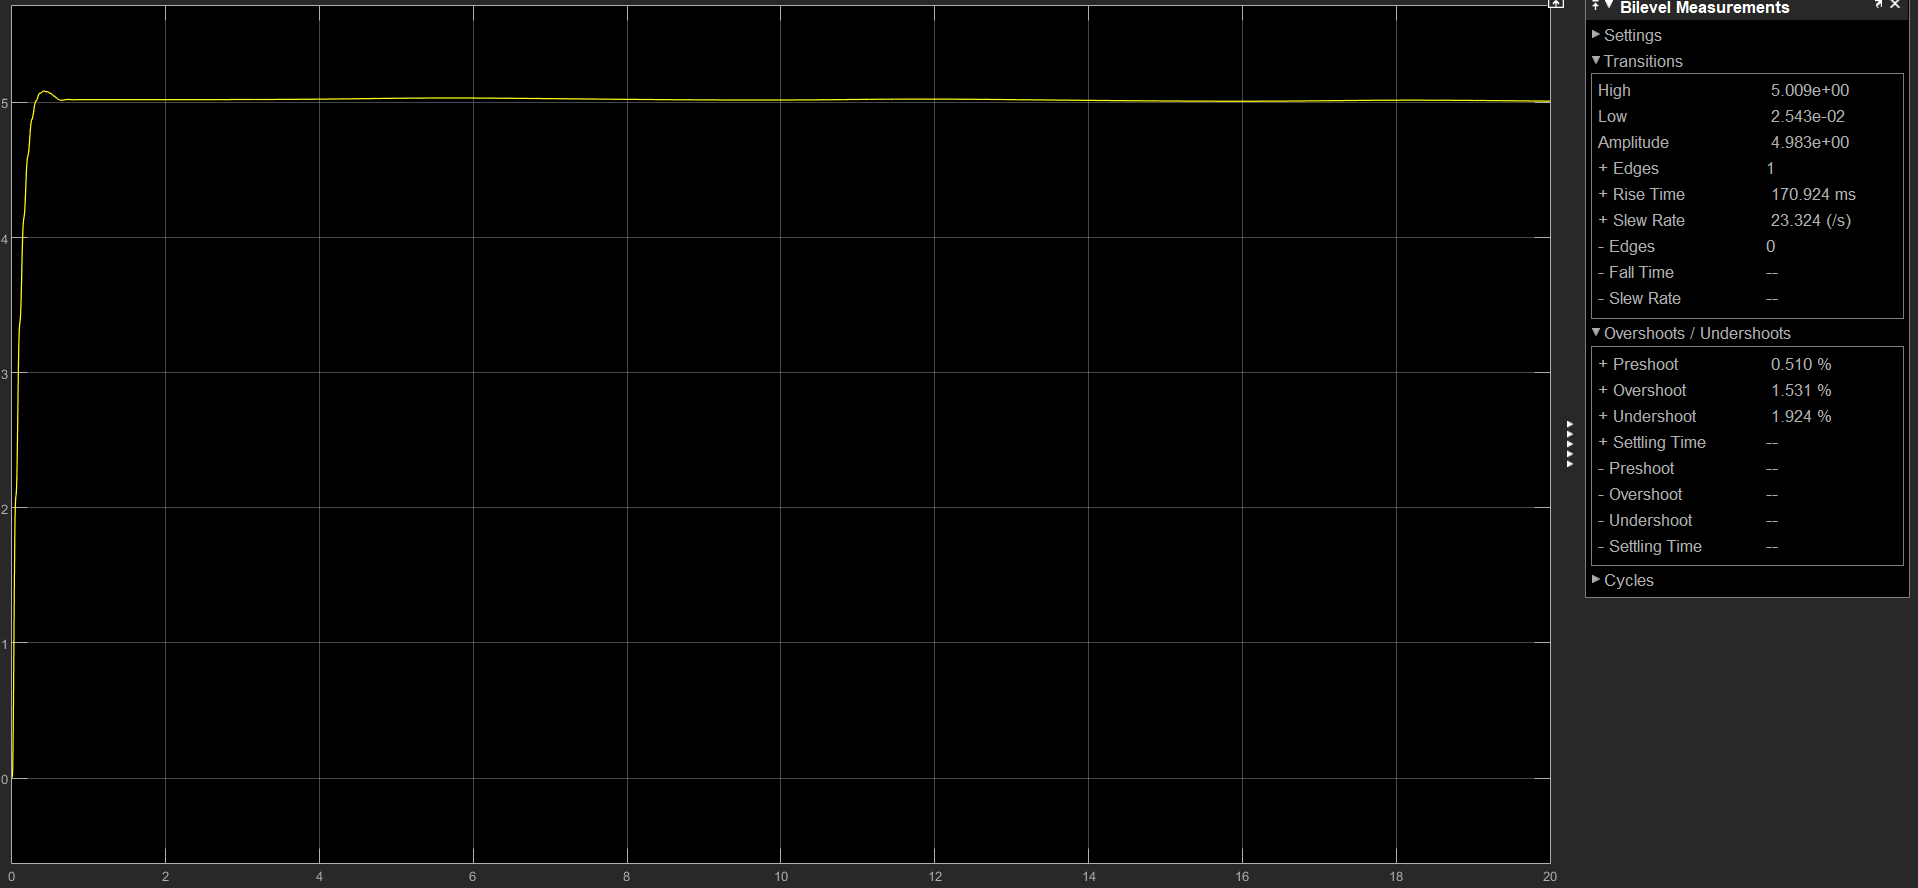
\includegraphics[width=1\linewidth]{../img/Q1_Constrained_TubeMPC_Response}
	\caption{تلاش کنترلی $Tube MPC$ مقید}
	\label{fig:q1constrainedtubempcresponse}
\end{figure}
\begin{figure}
	\centering
	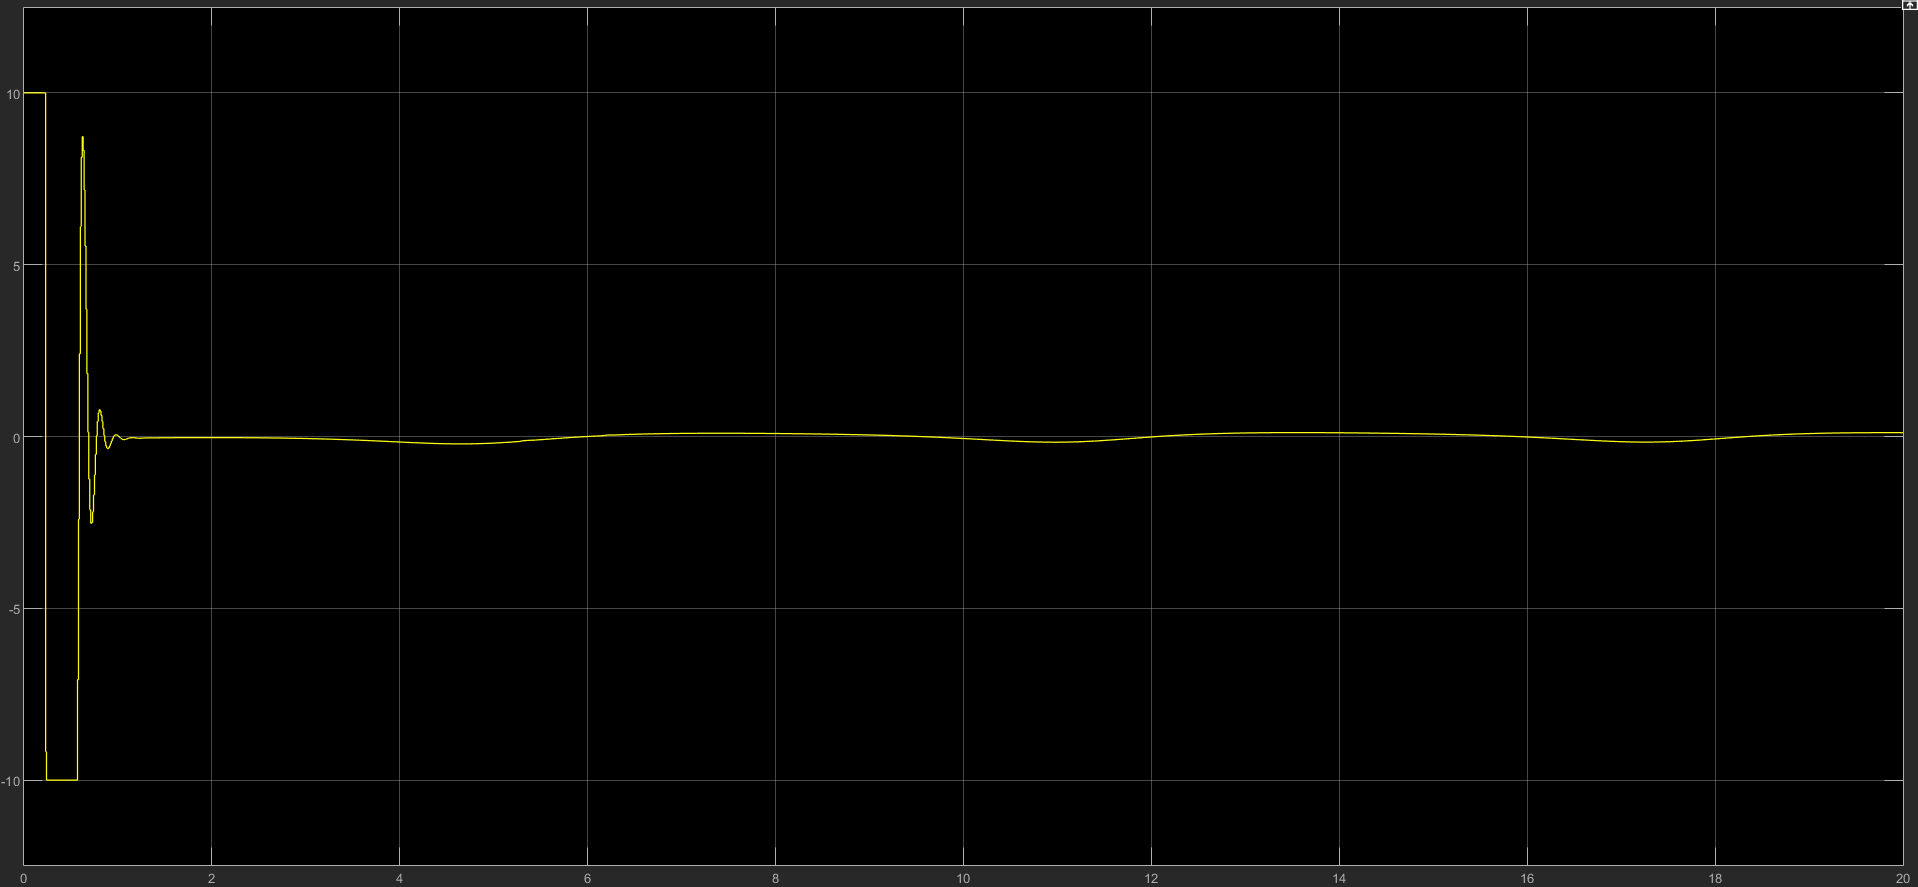
\includegraphics[width=1\linewidth]{../img/Q1_Constrained_TubeMPC_Ceffort}
	\caption{پاسخ $Tube MPC$ مقید}
	\label{fig:q1constrainedtubempcceffort}
\end{figure}

\section*{پاسخ سوال 2}
\subsection*{پاسخ بخش یکم}
در این سوال، با وجود معادلات حالت سیستم، می توان برای شبیه سازی آن را مستقیما به عنوان یک تابع در فضای سیمولینک تعریف کرد. برای این منظور، سیستمی به شکل زیر طراحی می شود.
\begin{figure}[H]
	\centering
	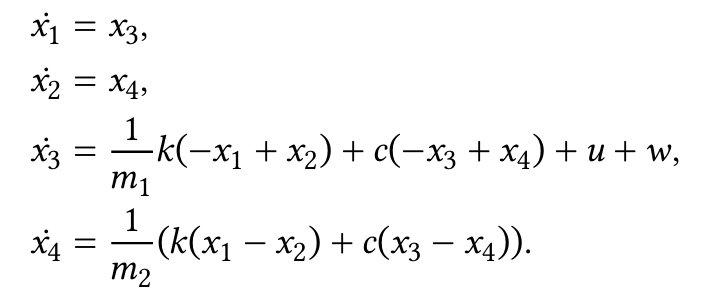
\includegraphics[width=0.7\linewidth]{../img/Q2_SS}
	\caption{معادلات حالت سیستم}
	\label{fig:q2ss}
\end{figure}
 در گام اول، سیستم مورد نظر در محیط سیمولینک تعریف شده و سپس پاسخ پله ی حلقه باز آن را بررسی می کنیم.
\begin{figure}[H]
	\centering
	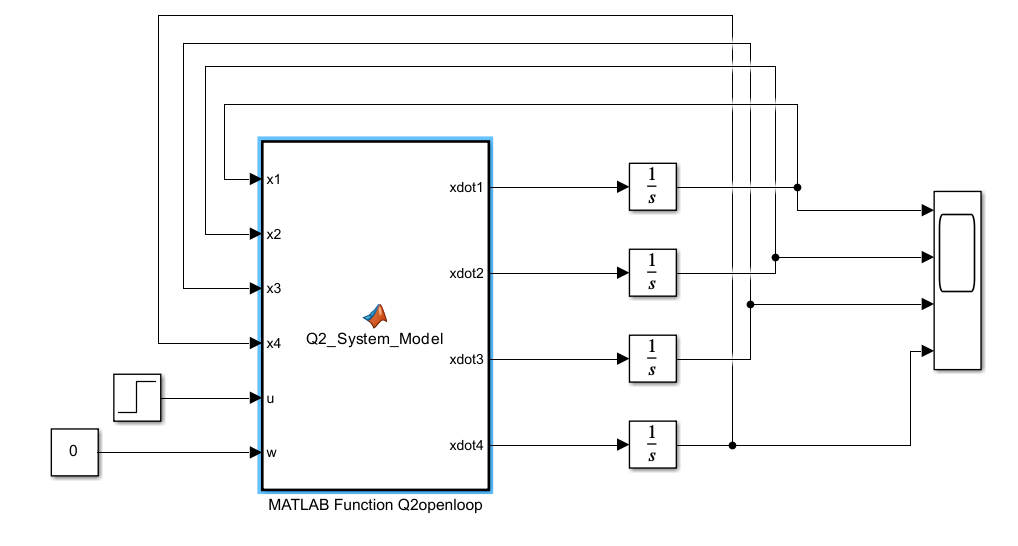
\includegraphics[width=1\linewidth]{../img/Q2_openloop_diagram}
	\caption{دیاگرام سیستم حلقه باز}
	\label{fig:q2openloopdiagram}
\end{figure}
\begin{figure}[H]
	\centering
	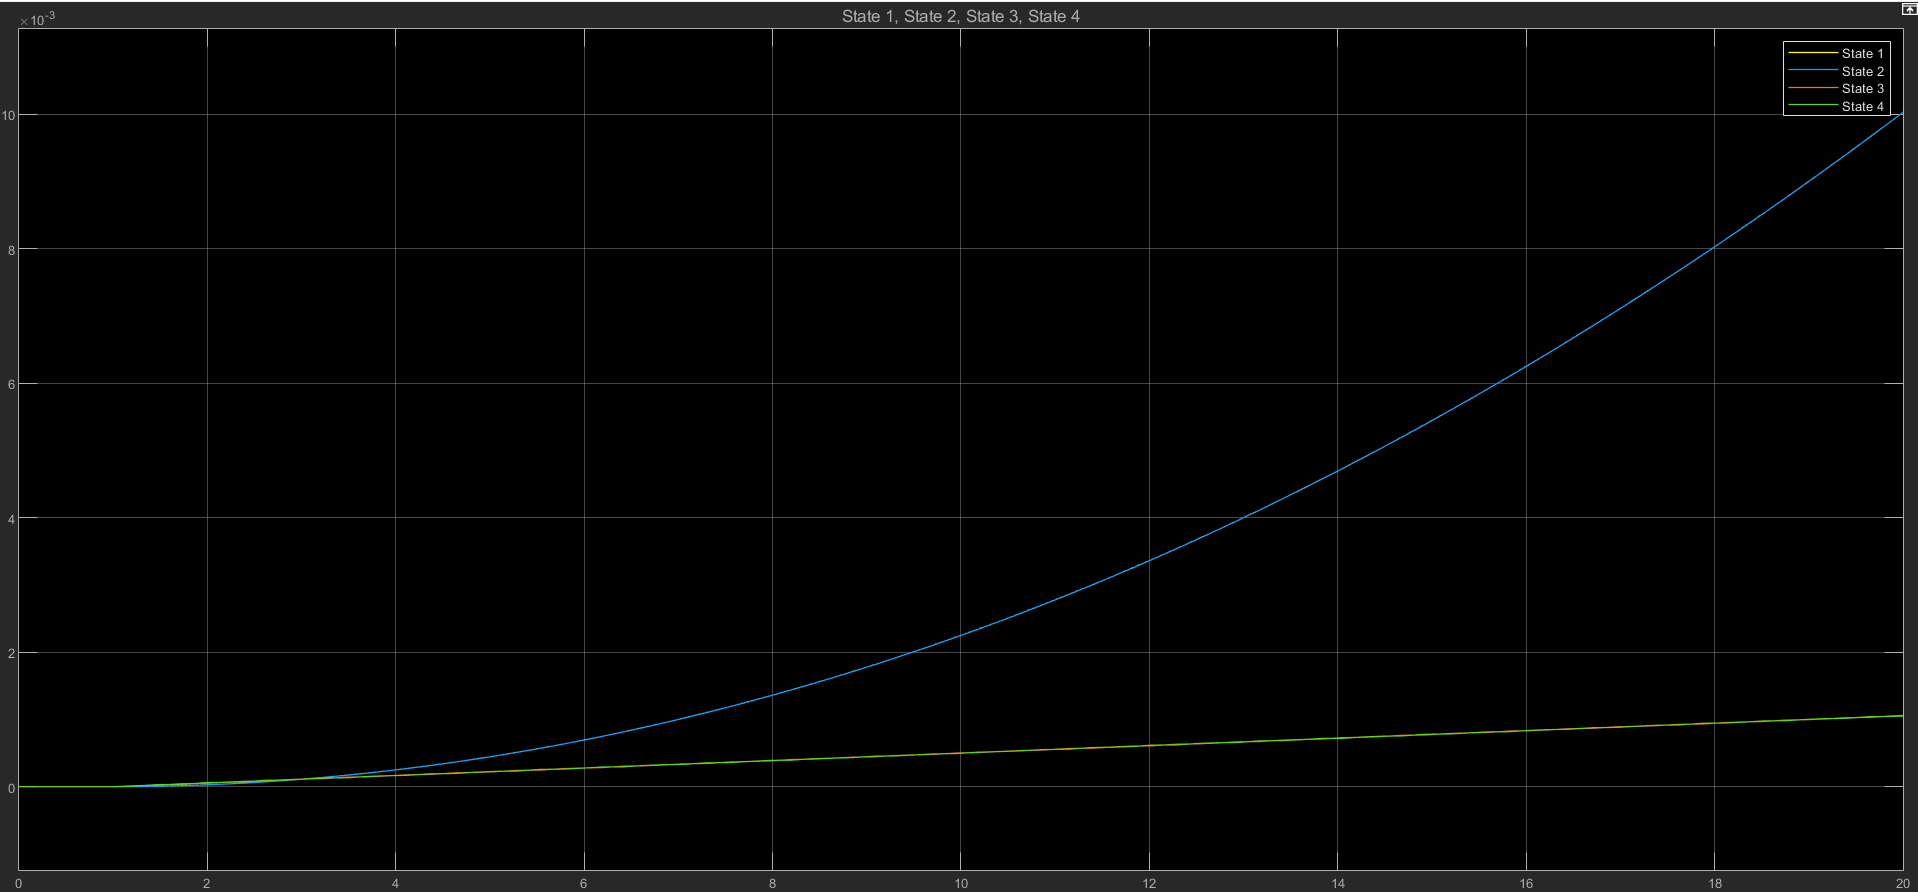
\includegraphics[width=1\linewidth]{../img/Q2_openloop_response}
	\caption{پاسخ پله ی حلقه باز}
	\label{fig:q2openloopresponse}
\end{figure}
مشاهده می شود که حالت های این سیستم به طور حلقه باز پایدار نیستند.
در ادامه با پیاده سازی یک کنترلر پیش بین خطی، سعی بر کنترل این سیستم خواهیم کرد. دیاگرام این سیستم به صورت زیر خواهد بود.
\begin{figure}[H]
	\centering
	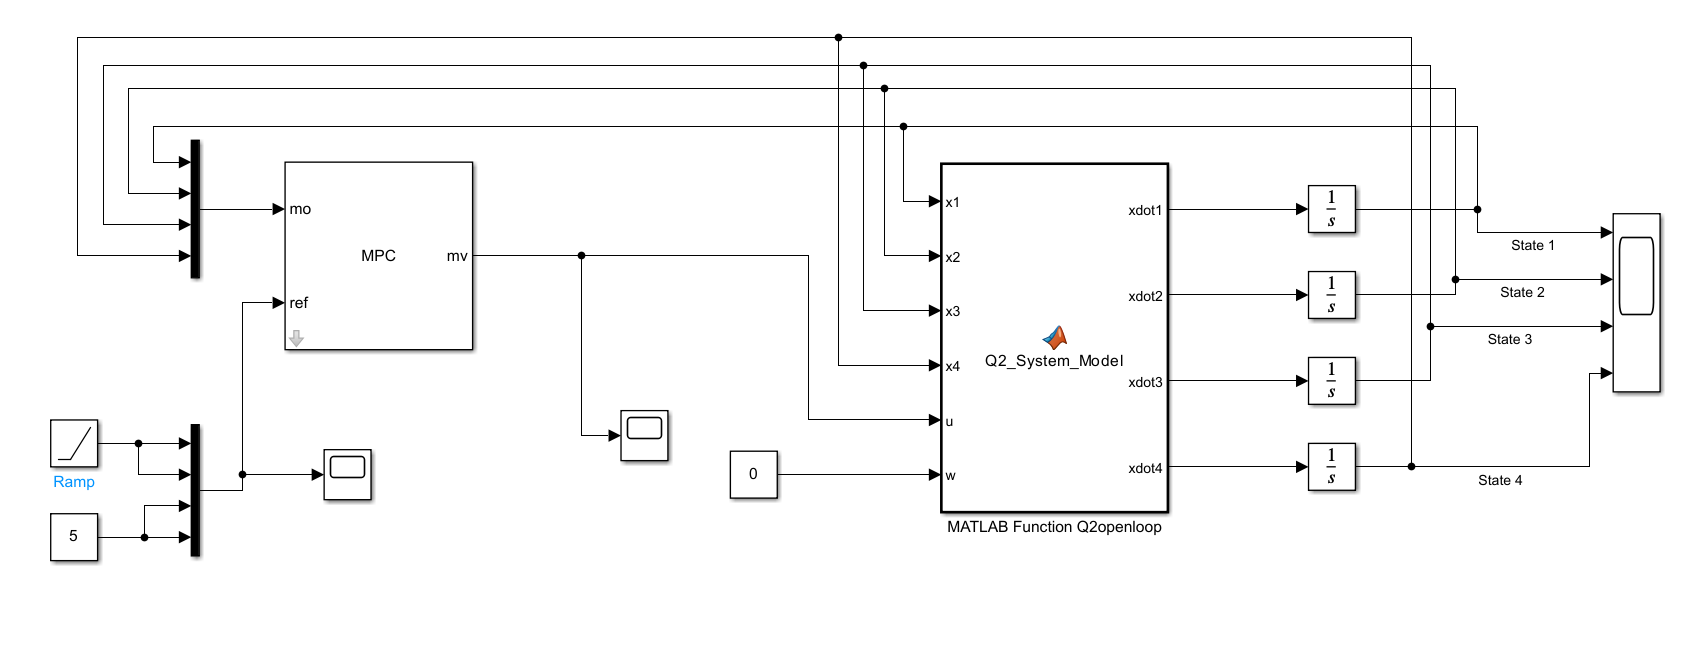
\includegraphics[width=1\linewidth]{../img/Q2_LMPC_diagram}
	\caption{دیاگرام سیستم}
	\label{fig:q2lmpcdiagram}
\end{figure}
برای تنظیم کنترلر پیش بین، از نرخ نمونه برداری $ 0.01 $ ثانیه، افق پیش بین 650 و افق کنترلی 100 استفاده شده است. پاسخ سیستم به ورودی های تعیین شده به صورت زیر به دست خواهد آمد

\begin{figure}[H]
	\centering
	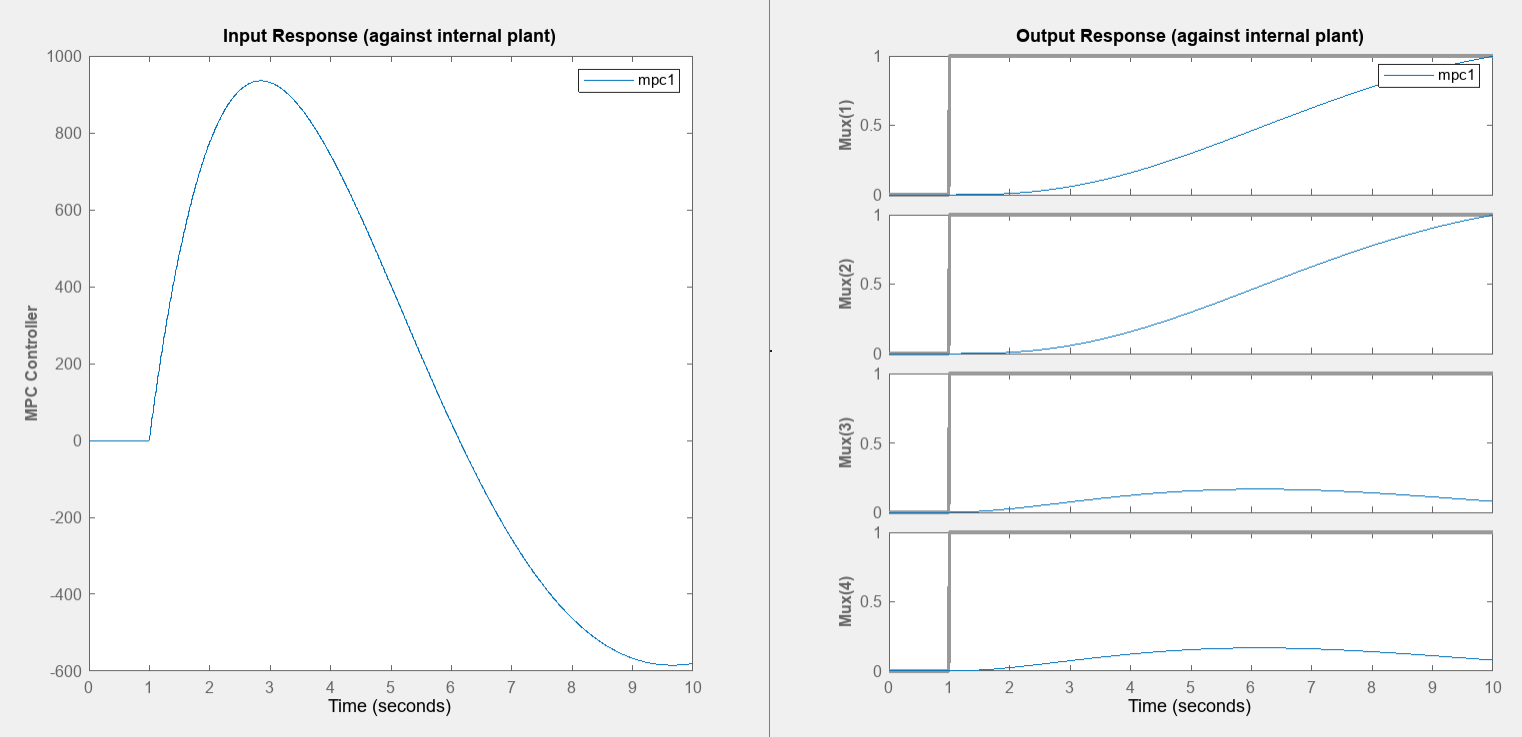
\includegraphics[width=1\linewidth]{../img/Q2_LMPC_ِDesign}
	\caption{پارامتر های کنترلر MPC}
	\label{fig:q2lmpcdesign}
\end{figure}

\begin{figure}[H]
	\centering
	\includegraphics[width=1\linewidth]{../img/Q2_LMPC_Response}
	\caption{پاسخ سیستم با کنترلر پیش بین خطی}
	\label{fig:q2lmpcresponse}
\end{figure}
با مشاهده ی پاسخ این سیستم متوجه می شویم که کنترلر حالت های اول و دوم را به خوبی کنترل کرده و خروجی، ورودی را دنبال می کند. اما برای حالت های سوم و چهارم، این اتفاق نمی افتد و مقدار خروجی با ورودی فاصله ی زیادی دارد.
همچنین، نمودار خروجی کنترلر به صورت زیر است:
\begin{figure}[H]
	\centering
	\includegraphics[width=1\linewidth]{../img/Q2_LMPC_ِCeffort}
	\caption{نمودار تلاش کنترلی}
	\label{fig:q2lmpcceffort}
\end{figure}
آنچنان که مشاهده می شود، مقدار فرمان کنترلی بسیار بزرگ است. برای جلوگیری از این کار و نرمالایز کردن کنترلر، می توان از بلوک های بهره برای افزایش مقادیر کنترلر استفاده کرد.
\subsection*{پاسخ بخش دوم}
\subsubsection{قسمت اول - قید نرم}
در این بخش، با اعمال یک قید نرم برای حالت چهارم، خروجی های سیستم را مجددا بررسی می کنیم.
\begin{figure}
	\centering
	\includegraphics[width=1\linewidth]{../img/Q2_LMPC_ِsoft_Response}
	\caption{پاسخ سیستم با قید نرم}
	\label{fig:q2lmpcsoftresponse}
\end{figure}
\begin{figure}[H]
	\centering
	\includegraphics[width=1\linewidth]{../img/Q2_LMPC_ِsoft_Ceffort}
	\caption{تلاش کنترلی}
	\label{fig:q2lmpcsoftceffort}
\end{figure}
\begin{figure}[H]
	\centering
	\includegraphics[width=1\linewidth]{../img/Q2_LMPC_ِsoft_setting}
	\caption{ورودی ها و خروجی ها}
	\label{fig:q2lmpcsoftsetting}
\end{figure}
\begin{figure}[H]
	\centering
	\includegraphics[width=0.7\linewidth]{../img/Q2_LMPC_ِsoft_setting1}
	\caption{تنظیمات قید ها}
	\label{fig:q2lmpcsoftsetting1}
\end{figure}
\subsubsection*{قسمت دوم - قید سخت}
حال در این بخش، با تغییر قید تعیین شده از حالت نرم به سخت، مجددا نتایج را بررسی می کنیم.
\begin{figure}[H]
	\centering
	\includegraphics[width=1\linewidth]{../img/Q2_LMPC_ِHard_Response}
	\caption{پاسخ سیستم}
	\label{fig:q2lmpchardresponse}
\end{figure}
\begin{figure}[H]
	\centering
	\includegraphics[width=0.7\linewidth]{"../img/Q2_LMPC_ِHard_Ceffort"}
	\caption{تلاش کنترلی}
	\label{fig:q2lmpchardceffort}
\end{figure}
\begin{figure}[H]
	\centering
	\includegraphics[width=0.7\linewidth]{"../img/Q2_LMPC_ِHard_Ceffort"}
	\caption{تنظیمات قید های سیستم}
	\label{fig:q2lmpchardsetting}
\end{figure}
با توجه به نتایح این قسمت و بخش پیشین، مشاهده می شود که تفات چندانی میان این دو روش وجود ندارد. علت این امر آن است که کنترلر در بخش ابتدایی توانسه با حداقل تلاش کنترلی، خروجی را کنترل کند و بنابراین نیازی به اعمال ورودی های بزرگ به سیستم نبوده. بنابراین، این سیستم در حالت عادی در حیطه ی قیدها قرار می گیرد و نیازی به تلاش مضاعف کنترلر و یا محدود کردن بازه های عملکردی آن نخواهد بود.
\subsection*{پاسخ بخش سوم}
در این بخش، با اعمال یک اغتشاش سینوسی به صورت زیر، عملکرد کنترلر را مورد بررسی قرار می دهیم. برای پیاده سازی این اغتشاش در محیط سیمولینک، از یک Function Block استفاده شده است.
\begin{figure}[H]
	\centering
	\includegraphics[width=0.7\linewidth]{../img/Q3_Disturbance}
	\caption{کد اغتشاش}
	\label{fig:q3disturbance}
\end{figure}
\begin{figure}[H]
	\centering
	\includegraphics[width=0.7\linewidth]{../img/Q3_Disturbance_plot}
	\caption{نمودار اغتشاش}
	\label{fig:q3disturbanceplot}
\end{figure}
\begin{figure}[H]
	\centering
	\includegraphics[width=1\linewidth]{../img/Q3_Diagram}
	\caption{دیاگرام سیستم با اغتشاش}
	\label{fig:q3diagram}
\end{figure}
به دلیل کوچک بودن مقدار اغتشاش ذکر شده در صورت سوال و قابل صرف نظر بودن از آن مقدار، در ادامه ی این آزمایش مقدار اغتشاش با دامنه ی 400 در نظر گرفته شده است تا یتوان نمایش بهتری از نمودار حاصل داشت.
در اینجا، خروچی سیستم را با این اغتشاش مشاهده می کنیم.
\begin{figure}[H]
	\centering
	\includegraphics[width=1\linewidth]{../img/Q3_High_disturbance}
	\caption{نمودار خروجی سیستم با اغتشاش}
	\label{fig:q3highdisturbance}
\end{figure}
\begin{figure}[H]
	\centering
	\includegraphics[width=1\linewidth]{../img/Q3_High_disturbance_Ceffort}
	\caption{نمودار تلاش کنترلر}
	\label{fig:q3highdisturbanceceffort}
\end{figure}
در این قسمت، با اضافه کردن یک بلوک کنترلر PID به سیستم، کنترلر $Tube MPC$ را تشکبل داده و نتایج سیستم را مجددا بررسی می کنیم.
ضرایب این کنترلر به دلیل حجم زیاد محاسبات، به وسیله تنظیم کننده متلب قابل تنظیم نبوده و به صورت دستی بر روی ضرایب زیر تنظیم شده است.
\begin{figure}[H]
	\centering
	\includegraphics[width=1\linewidth]{../img/Q3_High_disturbance_Tube_Response}
	\caption{نمودار خروجی های حالت سیستم}
	\label{fig:q3highdisturbancetuberesponse}
\end{figure}
\begin{figure}[H]
	\centering
	\includegraphics[width=1\linewidth]{../img/Q3_High_disturbance_Tube_Ceffort}
	\caption{نمودار تلاش کنترلر}
	\label{fig:q3highdisturbancetubeceffort}
\end{figure}
\begin{figure}[H]
	\centering
	\includegraphics[width=1\linewidth]{../img/Q3_High_disturbance_Tube_PID}
	\caption{ضرایب PID}
	\label{fig:q3highdisturbancetubepid}
\end{figure}
\subsection*{پاسخ بخش چهارم}
در این بخش، با اعمال مقادیری نایقینی مطابق آنچه که در صورت سوال ذکر شده است، به سیستم اعمال می کنیم. برای این کار، به مقادیر ورودی ها، مقادیر سینوسی متغیر با زمان با میزان مشخص شده اضافه می کنیم. سپس، مقادیر خروجی را با استفاده از کنترلر $Tube MPC$ و $Linear MPC$ طراحی شده کنترل می کنیم. 
سیستم کنترلی پیش بین خطی مطابق سیستم زیر مورد استفاده قرار گرفته است.
\begin{figure}[H]
	\centering
	\includegraphics[width=0.7\linewidth]{../img/Q4_Uncertainty_Responce_LinearMPC}
	\caption{نمودار خروجی با وجود نایقینی}
	\label{fig:q4uncertaintyresponcelinearmpc}
\end{figure}
\begin{figure}[H]
	\centering
	\includegraphics[width=0.7\linewidth]{../img/Q4_Uncertainty_Ceffort_LinearMPC}
	\caption{نمودار تلاش کنترلی با وجود نایقینی}
	\label{fig:q4uncertaintyceffortlinearmpc}
\end{figure}
در ادامه، با تغییر کنترلر به Tube MPC، مجددا سیگنال های کنترلی را بررسی می کنیم.
\begin{figure}[H]
	\centering
	\includegraphics[width=0.7\linewidth]{../img/Q4_Uncertainty_Responce_TubeMPC}
	\caption{نمودار خروجی سیستم با وجود نایقینی}
	\label{fig:q4uncertaintyresponcetubempc}
\end{figure}
\begin{figure}[H]
	\centering
	\includegraphics[width=0.7\linewidth]{../img/Q4_Uncertainty_Ceffort_TubeMPC}
	\caption{نمودار خروجی کنترلر بار وجود نایقینی}
	\label{fig:q4uncertaintycefforttubempc}
\end{figure}


		% فصل سوم: معرفی معماری POLO
%% !TeX root=../main.tex
\chapter{نتایج}
%\thispagestyle{empty} 
\label{chap:results}
\section{مقدمه} 
یکی از فصل‌های مهم  \پ  این فصل است که در آن به ارائهٔ داده‌ها، نتایج، تحلیل و تفسیر اولیهٔ آنها پرداخته می‌شود. در ارائهٔ نتایج تا حد امکان، ترکیبی از نمودارها و جداول استفاده شود، چراکه به کمک آن‌ها بهتر می‌توان نتایج کار را نمایش داد و نسبت به کار سایرین آن را متمایز کرد. با توجه به حجم و ماهیت تحقیق و با صلاحدید استاد راهنما، این فصل می‌تواند تحت عنوانی دیگر بیاید. در این فصل باید به سوالات تحقیق که در پیش‌تر در مقدمه و مروری بر ادبیات موضوع بیان شده است، بنابر یافته‌های محقق در روند انجام کار، پاسخ داده شود. اگر تحقیق دارای آزمون فرض باشد، پذیرش یا عدم پذیرش فرضیه‌ها در این فصل گزارش می‌شود. این فصل باید حدود 20 صفحه باشد.

\section{محتوا}
در این بخش به سوالات تحقیق، بر اساس داده‌ها و یافته‌های محقق، پاسخ داده می‌شود. داده‌ها با فرمت مناسبی ارائه می‌شوند؛ مدل (ها) اجرا شده و نتیجه آن مشخص می‌شود.

\section{اعتبارسنجی}
از طریق مقایسهٔ نتایج با نتایج کارهای دیگران، استفاده از روش‌های تحلیل پایائی
\lr{(reliability)}
و اعتبار
\lr{(validity)}،
نظرگیری از خبرگان
\lr{(expert judgment or feedback)}
و یا
\lr{triangulation}
انجام می‌شود.
		% فصل چهارم: نتایج
%% !TeX root=../main.tex
\chapter{بحث و نتیجه‌گیری}
%\thispagestyle{empty} 


این گزارش به‌صورت جامع به بررسی طراحی و ساخت موتورهای مسطح مبتنی بر شناوری مغناطیسی (MLPM) پرداخته و جنبه‌های مختلف این سیستم‌ها شامل معماری، طراحی آهنرباهای دائمی، سیستم‌های کنترلی و روش‌های مدل‌سازی را مورد تحلیل قرار داده است. هدف اصلی این تحلیل‌ها، شناسایی بهترین روش‌ها و ارائه راهکارهایی برای بهبود عملکرد این دستگاه‌ها بر اساس پژوهش‌های پیشین بوده است.
در معماری دستگاه، بررسی‌ها نشان داد که استفاده از سیم‌پیچ‌های متحرک و آهنرباهای ثابت به دلیل محدودیت‌های ذاتی مانند مشکلات مرتبط با اتصالات الکتریکی و خنک‌کاری سیم‌پیچ‌ها، راهکاری با کارایی کمتر محسوب می‌شود. در مقابل، استفاده از سیم‌پیچ‌های ثابت و آهنرباهای دائمی متحرک، به دلیل حذف محدودیت‌های فوق و بهبود عملکرد حرکتی بخش متحرک، به‌عنوان معماری بهینه و مناسب‌تر برای کاربردهای MLPM معرفی شد.
در طراحی آهنرباهای دائمی، مقایسه بین آهنرباهای دیسکی و آرایه‌های هالباخ نشان داد که آرایه‌های هالباخ به‌ویژه در چینش‌های یک‌بعدی و دوبعدی، عملکرد بهتری از نظر تقویت میدان مغناطیسی دارند. این آرایه‌ها، از طریق خنثی کردن میدان در یک سمت و تقویت آن در سمت دیگر، قادر به تولید میدان مغناطیسی قوی‌تری هستند که امکان کنترل دقیق‌تر نیروها و جابه‌جایی‌ها را فراهم می‌آورد. آهنرباهای دیسکی هرچند از نظر طراحی ساده‌تر هستند، اما به دلیل ناپایداری و غیر یکنواختی میدان مغناطیسی، کارایی کمتری در سیستم‌های MLPM دارند. آرایه‌های دوبعدی هالباخ، هرچند مزیت‌های بسیاری در تقویت میدان مغناطیسی دارند، با چالش‌هایی همچون ایجاد نوسانات بیشتر در میدان همراه هستند که باید با استفاده از طراحی دقیق‌تر مدیریت شود.
در حوزه کنترلرها، کنترلرهای کلاسیک نظیر PID به دلیل سادگی و کارایی اثبات‌شده، همچنان به‌عنوان گزینه‌ای مناسب برای سیستم‌های MLPM مطرح هستند. با این حال، نتایج پژوهش‌ها نشان می‌دهد که در صورتی که اطلاعات دینامیکی سیستم در دسترس باشد، کنترلرهای مبتنی بر مدل پیش‌بینی (MPC) و یا کنترلرهای مبتنی بر هوش مصنوعی همچون GRU، به دلیل توانایی پیش‌بینی رفتار سیستم و اعمال کنترل دقیق‌تر، از عملکرد بهتری برخوردارند. این روش‌های پیشرفته می‌توانند پایداری سیستم را افزایش داده و خطاهای ناشی از کنترل را کاهش دهند، به‌ویژه در کاربردهایی که نیاز به دقت بالا دارند.

		% فصل پنجم: بحث و نتیجه‌گیری

% مراجع
% اگر از استیل‌های natbib استفاده می‌کنید باید دو خط را در فایل commands.tex تغییر دهید.
%\pagestyle{empty}
%\newpage
%{
%\small
%\onehalfspacing
%\bibliographystyle{unsrt-fa} % or plainnat-fa for author-date
%\bibliography{./tex/MyReferences}
%}

\pagestyle{fancy}

%\appendix
% فصلهای پس از این قسمت به عنوان ضمیمه خواهند آمد.

% دستورات لازم برای تبدیل «فصل آ» به «پیوست آ» در فهرست مطالب

%\addtocontents{toc}{
%\protect\renewcommand\protect\cftchappresnum{\appendixname~}%
%\protect\setlength{\cftchapnumwidth}{\mylenapp}}
    
% دستورات لازم برای شماره‌گذاری صفحات پیوست‌ها بشکل آ-۱ (فعلا با glossaries سازگار نیست)
%\let\Chapter\chapter
%\pretocmd{\chapter}{
%\clearpage
%\pagenumbering{arabic}
%\renewcommand*{\thepage}{\rl{\thechapter-\arabic{page}}}}{}{}
%%%%%%%%%%%%%%%%%%%%%%%%%%%%%%%%%%%%%        

%% !TeX root=../main.tex

\chapter{آشنایی سریع با برخی دستورات لاتک}
\label{app:latexIntro}
%\thispagestyle{empty}
در این فصل ویژگی‌های مهم و پرکاربرد زی‌پرشین و لاتک معرفی می‌شود. برای راهنمایی بیشتر و به‌کاربردن ویژگی‌های پیشرفته‌تر به راهنمای زی‌پرشین و راهنمای لاتک مراجعه کنید. برای آگاهی از دستورات لاتک که این خروجی را تولید کرده‌اند فایل \lr{appendix1.tex} را ملاحظه فرمایید.
\footnote{بیشتر مطالب این بخش از مثال 
	\lr{xepersian\_example.tex}
	گرفته شده‌اند که توسط آقای امیرمسعود پورموسی آماده شده است.}

\section{بندها و زیرنویس‌ها}
هر جایی از نوشتهٔ خود، اگر می‌خواهید به سر سطر بروید و یک بند (پاراگراف) تازه را آغاز کنید، باید یک خط را خالی بگذارید%
\footnote{یعنی دوبار باید کلید \lr{Enter} را بزنید.}
مانند این:

حالا که یک بند تازه آغاز شده است، یک زیرنویس انگلیسی%
\LTRfootnote{English Footnote!}
هم می‌نویسیم!
\section{فرمول‌های ریاضی}
\label{formula}

اینجا هم یک فرمول می‌آوریم که شماره دارد:
\begin{equation}\label{eq:yek}
	A=\frac{c}{d}+\frac{q^2}{\sin(\omega t)+\Omega_{12}}
\end{equation}
در لاتک می‌توان به کمک فرمان 
\lr{\textbackslash label\{\}}
به هر فرمول یک نام نسبت داد. در فرمول بالا نام \lr{eq:yek} را برایش گذاشته‌ایم (پروندهٔ \lr{tex} همراه با این مثال را ببینید). این نام ما را قادر می‌کند که بعداً بتوانیم با فرمان
\lr{\textbackslash ref\{eq:yek\}}
به آن فرمول با شماره ارجاع دهیم. یعنی بنویسیم فرمول \ref{eq:yek}. 
لاتک خودش شمارهٔ این فرمول‌ها را مدیریت می‌کند.\footnote{یعنی اگر بعداً فرمولی قبل از این فرمول بنویسیم، خودبه‌خود شمارهٔ این فرمول و شمارهٔ ارجاع‌ها به این فرمول یکی زیاد می‌شود. دیگر نگران شماره‌گذاری فرمول‌های خود نباشید!} این هم یک فرمول که شماره ندارد:
$$A=|\vec{a}\times \vec{b}| + \sum_{n=0}^\infty C_{ij}$$

این هم عبارتی ریاضی مانند 
$\sqrt{a^2+b^2}$
که بین متن می‌آید.
\subsection{یک زیربخش}
\label{zirbakhsh}

این زیربخش \ref{zirbakhsh} است؛ یعنی یک بخش درون بخش \ref{formula} است.
\subsubsection{یک زیرزیربخش}
این هم یک زیرزیربخش است. در لاتک می‌توانید بخش‌های تودرتو در نوشته‌تان تعریف کنید تا ساختار منطقی نوشته را به خوبی نشان دهید. می‌توانید به این بخش‌ها هم با شماره ارجاع دهید، مثلاً بخش فرمول‌های ریاضی شماره‌اش \ref{formula} است.
\section{نوشته‌های فارسی و انگلیسی مخلوط}
نوشتن یک کلمهٔ انگلیسی بین متن فارسی بدیهی است، مانند Example در این جمله.\footnote{هرچند بهتر است باز هم آن کلمه را مانند \lr{Example} در این جمله بنویسید.}
نوشتن یک عبارت چندکلمه‌ای مانند
\lr{More than one word} کمی پیچیده‌تر است.

اگر ناگهان تصمیم بگیرید که یک بند کاملاً انگلیسی را بنویسید، باید:
\begin{latin}
	This is an English paragraph from left to right. You can write as much as you want in it.
\end{latin}
\section{افزودن تصویر به نوشته}
پروندهٔ تصویر دلخواه خود را در کنار پروندهٔ \lr{tex} قرار دهید. سپس به روش زیر تصویر را در نوشتهٔ خود بیاورید:
\begin{latin}
	\begin{verbatim}
		\includegraphics{YourImageFileName}
	\end{verbatim}
\end{latin}
به تصویرها هم مانند فرمول‌ها و بخش‌ها می‌توان با شماره ارجاع داد. مثلاً تصویر \ref{fig:shir} یک شیر علاقه‌مند به لاتک را در حال دویدن نشان می‌دهد. برای جزئیات بیشتر دربارهٔ روش گذاشتن تصویرها در نوشته باید راهنماهای لاتک را بخوانید.
\begin{figure}[ht]
	\centerline{\includegraphics[width=5cm]{lion}}
	\caption{در این تصویر یک شیر علاقه‌مند به لاتک را در حال دویدن می‌بینید.}
	\label{fig:shir}
\end{figure}

به تصویرها هم مانند فرمول‌ها و بخش‌ها می‌توان با شماره ارجاع داد. مثلاً تصویر بالا شماره‌اش \ref{fig:shir} است. برای جزئیات بیشتر دربارهٔ روش گذاشتن تصویرها در نوشته باید راهنماهای لاتک را بخوانید.

\section{محیط‌های شمارش و نکات}
برای فهرست‌کردن چندمورد، اگر ترتیب برایمان مهم نباشد:
\begin{itemize}
	\item مورد یکم
	\item مورد دوم
	\item مورد سوم
\end{itemize}
و اگر ترتیب برایمان مهم باشد:
\begin{enumerate}
	\item مورد یکم
	\item مورد دوم
	\item مورد سوم
\end{enumerate}
می‌توان موردهای تودرتو داشت:
\begin{enumerate}
	\item مورد ۱
	\item مورد ۲
	\begin{enumerate}
		\item مورد ۱ از ۲
		\item مورد ۲ از ۲
		\item مورد ۳ از ۲
	\end{enumerate}
	\item مورد ۳
\end{enumerate}
شماره‌گذاری این موردها را هم لاتک انجام می‌دهد.

\section{تعریف و قضیه}\label{app:index}
برای ذکر تعریف، قضیه و مثال مثالهای ذیل را ببینید.
\begin{definition}
	مجموعه همه ارزیابی‌های  (پیوسته)  روی $(X,\tau)$، دامنه توانی احتمالی
	\index{دامنه توانی احتمالی}
	$ X $
	نامیده می‌شود.
\end{definition}
\begin{theorem}[باناخ-آلااغلو]
	\index{قضیه باناخ-آلااغلو}
	اگر $ V $ یک همسایگی $ 0 $ در فضای برداری 
	\index{فضای!برداری}
	توپولوژیکی $ X $ باشد و 
	\begin{equation}\label{eq1}
		K=\left\lbrace \Lambda \in X^{*}:|\Lambda x|\leqslant 1 ; \ \forall x\in V\right\rbrace,
	\end{equation}
	آنگاه $ K $،  ضعیف*-فشرده است که در آن، $ X^{*} $ دوگان
	\index{فضای!دوگان}
	فضای برداری توپولوژیکی $ X $ است به ‌طوری که عناصر آن،  تابعی‌های 
	خطی پیوسته
	\index{تابعی خطی پیوسته}
	روی $X$ هستند.
\end{theorem}
تساوی \eqref{eq1} یکی از مهم‌ترین تساوی‌ها در آنالیز تابعی است که در ادامه، به وفور از آن استفاده می‌شود.
\begin{example}
	برای هر فضای مرتب، گردایه 
	$$U:=\left\lbrace U\in O: U=\uparrow U\right\rbrace $$
	از مجموعه‌های بالایی باز، یک توپولوژی تعریف می‌کند که از توپولوژی اصلی، درشت‌تر  است.
\end{example}
حال تساوی 
\begin{equation}\label{eq2}
	\sum_{n=1}^{+\infty} 3^{n}x+7x=\int_{1}^{n}8nx+\exp{(2nx)}
\end{equation}
را در نظر بگیرید. با مقایسه تساوی \eqref{eq2} با تساوی \eqref{eq1} می‌توان نتیجه گرفت که ...


\section{چگونگی نوشتن و ارجاع به مراجع}
\label{Sec:Ref}


در لاتک به راحتی می‌توان مراجع خود را نوشت و به آنها ارجاع داد. به عنوان مثال برای معرفی کتاب گنزالس \cite{Gonzalez02book} به عنوان یک مرجع می‌توان آنرا به صورت زیر معرفی نمود:

\singlespacing
\begin{LTR}
	\begin{verbatim}
		\bibitem{Gonzalez02book}
		Gonzalez, R.C., and Woods, R.E. {\em Digital Image Processing}, 3rd ed..
		Prentice-Hall, Inc., Upper Saddle River, NJ, USA, 2006.
	\end{verbatim}
\end{LTR}
\doublespacing

در دستورات فوق \lr{Gonzalez02book}  برچسبی است که به این مرجع داده شده است و با استفاده از دستور 
\verb!\cite{Gonzalez02book}!
می‌توان به آن ارجاع داد؛ بدون این که شماره‌اش را در فهرست مراجع‌مان بدانیم.

اگر این اولین مرجع ما باشد در قسمت مراجع به صورت زیر خواهد آمد:\\
\includegraphics[width=\textwidth]{gonzalez.png}

این شیوهٔ تعریف مراجع بسیار ابتدایی است و اگر فرمت مراجع، ترتیب یا تعداد آنها را خواسته باشید تغییر دهید، به عنوان مثال ابتدا حرف اول نام نویسنده بیاید و سپس نام خانوادگی، باید همه کارها را به صورت دستی انجام دهید!
چون در یک \پ یا مقاله باید کنترل کاملی بر مراجع خود داشته باشید و به راحتی بتوانید قالب مراجع را عوض کنید، بنابراین می‌بایست از \lr{Bib\TeX} استفاده کنید که درپیوست  \ref{app:refMan} به  آن پرداخته خواهد شد.
		% پیوست اول: آشنایی مقدماتی با لاتک
%% !TeX root=../main.tex

\chapter{‌جدول، نمودار و الگوریتم در لاتک}
\label{app:latex:more}
%\thispagestyle{empty}

در این بخش نمونه مثالهایی از جدول، شکل، نمودار، الگوریتم و معادلات ریاضی را در لاتک خواهیم دید.
دقت کنید که در پایان‌نامه‌ها و مقالات، باید قاعدهٔ «ارجاع به جلو%
\LTRfootnote{Forward Referencing}»
رعایت شود؛ یعنی ابتدا در متن به شمارهٔ شکل، جدول یا معادله اشاره شود و بعد از آن (زیر آن) خود شکل، جدول یا معادله رسم شود. (توضیحات بیشتر در قسمت
\ref{sec:floatObjs}).

\section{جدول}
دستور اصلی برای رسم جدول در لاتک 
\verb|tabular|
می‌باشد که جدول
\eqref{tab:motionModels}
با استفاده از آن کشیده شده است؛ در
\verb|tabular|
عرض جدول برابر با مجموع عرض ستون‌ها و حداکثر مساوی عرض متن است.
\begin{table}[ht]
\caption{مدلهای تبدیل.}
\label{tab:motionModels}
\centering
\onehalfspacing
\begin{tabular}{|r|c|l|r|}
	\hline نام مدل & درجه آزادی & تبدیل مختصات & توضیح \\ 
	\hline انتقالی & ۲ & $\begin{aligned} x'=x+t_x \\ y'=y+t_y \end{aligned}$  &  انتقال دوبعدی\\ 
	\hline اقلیدسی & ۳ & $\begin{aligned} x'=x\cos\theta - y\sin\theta+t_x \\ y'=x\sin\theta+y\cos\theta+t_y \end{aligned}$  &  انتقالی+دوران \\ 
	\hline 
\end{tabular} 
\end{table}

برای اینکه عرض جدول قابل کنترل باشد، باید از دستورات
\verb|tabularx|،
\verb|tabulary| یا
\verb|tabu|
استفاده کرد که راهنمای آنها در اینترنت وجود دارد.
مثلاً جدول
\ref{tab:motionModelsCont}
با
\verb|tabularx|
رسم شده که عرض جدول در آن ثابت بوده و ستون‌های از نوع
\verb|X|
عرض خالی جدول را پر می‌کنند.
\begin{table}[ht]
	\caption{مدلهای تبدیل دیگر.}
	\label{tab:motionModelsCont}
	\centering
	\onehalfspacing
	\begin{tabularx}{\textwidth}{|r|c|l|X|}
		\hline نام مدل & درجه آزادی & تبدیل مختصات & توضیح \\ 
		\hline مشابهت & ۴ & $\begin{aligned} x'=sx\cos\theta - sy\sin\theta+t_x \\ y'=sx\sin\theta+sy\cos\theta+t_y  \end{aligned}$  & اقلیدسی+تغییرمقیاس \\ 		
		\hline آفین & ۶ & $\begin{aligned} x'=a_{11}x+a_{12}y+t_x \\ y'=a_{21}x+a_{22}y+t_y \end{aligned}$  & مشابهت+اریب‌شدگی \\
		\hline
	\end{tabularx}
\end{table}

\section{معادلات ریاضی و ماتریس‌ها}
تقریباً هر آنچه دانشجویان برای نوشتن فرمول‌های ریاضی لازم دارند، در کتاب 
\lr{mathmode}
آمده است. کافیست در خط فرمان، دستور زیر را وارد کنید:
\begin{latin}
	\texttt{texdoc mathmode}
\end{latin}
متن زیر شامل انواعی از اشیاء ریاضی است که با ملاحظه کدش می‌توانید با دستورات آن آشنا شوید.\\
شناخته‌شده‌ترین روش تخمین ماتریس هوموگرافی الگوریتم تبدیل خطی مستقیم (\lr{DLT\LTRfootnote{Direct Linear Transform}}) است.  فرض کنید چهار زوج نقطهٔ متناظر در دو تصویر در دست هستند،  $\mathbf{x}_i\leftrightarrow\mathbf{x}'_i$   و تبدیل با رابطهٔ
  $\mathbf{x}'_i = H\mathbf{x}_i$
  نشان داده می‌شود که در آن:
\[\mathbf{x}'_i=(x'_i,y'_i,w'_i)^\top  \]
و
\[ H=\left[
\begin{array}{ccc}
h_1 & h_2 & h_3 \\ 
h_4 & h_5 & h_6 \\ 
h_7 & h_8 & h_9
\end{array} 
\right]\]
رابطه زیر را برای الگوریتم  \eqref{alg:DLT} لازم داریم.
\begin{equation}
\label{eq:DLT_Ah}
\left[
\begin{array}{ccc}
	0^\top & -w'_i\mathbf{x}_i^\top & y'_i\mathbf{x}_i^\top \\ 
	w'_i\mathbf{x}_i & 0^\top & -x'_i\mathbf{x}_i^\top \\ 
	- y'_i\mathbf{x}_i^\top & x'_i\mathbf{x}_i^\top & 0^\top
\end{array} 
\right]
\left(
\begin{array}{c}
	\mathbf{h}^1 \\ 
	\mathbf{h}^2 \\ 
	\mathbf{h}^3
\end{array} 
\right)=0
\end{equation}

\section{الگوریتم}

\subsection{الگوریتم ساده با دستورهای فارسی}
با مفروضات فوق، الگوریتم \lr{DLT} به صورت نشان داده شده در الگوریتم \eqref{alg:DLT}  خواهد بود.
\begin{algorithm}[ht]
\onehalfspacing
\caption{الگوریتم \lr{DLT} برای تخمین ماتریس هوموگرافی.} \label{alg:DLT}
\begin{algorithmic}[1]
\REQUIRE $n\geq4$ زوج نقطهٔ متناظر در دو تصویر 
${\mathbf{x}_i\leftrightarrow\mathbf{x}'_i}$،\\
\ENSURE ماتریس هوموگرافی $H$ به نحوی‌که: 
$\mathbf{x}'_i = H \mathbf{x}_i$.
  \STATE برای هر زوج نقطهٔ متناظر
$\mathbf{x}_i\leftrightarrow\mathbf{x}'_i$ 
ماتریس $\mathbf{A}_i$ را با استفاده از رابطهٔ \ref{eq:DLT_Ah} محاسبه کنید.
  \STATE ماتریس‌های ۹ ستونی  $\mathbf{A}_i$ را در قالب یک ماتریس $\mathbf{A}$ ۹ ستونی ترکیب کنید. 
  \STATE تجزیهٔ مقادیر منفرد \lr{(SVD)}  ماتریس $\mathbf{A}$ را بدست آورید. بردار واحد متناظر با کمترین مقدار منفرد جواب $\mathbf{h}$ خواهد بود.
  \STATE  ماتریس هوموگرافی $H$ با تغییر شکل $\mathbf{h}$ حاصل خواهد شد.
\end{algorithmic}
\end{algorithm}

\subsection{الگوریتم پیچیده و تودرتو با دستورهای فارسی}
الگوریتم \ref{alg:simulation-random}، یک الگوریتم ترکیبی و تودرتو است که با کمک دستورهای بستهٔ \lr{algorithmic} نوشته شده است.

\begin{algorithm}[p]
    \onehalfspacing
    \caption{الگوریتم اجرای برنامهٔ شبیه‌سازی}
    \label{alg:simulation-random}
    \begin{algorithmic}[1]
        \REQUIRE زمان $t_{max}$ به عنوان زمان لازم برای انجام شبیه سازی،\\
        \REQUIRE  گراف شبکه برای شبیه سازی،
        \ENSURE جدول تغییرات گراف از لحظهٔ ۰ تا t.
        \FOR {تمام لحظات در بازهٔ ۰ تا $t_{max}$}
            \FOR {تمام پیوند‌ها}
                \STATE محاسبهٔ ضریب و نرخ انتقال پیوند
                \STATE محاسبهٔ کیفیت و نرخ یادگیری
            \ENDFOR
            \FOR {تمام گره‌ها}
                \STATE محاسبهٔ نرخ انتقال گره
                \STATE محاسبهٔ وضعیت جدید
            \ENDFOR
            \IF {تغییرات از مقدار $\delta$ کمتر است}
                \STATE شکستن حلقه
                \COMMENT{این شرط برای پایان قبل از رسیدن به محدودیت زمانی است، اگر تغییرات کمتر از $\delta$ باشد}
            \ELSIF {زمان اجرای برنامه بیش از حد طول کشیده \AND $t>100$}
                \STATE شکستن حلقه
            \ENDIF
        \ENDFOR
        \PRINT {زمان اجرای برنامه}
        \RETURN {ماتریس تغییرات زمانی}
    \end{algorithmic}
\end{algorithm}

\subsection{الگوریتم با دستورهای لاتین}
الگوریتم \ref{alg:RANSAC} یک الگوریتم با دستورهای لاتین است.

\begin{algorithm}[ht]
\onehalfspacing
\caption{الگوریتم \lr{RANSAC} برای تخمین ماتریس هوموگرافی.} \label{alg:RANSAC}
\begin{latin}
\begin{algorithmic}[1]
\REQUIRE $n\geq4$ putative correspondences, number of estimations, $N$, distance threshold $T_{dist}$.\\
\ENSURE Set of inliers and Homography matrix $H$.
\FOR{$k = 1$ to $N$}
  \STATE Randomly choose 4 correspondence,
  \STATE Check whether these points are colinear, if so, redo the above step
  \STATE Compute the homography $H_{curr}$ by DLT algorithm from the 4 points pairs,
  \STATE $\ldots$ % الگوریتم کامل نیست
  \ENDFOR
  \STATE Refinement: re-estimate H from all the inliers using the DLT algorithm.
\end{algorithmic}
\end{latin}
\end{algorithm}

\section{کد}
درج کد به زبان‌های مختلف به سادگی امکان‌پذیر است. برنامه
\ref{code:matlabEx}
یک قطعه کد
\lr{MATLAB}
را نشان می‌دهد.
\begin{figure}[ht]
	\begin{LTR}
        \singlespacing
		\lstinputlisting[language=MATLAB, caption={نمونه کد \lr{MATLAB}}, label={code:matlabEx}]{MatlabExample.m}
        % \doublespacing
	\end{LTR}
\end{figure}

\section{تصویر}
نمونهٔ یک تصویر را در فصل قبل دیدیم. دو تصویر شیر کنار هم را نیز در شکل
\ref{fig:twoLion}
مشاهده می‌کنید.
\begin{figure}[ht]
\centering 
\subfloat[شیر ۱]{ \label{fig:twolion:one}
\includegraphics[width=0.3\textwidth]{lion}}
%\hspace{2mm}
\subfloat[شیر ۲]{ \label{fig:twolion:two}
\includegraphics[width=0.3\textwidth]{lion}}%
\caption{دو شیر}
\label{fig:twoLion} %% label for entire figure
\end{figure}

\section{نمودار}
لاتک بسته‌هایی با قابلیت‌های زیاد برای رسم انواع مختلف نمودارها دارد. مانند بسته‌های \lr{Tikz} و  \lr{PSTricks}. توضیح اینها فراتر از این پیوست کوچک است.%
\footnote{
مثال‌هایی از بکارگیری بسته
\lr{Tikz}
را می‌توانید در
\url{http://www.texample.net/tikz/examples/}
ببینید. توصیه می‌شود دانشجویانی که قصد درج اشکالی مانند گراف را در سند خود دارند، مثالهایی از سایت مذکور را ملاحظه فرمایند.
}
یک نمودار رسم شده با بستهٔ 
\lr{TikZ}
 در شکل 
\ref{fig:parabola}
نشان داده شده است.
\begin{figure}[t]
\centering
\begin{tikzpicture}[scale=2.5]
  \shade[top color=blue,bottom color=gray!50] 
      (0,0) parabola (1.5,2.25) |- (0,0);
  \draw (1.05cm,2pt) node[above] 
      {$\displaystyle\int_0^{3/2} \!\!x^2\mathrm{d}x$};

  \draw[style=help lines] (0,0) grid (3.9,3.9)
       [step=0.25cm]      (1,2) grid +(1,1);

  \draw[->] (-0.2,0) -- (4,0) node[right] {$x$};
  \draw[->] (0,-0.2) -- (0,4) node[above] {$f(x)$};

  \foreach \x/\xtext in {1/1, 1.5/1\frac{1}{2}, 2/2, 3/3}
    \draw[shift={(\x,0)}] (0pt,2pt) -- (0pt,-2pt) node[below] {$\xtext$};

  \foreach \y/\ytext in {1/1, 2/2, 2.25/2\frac{1}{4}, 3/3}
    \draw[shift={(0,\y)}] (2pt,0pt) -- (-2pt,0pt) node[left] {$\ytext$};

  \draw (-.5,.25) parabola bend (0,0) (2,4) node[below right] {$x^2$};
\end{tikzpicture}
\caption{یک نمودار زیبا با ارقام فارسی و قابلیت بزرگ‌نمایی بسیار، بدون از دست دادن کیفیت.}
\label{fig:parabola}
\end{figure}

\section{نحوه قرارگیری اشیای شناور}
\label{sec:floatObjs}
شکل‌ها، جداول و الگوریتم‌ها در لاتک اشیای شناور محسوب می‌شوند؛ یعنی خود لاتک تصمیم می‌گیرد آنها را در کجای صفحه ترسیم کند تا زیباتر باشد. اما می‌توان به لاتک توصیه کرد که آن را در قسمت خاصی از صفحه رسم کند. برای اینکه قاعدهٔ «ارجاع به جلو» رعایت شود باید فقط از پرچم
\verb|[ht]|
استفاده کرد، که می‌گوید اگر جا شد شکل را دقیقاً در همین مکان و در غیراینصورت در بالای صفحه بعد رسم کن.
بنابراین دستورات درج تصویر، جدول و الگوریتم به صورت زیر باید باشند:

\begin{latin}
\begin{verbatim}
	\begin{figure/table/algorithm}[ht]
		...
	\end{figure/table/algorithm}
\end{verbatim}
\end{latin}
		% پیوست دوم: جدول، نمودار و الگوریتم در لاتک
%% !TeX root=../main.tex
\chapter{مراجع، واژه‌نامه و حاشیه‌نویسی}
\label{app:refMan}
%\thispagestyle{empty}

\section{مراجع و نقل‌قول‌ها}
\label{sec:refUsage}
منابعِ پایان‌نامه، پایه و اساس تحقیق شما به حساب می‌آیند و ضرورت انجام مطالعه و روش‌های به کار رفته در بسیاری از قسمت‌های آن، به کمک منابع صورت می‌گیرد. در استفاده از مراجع علمی در پایان‌نامه، باید سعی کنید بیشتر از
\textbf{منابع چاپ‌شده و مهم}
استفاده کنید و
\emph{ارجاع به داده‌های چاپ نشده، خلاصه‌ها و پایان‌نامه‌ها، سبب به‌هم‌خوردگی و کاهش اعتبار قسمت ارجاع منابع می‌شود.}
استفاده از منابع و نقل قول‌هایی به تحقیق شما ارزش می‌دهند که
\textbf{در راستای هدف تحقیق بوده و به آن اعتبار ببخشند.}
برخی از دانش‌جویان تصوّر می‌کنند که کثرت نقل‌قول‌ها و ارجاعات زیاد، مهم‌ترین معیار علمی شدن پایان‌نامه است؛ حال آنکه استناد به تعداد کثیری از منابع بدون مطالعه دقیق آنها و استفادهٔ مستقیم در پایان‌نامه، می‌تواند نشان‌دهندهٔ عدم احساس امنیت نویسنده باشد!

دو روش برای استفاده از نتایج، جملات، داده‌ها و روش‌های دیگران وجود دارد. یکی نقل‌قول مستقیم و دقیق است و دیگری استفاده غیرمستقیم در متن مقاله، که در ادامه به قواعد این دو نوع نقل‌قول و ارجاع‌دهی اشاره می‌کنیم:
\begin{description}
	\item[نقل‌قول مستقیم:]
	نقل‌قول مستقیم باید دقیق و بدون هیچ تغییری در جملات باشد. بهتر است این‌گونه نقل‌قول‌ها تا حد امکان کوتاه باشد. جملات کوتاه داخل گیومه قرار می‌گیرند و باید به منبع دقیق آن، طبق روش ارجاع‌دهی به منابع، اشاره شود. به عنوان مثال در
	\cite{persianbib87userguide}
	آمده است که:
	\begin{quote}
		«با استفاده از فیلد
		\lr{AUTHORFA}
		می‌توان معادل فارسی نام نویسندگان مقالات لاتین را در متن داشت. معمولاً در اسناد فارسی خواسته می‌شود که پس از ذکر معادل فارسی نام نویسنده، نام لاتین نویسنده(ها) به عنوان پاورقی درج شود
		\citep{persianbib87userguide}.»
	\end{quote}
	\item[نقل‌قول غیرمستقیم:]
	نقل‌قول غیرمستقیم به معنی استفاده از ایده‌ها، نتایج، روش‌ها و داده‌های دیگران در درون متنِ پایان‌نامه، ولی به سبک خودتان و متناسب و هماهنگ با روند پایان‌نامهٔ شماست. در این حالت نیز باید متناسب با شیوهٔ ارجاع‌دهی به آن استناد شود.
\end{description}

با توجه به وجود سبک‌های مختلف ارجاع‌دهی، باید
\textbf{روش قابل قبول و یکسانی}
در طول پایان‌نامه برای اشاره به مراجع در متن و همچنین تهیه فهرست مراجع در انتهای پایان‌نامه بکار رود. مثلاً برای پایان‌نامه‌های مهندسی می‌توان از سبک ارجاع‌دهی
\lr{IEEE}%
\LTRfootnote{\url{http://www.ieee.org/documents/ieeecitationref.pdf}}
یا
\lr{acm}
استفاده کرد. طبیعتاً باید تناظر یک‌به‌یک بین فهرست مراجع در انتهای گزارش و مراجع مورد استفاده در متن باشد%
\footnote{البته گاهی ممکن است محقق مرجعی را مورد مطالعه قرار داده لیکن در متن به آن اشاره نکرده باشد؛ برخی معتقدند در این موارد نیز آوردن آن در فهرست مراجع، اشکالی ندارد، به این شرط که از عنوان «فهرست منابع» به جای «فهرست مراجع» استفاده شود.}.

برای سهولت مدیریت مراجعِ \پ%
، اکیداً توصیه می‌شود از یک ابزار «مدیریت منابع» (با خروجی
\texorpdfstring{\lr{Bib\TeX}}{Bib\TeX}%
) همچون
\lr{Mendeley}،
\lr{Zotero},
\lr{EndNote}
یا
\lr{Citavi}
استفاده کنید.

\subsection{ مدیریت مراجع با  \texorpdfstring{\lr{Bib\TeX}}{Bib\TeX}}
در بخش \ref{Sec:Ref} اشاره شد که با دستور 
 \lr{\textbackslash bibitem}
  می‌توان یک مرجع را تعریف نمود و با فرمان
 \lr{\textbackslash cite}
  به آن ارجاع داد. این روش برای تعداد مراجع زیاد و تغییرات آنها مناسب نیست. برای مدیریت منابع زیاد، سه بستهٔ
\lr{BibTeX} (پیش‌فرض),
\lr{natbib}
(ارجاع‌دهی در متن به صورت نویسنده-سال)
و \lr{BibLaTeX} (جدید و منعطف‌پذیر)
وجود دارند. در ادامه توضیحاتی در مورد مدیریت منابع با \lr{BibTeX} و \lr{natbib} در زی‌پرشین خواهیم آورد که همراه با توزیع‌های معروف تِک عرضه می‌شوند
\footnote{روش \lr{BibLaTeX} هنوز برای متون فارسی به درستی ترجمه نشده است.}.

یکی از روش‌های قدرتمند و انعطاف‌پذیر برای نوشتن مراجعِ مقالات و مدیریت مراجع در لاتک، استفاده از  \lr{BibTeX} است.
 روش کار با بیب‌تک به این صورت است که مجموعهٔ همهٔ مراجعی را که در \پ استفاده کرده یا خواهیم کرد، 
در پروندهٔ جداگانه‌ای با پسوند
\lr{bib}
نوشته و به آن فایل در سند خودمان به صورت مناسب لینک می‌دهیم.
 کنفرانس‌ها یا مجله‌های گوناگون برای نوشتن مراجع، قالب‌ها یا قراردادهای متفاوتی دارند که به آنها استیل‌های مراجع گفته می‌شود.
 در این حالت به کمک ‌استیل‌های بیب‌تک خواهید توانست تنها با تغییر یک پارامتر در پروندهٔ ورودی خود، مراجع را مطابق قالب موردنظر تنظیم کنید. 
 بیشتر مجلات و کنفرانس‌های معتبر یک فایل سبک
 (\lr{BibTeX Style})
با پسوند \lr{bst} در وب‌گاه خود می‌گذارند که برای همین منظور طراحی شده است.

به جز نوشتن مقالات، این سبک‌ها کمک بسیار خوبی برای تهیهٔ مستندات علمی همچون پایان‌نامه‌هاست که فرد می‌تواند هر قسمت از کارش را که نوشت مراجع مربوطه را به بانک مراجع خود اضافه نماید. با داشتن چنین بانکی از مراجع، وی خواهد توانست به راحتی یک یا چند ارجاع به مراجع و یا یک یا چند بخش را حذف یا اضافه ‌نماید؛ 
مراجع به صورت خودکار مرتب شده و
\textbf{فقط مراجع ارجاع داده شده در قسمت کتاب‌نامه خواهندآمد.}
قالب مراجع به صورت یکدست مطابق سبک داده شده بوده و نیازی نیست که کاربر درگیر قالب‌دهی به مراجع باشد. 

\subsection{سبک مورد تأیید برای ارجاع}
طبق «دستورالعمل نگارش و تدوین پایان‌نامه» دانشگاه خواجه نصیرالدین طوسی 
\cite{KNTUThesisGuide}،
در ارجاع در متن باید از سبک 
\lr{IEEE}
استفاده شود.
به عنوان مثال:

\textit{
"ابتدا
\cite{Khalighi87xepersian}
بستهٔ زی‌پرشین را برای حروف‌چینی فارسی اختراع کرد. بعدها سبک‌های ارجاع‌دهی فارسی و قالب‌های پایان‌نامه نیز مبتنی بر آن ساخته شد
\citep{persianbib87userguide}.
ارجاع‌دهی به مراجع لاتین نیز در زی‌پرشین امکان‌پذیر است. مثلاً
\citelatin{Gonzalez02book}
یک کتاب انگلیسی است و به راحتی به مقالات انگلیسی نیز می‌توان ارجاع داد
\citeplatin{kim2016integrated}."}\\
در این مثال، ۴ ارجاع در وسط و انتهای جمله به مراجع فارسی و انگلیسی آمده است.

نمی‌توانید در متن فارسی، اسم لاتین محقق خارجی را بیاورید و برای جلوگیری از ایجاد ابهام، صرف‌نظر از نام لاتین هم مجاز نیست! توصیه می‌شود که نام محقق خارجی در متن با حروف فارسی و در پاورقی اسم تمام نویسندگان به صورت انگلیسی آورده شود. 
سبک 
\lr{IEEE}
از سیستم ونکوور تبعیت می‌کند، اما ترتیب فهرست مراجع در
\lr{IEEE}
بر اساس ترتیب ارجاع در متن بوده و
\emph{مراجع انگلیسی و فارسی از هم تفکیک نمی‌شوند.}
نکته مهم این است که
\textbf{سبک ارجاع‌دهی در تمام طول یک کتابچه}
(مثلاً پایان‌نامه، مقالات یک مجله یا کل یک کتاب) یکسان باشد. بهتر است
\textbf{بسته به حوزه پایان‌نامه}،
در این مورد با استاد راهنمای خود مشورت کنید.

\subsection{سبک‌های فارسی قابل استفاده در زی‌پرشین}
تعدادی از سبک‌های فارسی بسته
\lr{Persian-bib}%
\footnote{ برای اطلاع بیشتر به راهنمای بستهٔ
\lr{Persian-bib}
مراجعه فرمایید.}
که برای  زی‌پرشین آماده شده‌اند، عبارتند از:

\singlespacing
\begin{itemize}
\item \emph{سبک‌های شماره‌دار}:
	\begin{description}
	\item [unsrt-fa.bst] این سبک متناظر با \lr{unsrt.bst} می‌باشد. مراجع به ترتیب ارجاع در متن ظاهر می‌شوند.
	\item [plain-fa.bst] این سبک متناظر با \lr{plain.bst} می‌باشد. مراجع بر اساس نام‌خانوادگی نویسندگان، به ترتیب صعودی مرتب می‌شوند.
	 همچنین ابتدا مراجع فارسی و سپس مراجع انگلیسی خواهند آمد.
	\item [acm-fa.bst] این سبک متناظر با \lr{acm.bst} می‌باشد. شبیه \lr{plain-fa.bst} است.  قالب مراجع کمی متفاوت است. اسامی نویسندگان انگلیسی با حروف بزرگ انگلیسی نمایش داده می‌شوند. (مراجع مرتب می‌شوند)
	\item [ieeetr-fa.bst] این سبک متناظر با \lr{ieeetr.bst} می‌باشد. (مراجع مرتب نمی‌شوند)
	\end{description}
	
\item \emph{سبک‌های نویسنده-سال}:
	\begin{description}
	\item [plainnat-fa.bst] این سبک متناظر با \lr{plainnat.bst} می‌باشد. نیاز به بستهٔ \lr{natbib} دارد. (مراجع مرتب می‌شوند)
	\item [chicago-fa.bst] این سبک متناظر با \lr{chicago.bst} می‌باشد. نیاز به بستهٔ \lr{natbib} دارد. (مراجع مرتب می‌شوند)
	\item [asa-fa.bst] این سبک متناظر با \lr{asa.bst} می‌باشد. نیاز به بستهٔ \lr{natbib} دارد. (مراجع مرتب می‌شوند)
	\end{description}
\end{itemize}
\doublespacing

با استفاده از سبک‌های فوق می‌توانید به انواع مختلفی از مراجع فارسی و لاتین ارجاع دهید.
به عنوان مثال‌هایی از
\textbf{مراجع انگلیسی}،
مرجع
\cite{Baker02limits}\footnote{چون فیلد \lr{authorfa} برای این مرجع تعریف نشده در سبک نویسنده-سال با حروف لاتین به آن در متن ارجاع می‌شود که غلط است.}
مقالهٔ یک ژورنال، مرجع
\cite{Amintoosi09video}
مقالهٔ یک کنفرانس، مرجع
\citelatin{Gonzalez02book}
یک کتاب، مرجع
\cite{Khalighi07MscThesis}
پایان‌نامهٔ کارشناسی ارشد و مرجع
\citelatin{Borman04thesis}
یک رسالهٔ دکتری می‌باشد.\\
همچنین در میان
\textbf{مراجع فارسی},
مرجع
\cite{Vahedi87}
مقالهٔ یک مجله، مرجع
\cite{Amintoosi87afzayesh}
مقالهٔ یک کنفرانس، مرجع
\cite{Pedram80osool}
یک کتاب ترجمه‌شده با ذکر مترجمان و ویراستاران، مرجع
\cite{Pourmousa88mscThesis}
پایان‌نامهٔ کارشناسی ارشد%
\footnote{همان‌طور که در بخش
\ref{sec:refUsage}
اشاره شد، بهتر است زیاد از پایان‌نامه‌ها در مراجع استفاده نکنید.}،
مرجع
\cite{Omidali82phdThesis}
یک رسالهٔ دکتری و مراجع
\cite{persianbib87userguide, Khalighi87xepersian}
نمونه‌های متفرقه هستند.

\subsection{ساختار فایل مراجع}\label{app:bibref}
برای استفاده از بیب‌تک باید مراجع خود را در یک فایل با پسوند \lr{bib} ذخیره نمایید. یک فایل \lr{bib} در واقع یک پایگاه داده از مراجع%
\LTRfootnote{Bibliography Database}
شماست که هر مرجع در آن به عنوان یک رکورد از این پایگاه داده
با قالبی خاص ذخیره می‌شود. به هر رکورد یک مدخل%
\LTRfootnote{Entry}
گفته می‌شود. یک نمونه مدخل برای معرفی کتاب \lr{Digital Image Processing} در ادامه آمده است:

\singlespacing
\begin{LTR}
\begin{verbatim}
@BOOK{Gonzalez02image,
  AUTHOR     = {Gonzalez,, Rafael C. and Woods,, Richard E.},
  TITLE      = {Digital Image Processing},
  PUBLISHER  = {Prentice-Hall, Inc.},
  YEAR       = {2006},
  ISBN       = {013168728X},
  EDITION    = {3rd},
  ADDRESS    = {Upper Saddle River, NJ, USA}
}
\end{verbatim}
\end{LTR}
\doublespacing

در مثال فوق، \lr{@BOOK} مشخصهٔ شروع یک مدخل مربوط به یک کتاب و \lr{Gonzalez02book} برچسبی است که به این مرجع منتسب شده است.
 این برچسب بایستی یکتا باشد. برای آنکه بتوان
\textbf{برچسب مراجع}
 را به راحتی به خاطر سپرد و حتی‌الامکان برچسب‌ها متفاوت با هم باشند، معمولاً از قوانین خاصی به این منظور استفاده می‌شود. یک قانون می‌تواند
\textbf{فامیل نویسنده اول + دورقم سال نشر + اولین کلمهٔ عنوان اثر}
باشد. به
\lr{AUTHOR}، \lr{TITLE}، $\dots$ و \lr{ADDRESS}
فیلدهای این مدخل گفته می‌شود، که هر یک با مقادیر مربوط به مرجع پر شده‌اند. ترتیب فیلدها مهم نیست. 

انواع متنوعی از مدخل‌ها برای اقسام مختلف مراجع همچون کتاب، مقالهٔ کنفرانس و مقالهٔ ژورنال وجود دارد که برخی فیلدهای آنها با هم متفاوت است. 
نام فیلدها بیانگر نوع اطلاعات آن می‌باشد. مثالهای ذکر شده در فایل \lr{MyReferences.bib} کمک خوبی برای شما خواهد بود. 
%این فایل یک فایل متنی بوده و با ویرایشگرهای معمول همچون \lr{Notepad++} قابل ویرایش می‌باشد. برنامه‌هایی همچون 
%\lr{TeXMaker}
% امکاناتی برای نوشتن این مدخل‌ها دارند و به صورت خودکار فیلدهای مربوطه را در فایل \lr{bib}  شما قرار می‌دهند.  
با استفاده از سبک‌های فارسی آماده شده، محتویات هر فیلد می‌تواند به فارسی نوشته شود؛ ترتیب مراجع و نحوهٔ چینش فیلدهای هر مرجع را سبک مورد استفاده  مشخص خواهد کرد.

\textbf{در فایل 
\lr{MyReferences.bib}
 که همراه با این \پ هست، مثال‌های مختلفی از مراجع آمده‌اند که برای درج مراجع خود، تنها کافیست مراجع‌تان را جایگزین موارد مندرج در آن نمایید.
}

برای بسیاری از مقالات لاتین حتی لازم نیست که مدخل مربوط به آنرا خودتان بنویسید. با جستجوی 
\textbf{نام مقاله + کلمه
\lr{bibtex}}
در اینترنت سایت‌های بسیاری همچون
\lr{\href{https://scholar.google.com/}{Google Scholar}}، \lr{ACM} و \lr{ScienceDirect}
را خواهید یافت که مدخل
\lr{bibtex}
مربوط به مقاله شما را دارند و کافیست آنرا به انتهای فایل
\lr{MyReferences.bib}
اضافه کنید.

\subsection{نحوه اجرای \texorpdfstring{\lr{Bib\TeX}}{Bib\TeX}}
پس از قرار دادن مراجع خود، برای ساخت فایل خروجی می‌توانید دستور زیر را (در ترمینال یا از طریق \lr{Texmaker}) اجرا کنید:%
\footnote{فایل \lr{latexmkrc} باید در کنار \lr{main.tex} وجود داشته باشد.}

\singlespacing
\begin{LTR}
	\begin{verbatim}
		latexmk -bibtex -pdf main.tex
	\end{verbatim}
\end{LTR}
\doublespacing
ابزار \lr{latexmk} مراحل مختلف ساخت خروجی لاتک را به طور خودکار و بهینه انجام می‌دهد و هر بار فقط مراحلی را که لازم باشد تکرار می‌کند.
روش دستی‌تر این است که یک بار \lr{XeLaTeX} را روی سند خود اجرا نمایید، سپس \lr{bibtex} و پس از آن هم ۲ بار \lr{XeLaTeX} را. در \lr{TeXMaker} کلید \lr{F11} و در \lr{TeXWorks} هم گزینهٔ \lr{BibTeX} از منوی \lr{Typeset}، \lr{BibTeX} را روی سند شما اجرا می‌کنند.

\section{واژه‌نامه‌ها و فهرست اختصارات}
\gls{Gloss}
یا فرهنگ لغات، مجموعه‌ای از اصطلاحات و تعاریف خاص و فنی است که معمولاً در انتهای یک کتاب می‌آید. چون پایان‌نامه خود یک متن تخصصی بلند محسوب می‌شود، استفاده از فرهنگ لغات در انتهای آن به شدت توصیه می‌شود، خصوصاً که احتمال استفاده از لغات تخصصی لاتین در آن بالاست.
واژه‌نامه‌هایی که در انتهای کتاب‌های انگلیسی می‌آیند معمولاً تک‌زبانه هستند و معنی یک اصطلاح تخصصی در آنها، عمدتاً به صورت یک
\gls{Description}
طولانی آورده می‌شود. اما چون در متون فارسی، آوردن لغات انگلیسی مجاز نیست و باید معادل فارسی آنها وارد شود، جهت رفع ابهام معمولاً واژه‌نامهٔ فارسی به انگلیسی (و برعکس) در انتهای کتاب درج شده و  
\glspl{Description}
در صورت نیاز در متن آورده می‌شوند.

فهرست
\glspl{Acronym}
شامل نمادهای کوتاهی است که اغلب از حروف ابتدایی کلمات یک عبارت طولانی ساخته شده‌اند. با اینکه
\glspl{Acronym}
با حروف (بزرگ) لاتین نوشته می‌شوند، اما چون کوتاهند استفاده از آنها در میان متن فارسی مجاز است. با این حال برای رفع ابهام، عرف است که فهرستی از آنها شامل معنی هر نماد، در کنار دیگر فهرست‌ها در ابتدای متن درج شود.

در این قالب پایان‌نامه، برای ساخت و مدیریت واژه‌نامه و فهرست اختصارات از بستهٔ پیشرفتهٔ
\lr{glossaries}
با موتور واژه‌نامه‌سازی
\lr{xindy}
استفاده می‌شود. تنظیمات بهینهٔ این بسته در فایل
\lr{glossaries-settings.tex}
عبارتند از:
\begin{itemize}
	\item
قبل از درج واژه‌ها در متن، باید مدخل آنها با دستور زیر (ترجیحاً در فایل جدای \lr{words.tex}) تعریف شود:
	\begin{LTR}
	\verb|\newword{Label}{Word}|\{واژه\}\{واژه‌ها\}
	\end{LTR}
	
	\item
قبل از وارد کردن علائم اختصاری در متن، باید مدخل آنها نیز (ترجیحاً در فایل \lr{acronyms.tex}) به صورت زیر تعریف شود:
	\begin{LTR}
	\verb|\newacronym{Label}{Acr}|\{معنی‌اختصار\}
	\end{LTR}

	\item
جهت درج یک علامت اختصاری یا معادل یک واژه تخصصی، کافی است از دستور
	\verb|gls{Label}|
در متن استفاده کنید. دستور
	\verb|glspl{Label}|
نیز برای آوردن معادل یک لغت در حالت جمع ساخته شده است.
	
	\item
هنگام اولین استفاده از یک معادل فارسی یا اختصار در متن، معادل انگلیسی یا معنی آن در پاورقی آورده می‌شود. در صورتی که هر یک از این پیش‌فرض‌ها را دوست ندارید با ویرایش فایل
	\lr{glossaries-settings.tex}
می‌توانید آن را تغییر دهید.

	\item
در انتهای پایان‌نامه با دستور
\verb|\printglossary|
فهرست کلمات استفاده‌شده به ترتیب الفبای فارسی (واژه‌نامه فارسی به انگلیسی) و الفبای انگلیسی (واژه‌نامه انگلیسی به فارسی) درج می‌شود.
\end{itemize}

به عنوان مثال، با مشاهدهٔ کد این نوشته، نحوهٔ درج معادل فارسی
\gls{RandomVariable}
را در متن مشاهده می‌کنید.
در نمایش واژهٔ
\gls{RandomVariable}
برای بار دوم، معادل لاتین در پاورقی نمی‌آید.
در مورد درج علائم اختصاری، مثلاً می‌توان به رابطهٔ
\gls{F}
اشاره کرد.


\section{نحوه‌ی اضافه کردن و اجرای کامند در texstudio}
\begin{figure}[ht]
	\centerline{\includegraphics[width=15cm]{addcommand}}
	\caption{اضافه کردن کامند جدید به Texstudio.}
	\label{fig:addcommand}
\end{figure}
برای اضافه کردن دستورات به 
\lr{texstudio}
باید از منوی 
\lr{Options}
گزینه‌ی 
\lr{Configure TeXstudio}
را انتخاب نمایید و سپس در پنچره‌ی باز شده بر روی 
\lr{Build}
کلیک نمایید. با کلیک بر روی دکمه‌ی 
\lr{add}
می‌توانید یک دستور جدید اضافه کنید. در 
\autoref{fig:addcommand}
در قسمت 1 نامی مناسب برای کامند خود قرار می‌دهید و در قسمت 2 کامند مورد نظر را قرار می‌دهیم.

برای اجرای کامندها باید مشابه 
\autoref{fig:runcommand}
 از منوی 
\lr{Tools}
و زیر منوی 
\lr{user}
برروی دستور مورد نظر کلیک نمایید.
\begin{figure}[ht]
	\centerline{\includegraphics[width=10cm]{runcommand}}
	\caption{اجرای کامند جدید در Texstudio.}
	\label{fig:runcommand}
\end{figure}

\section{حاشیه‌نویسی در نسخه پیش‌نویس}
اصلاح و بازبینی چندین و چندبارهٔ یک پایان‌نامه یا مقاله، از معمول‌ترین امور در نگارش آن می‌باشد. فرض کنید دانشجو پایان‌نامه یا مقالهٔ خود را (کامل یا ناقص) نوشته و می‌خواهد نظر استاد راهنما، اعضای آزمایشگاه یا دیگر متخصصین را در مورد آن جویا شود. به جز مشاورهٔ حضوری، تلفنی یا از طریق ایمیل، برای اظهارنظر دقیق بر نوشته، می‌توان از ابزارهای حاشیه‌نویسی در فایل
\lr{PDF}
یا \lr{tex}
نیز استفاده کرد.

یک راهکار مناسب برای حاشیه‌نویسی در فایل \lr{tex}، استفاده از بسته 
\lr{todonotes}
می‌باشد که آقای خلیقی به تازگی امکان استفاده از آن را برای فارسی‌زبانان نیز فراهم آورده‌اند.
بدین منظور، هر جایی که خواستید نکته یا نکاتی را در حاشیه متن یادداشت کنید، کافی است دستور زیر را وارد نمایید:
\begin{latin}
\verb|\todo{NOTE}|
\end{latin}
مثلاً استاد راهنما می‌تواند از دانشجو بخواهد که در بخشی توضیح بیشتری دهد.
\todo{
توضیح بیشتری لازم است.
}
استاد راهنما یا داور حتی می‌تواند محل پیشنهادی برای درج یک تصویر را نیز به راحتی برای دانشجو مشخص کند.
\missingfigure[figwidth=\textwidth,figcolor=white]{یک تصویر از خروجی الگوریتم 
\ref{alg:RANSAC}
را در اینجا قرار دهید.}
یکی دیگر از امکانات این بسته آن است که می‌توان فهرست نکات را در ابتدای سند داشت. بسته 
\lr{todonotes}
امکانات بسیاری دارد
\todo[fancyline,color=green!30]{مرجع این مطلب؟}
که در راهنمای آن معرفی شده است و با اجرای دستور زیر در خط فرمان می‌توانید آنها را مشاهده کنید:
\begin{latin}	
	\texttt{texdoc todonotes}
\end{latin}	
دقت کنید که توضیحات حاشیه‌ای و فهرست کارهای باقیمانده (نکات)،
\textbf{فقط در نسخه
\gls{Draft}}
قابل دیدن هستند و در نسخه نهایی، نمایش داده نخواهند شد.
برای استفاده از حالت
\gls{Draft}
باید گزینه 
\lr{draft}
به دستور 
\verb|\documentclass|
در ابتدای فایل 
\lr{main.tex}
اضافه شود.
هنگامی‌که سند شما در حالت 
\gls{Draft}
باشد:

\singlespacing
\begin{enumerate}
\item 
هیچ یک از صفحات آغازین پایان‌نامه، تا فهرست مطالب نمایش داده نمی‌شود (به جز صفحه اول).
\item
روی صفحه اول عبارت «پیش‌نویس» به صورت درشت و کم‌رنگ نمایش داده می‌شود.
\item
فهرست نکات درج شده توسط
\lr{todo}،
پس از فهرست اصلی و با عنوان «فهرست کارهای باقیمانده» نمایش داده می‌شود.
\item
شماره صفحاتی که به هر مرجع ارجاع داده شده است در بخش مراجع نمایش داده می‌شود
\footnote{اعمال گزینهٔ
\lr{pagebackref}
برای بستهٔ
\lr{hyperref}.
}.
\end{enumerate}
\doublespacing
هر یک از موارد بالا تا زمانی که نسخه نهایی \پ نیاز نباشد بسیار مورد توجه و مفید واقع می‌شوند.
   	% پیوست سوم: مراجع، واژه‌نامه و حاشیه‌نویسی

%\onehalfspacing
%\cleardoublepage
% برگرداندن شماره‌بندی صفحات فصول
\let\chapter\Chapter
\pagenumbering{tartibi} % اول، دوم، ...
\baselineskip=.75cm

% چاپ واژه‌نامه‌ها و نمایه: در صورتی که نمی‌خواهید واژه‌نامه‌ها و نمایه نمایش داده شوند سه خط زیر را کامنت نمایید.
%\printglossary
%\cleardoublepage
%\printindex

%\begin{latin}
%\baselineskip=.6cm
%\latinabstract
%\latinTitlePage
%\end{latin}
%\label{LastPage}

\end{document}
